% Created by tikzDevice version 0.8.1 on 2015-12-07 17:04:06
% !TEX encoding = UTF-8 Unicode
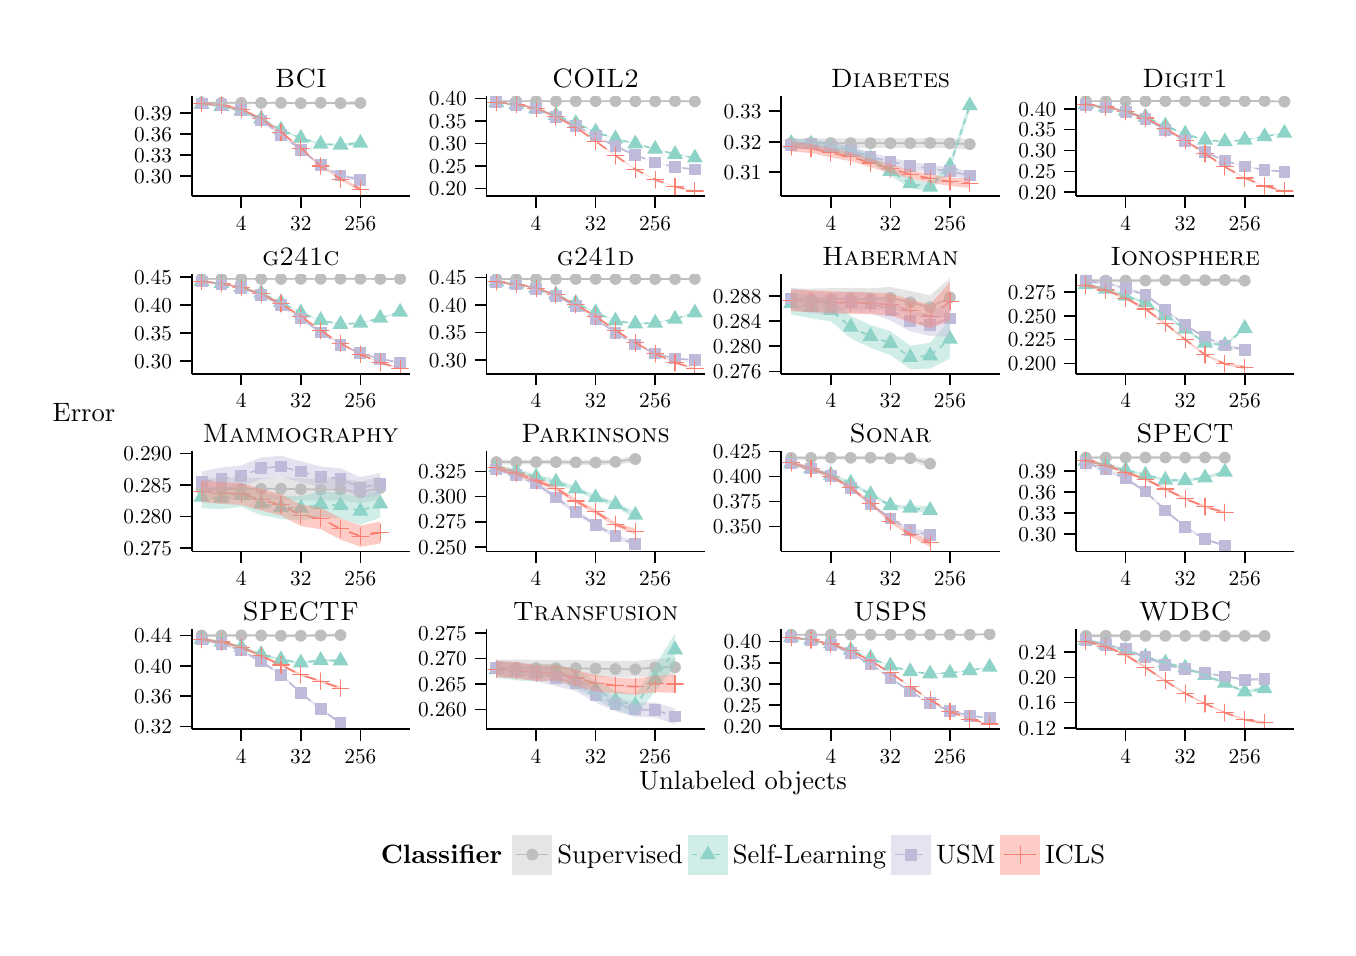
\begin{tikzpicture}[x=1pt,y=1pt]
\definecolor{fillColor}{RGB}{255,255,255}
\path[use as bounding box,fill=fillColor,fill opacity=0.00] (0,0) rectangle (469.75,325.21);
\begin{scope}
\path[clip] (  0.00,  0.00) rectangle (469.75,325.21);
\definecolor{drawColor}{RGB}{255,255,255}
\definecolor{fillColor}{RGB}{255,255,255}

\path[draw=drawColor,line width= 0.6pt,line join=round,line cap=round,fill=fillColor] (  0.00,  0.00) rectangle (469.76,325.21);
\end{scope}
\begin{scope}
\path[clip] ( 59.26,264.38) rectangle (138.16,300.54);
\definecolor{fillColor}{RGB}{255,255,255}

\path[fill=fillColor] ( 59.26,264.38) rectangle (138.16,300.54);
\definecolor{fillColor}{RGB}{190,190,190}

\path[fill=fillColor] ( 62.84,298.08) circle (  2.13);
\definecolor{fillColor}{RGB}{141,211,199}

\path[fill=fillColor] ( 62.84,300.94) --
	( 65.72,295.97) --
	( 59.97,295.97) --
	cycle;
\definecolor{fillColor}{RGB}{190,186,218}

\path[fill=fillColor] ( 60.71,295.66) --
	( 64.98,295.66) --
	( 64.98,299.92) --
	( 60.71,299.92) --
	cycle;
\definecolor{drawColor}{RGB}{251,128,114}

\path[draw=drawColor,line width= 0.4pt,line join=round,line cap=round] ( 59.82,297.81) -- ( 65.86,297.81);

\path[draw=drawColor,line width= 0.4pt,line join=round,line cap=round] ( 62.84,294.79) -- ( 62.84,300.82);
\definecolor{fillColor}{RGB}{190,190,190}

\path[fill=fillColor] ( 70.01,298.07) circle (  2.13);
\definecolor{fillColor}{RGB}{141,211,199}

\path[fill=fillColor] ( 70.01,300.11) --
	( 72.89,295.13) --
	( 67.14,295.13) --
	cycle;
\definecolor{fillColor}{RGB}{190,186,218}

\path[fill=fillColor] ( 67.88,295.03) --
	( 72.15,295.03) --
	( 72.15,299.30) --
	( 67.88,299.30) --
	cycle;

\path[draw=drawColor,line width= 0.4pt,line join=round,line cap=round] ( 67.00,297.24) -- ( 73.03,297.24);

\path[draw=drawColor,line width= 0.4pt,line join=round,line cap=round] ( 70.01,294.22) -- ( 70.01,300.26);
\definecolor{fillColor}{RGB}{190,190,190}

\path[fill=fillColor] ( 77.19,298.03) circle (  2.13);
\definecolor{fillColor}{RGB}{141,211,199}

\path[fill=fillColor] ( 77.19,298.45) --
	( 80.06,293.47) --
	( 74.31,293.47) --
	cycle;
\definecolor{fillColor}{RGB}{190,186,218}

\path[fill=fillColor] ( 75.05,293.19) --
	( 79.32,293.19) --
	( 79.32,297.46) --
	( 75.05,297.46) --
	cycle;

\path[draw=drawColor,line width= 0.4pt,line join=round,line cap=round] ( 74.17,295.65) -- ( 80.21,295.65);

\path[draw=drawColor,line width= 0.4pt,line join=round,line cap=round] ( 77.19,292.63) -- ( 77.19,298.67);
\definecolor{fillColor}{RGB}{190,190,190}

\path[fill=fillColor] ( 84.36,298.01) circle (  2.13);
\definecolor{fillColor}{RGB}{141,211,199}

\path[fill=fillColor] ( 84.36,295.64) --
	( 87.23,290.66) --
	( 81.49,290.66) --
	cycle;
\definecolor{fillColor}{RGB}{190,186,218}

\path[fill=fillColor] ( 82.23,289.56) --
	( 86.49,289.56) --
	( 86.49,293.83) --
	( 82.23,293.83) --
	cycle;

\path[draw=drawColor,line width= 0.4pt,line join=round,line cap=round] ( 81.34,292.39) -- ( 87.38,292.39);

\path[draw=drawColor,line width= 0.4pt,line join=round,line cap=round] ( 84.36,289.37) -- ( 84.36,295.41);
\definecolor{fillColor}{RGB}{190,190,190}

\path[fill=fillColor] ( 91.53,298.03) circle (  2.13);
\definecolor{fillColor}{RGB}{141,211,199}

\path[fill=fillColor] ( 91.53,291.62) --
	( 94.41,286.64) --
	( 88.66,286.64) --
	cycle;
\definecolor{fillColor}{RGB}{190,186,218}

\path[fill=fillColor] ( 89.40,284.41) --
	( 93.67,284.41) --
	( 93.67,288.68) --
	( 89.40,288.68) --
	cycle;

\path[draw=drawColor,line width= 0.4pt,line join=round,line cap=round] ( 88.52,287.41) -- ( 94.55,287.41);

\path[draw=drawColor,line width= 0.4pt,line join=round,line cap=round] ( 91.53,284.40) -- ( 91.53,290.43);
\definecolor{fillColor}{RGB}{190,190,190}

\path[fill=fillColor] ( 98.71,297.91) circle (  2.13);
\definecolor{fillColor}{RGB}{141,211,199}

\path[fill=fillColor] ( 98.71,288.61) --
	(101.58,283.63) --
	( 95.83,283.63) --
	cycle;
\definecolor{fillColor}{RGB}{190,186,218}

\path[fill=fillColor] ( 96.57,278.91) --
	(100.84,278.91) --
	(100.84,283.18) --
	( 96.57,283.18) --
	cycle;

\path[draw=drawColor,line width= 0.4pt,line join=round,line cap=round] ( 95.69,281.69) -- (101.72,281.69);

\path[draw=drawColor,line width= 0.4pt,line join=round,line cap=round] ( 98.71,278.68) -- ( 98.71,284.71);
\definecolor{fillColor}{RGB}{190,190,190}

\path[fill=fillColor] (105.88,298.06) circle (  2.13);
\definecolor{fillColor}{RGB}{141,211,199}

\path[fill=fillColor] (105.88,286.47) --
	(108.75,281.49) --
	(103.01,281.49) --
	cycle;
\definecolor{fillColor}{RGB}{190,186,218}

\path[fill=fillColor] (103.75,273.32) --
	(108.01,273.32) --
	(108.01,277.59) --
	(103.75,277.59) --
	cycle;

\path[draw=drawColor,line width= 0.4pt,line join=round,line cap=round] (102.86,275.23) -- (108.90,275.23);

\path[draw=drawColor,line width= 0.4pt,line join=round,line cap=round] (105.88,272.21) -- (105.88,278.25);
\definecolor{fillColor}{RGB}{190,190,190}

\path[fill=fillColor] (113.05,297.92) circle (  2.13);
\definecolor{fillColor}{RGB}{141,211,199}

\path[fill=fillColor] (113.05,286.16) --
	(115.93,281.18) --
	(110.18,281.18) --
	cycle;
\definecolor{fillColor}{RGB}{190,186,218}

\path[fill=fillColor] (110.92,269.68) --
	(115.19,269.68) --
	(115.19,273.95) --
	(110.92,273.95) --
	cycle;

\path[draw=drawColor,line width= 0.4pt,line join=round,line cap=round] (110.04,270.49) -- (116.07,270.49);

\path[draw=drawColor,line width= 0.4pt,line join=round,line cap=round] (113.05,267.48) -- (113.05,273.51);
\definecolor{fillColor}{RGB}{190,190,190}

\path[fill=fillColor] (120.23,298.00) circle (  2.13);
\definecolor{fillColor}{RGB}{141,211,199}

\path[fill=fillColor] (120.23,286.82) --
	(123.10,281.84) --
	(117.35,281.84) --
	cycle;
\definecolor{fillColor}{RGB}{190,186,218}

\path[fill=fillColor] (118.09,268.11) --
	(122.36,268.11) --
	(122.36,272.38) --
	(118.09,272.38) --
	cycle;

\path[draw=drawColor,line width= 0.4pt,line join=round,line cap=round] (117.21,266.81) -- (123.24,266.81);

\path[draw=drawColor,line width= 0.4pt,line join=round,line cap=round] (120.23,263.80) -- (120.23,269.83);
\definecolor{drawColor}{RGB}{190,190,190}

\path[draw=drawColor,line width= 0.6pt,line join=round] ( 62.84,298.08) --
	( 70.01,298.07) --
	( 77.19,298.03) --
	( 84.36,298.01) --
	( 91.53,298.03) --
	( 98.71,297.91) --
	(105.88,298.06) --
	(113.05,297.92) --
	(120.23,298.00);
\definecolor{drawColor}{RGB}{141,211,199}

\path[draw=drawColor,line width= 0.6pt,dash pattern=on 2pt off 2pt ,line join=round] ( 62.84,297.63) --
	( 70.01,296.79) --
	( 77.19,295.13) --
	( 84.36,292.32) --
	( 91.53,288.30) --
	( 98.71,285.29) --
	(105.88,283.15) --
	(113.05,282.84) --
	(120.23,283.50);
\definecolor{drawColor}{RGB}{190,186,218}

\path[draw=drawColor,line width= 0.6pt,dash pattern=on 4pt off 2pt ,line join=round] ( 62.84,297.79) --
	( 70.01,297.17) --
	( 77.19,295.33) --
	( 84.36,291.70) --
	( 91.53,286.55) --
	( 98.71,281.05) --
	(105.88,275.45) --
	(113.05,271.81) --
	(120.23,270.25);
\definecolor{drawColor}{RGB}{251,128,114}

\path[draw=drawColor,line width= 0.6pt,dash pattern=on 4pt off 4pt ,line join=round] ( 62.84,297.81) --
	( 70.01,297.24) --
	( 77.19,295.65) --
	( 84.36,292.39) --
	( 91.53,287.41) --
	( 98.71,281.69) --
	(105.88,275.23) --
	(113.05,270.49) --
	(120.23,266.81);
\definecolor{fillColor}{RGB}{190,190,190}

\path[fill=fillColor,fill opacity=0.40] ( 62.84,298.44) --
	( 70.01,298.43) --
	( 77.19,298.39) --
	( 84.36,298.37) --
	( 91.53,298.40) --
	( 98.71,298.28) --
	(105.88,298.45) --
	(113.05,298.35) --
	(120.23,298.89) --
	(120.23,297.10) --
	(113.05,297.48) --
	(105.88,297.67) --
	( 98.71,297.54) --
	( 91.53,297.66) --
	( 84.36,297.64) --
	( 77.19,297.67) --
	( 70.01,297.71) --
	( 62.84,297.72) --
	cycle;
\definecolor{fillColor}{RGB}{141,211,199}

\path[fill=fillColor,fill opacity=0.40] ( 62.84,297.99) --
	( 70.01,297.15) --
	( 77.19,295.47) --
	( 84.36,292.66) --
	( 91.53,288.65) --
	( 98.71,285.62) --
	(105.88,283.49) --
	(113.05,283.22) --
	(120.23,284.33) --
	(120.23,282.67) --
	(113.05,282.46) --
	(105.88,282.81) --
	( 98.71,284.97) --
	( 91.53,287.96) --
	( 84.36,291.98) --
	( 77.19,294.79) --
	( 70.01,296.43) --
	( 62.84,297.27) --
	cycle;
\definecolor{fillColor}{RGB}{190,186,218}

\path[fill=fillColor,fill opacity=0.40] ( 62.84,298.15) --
	( 70.01,297.53) --
	( 77.19,295.68) --
	( 84.36,292.04) --
	( 91.53,286.90) --
	( 98.71,281.37) --
	(105.88,275.77) --
	(113.05,272.15) --
	(120.23,271.05) --
	(120.23,269.44) --
	(113.05,271.47) --
	(105.88,275.14) --
	( 98.71,280.73) --
	( 91.53,286.20) --
	( 84.36,291.35) --
	( 77.19,294.97) --
	( 70.01,296.80) --
	( 62.84,297.43) --
	cycle;
\definecolor{fillColor}{RGB}{251,128,114}

\path[fill=fillColor,fill opacity=0.40] ( 62.84,298.17) --
	( 70.01,297.60) --
	( 77.19,296.01) --
	( 84.36,292.73) --
	( 91.53,287.76) --
	( 98.71,282.02) --
	(105.88,275.55) --
	(113.05,270.84) --
	(120.23,267.60) --
	(120.23,266.03) --
	(113.05,270.15) --
	(105.88,274.91) --
	( 98.71,281.37) --
	( 91.53,287.07) --
	( 84.36,292.05) --
	( 77.19,295.30) --
	( 70.01,296.88) --
	( 62.84,297.44) --
	cycle;
\end{scope}
\begin{scope}
\path[clip] (165.77,264.38) rectangle (244.68,300.54);
\definecolor{fillColor}{RGB}{255,255,255}

\path[fill=fillColor] (165.77,264.38) rectangle (244.68,300.54);
\definecolor{fillColor}{RGB}{190,190,190}

\path[fill=fillColor] (169.36,298.66) circle (  2.13);
\definecolor{fillColor}{RGB}{141,211,199}

\path[fill=fillColor] (169.36,301.50) --
	(172.23,296.52) --
	(166.48,296.52) --
	cycle;
\definecolor{fillColor}{RGB}{190,186,218}

\path[fill=fillColor] (167.22,296.15) --
	(171.49,296.15) --
	(171.49,300.41) --
	(167.22,300.41) --
	cycle;
\definecolor{drawColor}{RGB}{251,128,114}

\path[draw=drawColor,line width= 0.4pt,line join=round,line cap=round] (166.34,298.26) -- (172.38,298.26);

\path[draw=drawColor,line width= 0.4pt,line join=round,line cap=round] (169.36,295.24) -- (169.36,301.28);
\definecolor{fillColor}{RGB}{190,190,190}

\path[fill=fillColor] (176.53,298.66) circle (  2.13);
\definecolor{fillColor}{RGB}{141,211,199}

\path[fill=fillColor] (176.53,300.75) --
	(179.41,295.78) --
	(173.66,295.78) --
	cycle;
\definecolor{fillColor}{RGB}{190,186,218}

\path[fill=fillColor] (174.40,295.25) --
	(178.67,295.25) --
	(178.67,299.52) --
	(174.40,299.52) --
	cycle;

\path[draw=drawColor,line width= 0.4pt,line join=round,line cap=round] (173.51,297.53) -- (179.55,297.53);

\path[draw=drawColor,line width= 0.4pt,line join=round,line cap=round] (176.53,294.51) -- (176.53,300.55);
\definecolor{fillColor}{RGB}{190,190,190}

\path[fill=fillColor] (183.71,298.66) circle (  2.13);
\definecolor{fillColor}{RGB}{141,211,199}

\path[fill=fillColor] (183.71,299.39) --
	(186.58,294.41) --
	(180.83,294.41) --
	cycle;
\definecolor{fillColor}{RGB}{190,186,218}

\path[fill=fillColor] (181.57,293.85) --
	(185.84,293.85) --
	(185.84,298.12) --
	(181.57,298.12) --
	cycle;

\path[draw=drawColor,line width= 0.4pt,line join=round,line cap=round] (180.69,296.09) -- (186.72,296.09);

\path[draw=drawColor,line width= 0.4pt,line join=round,line cap=round] (183.71,293.08) -- (183.71,299.11);
\definecolor{fillColor}{RGB}{190,190,190}

\path[fill=fillColor] (190.88,298.66) circle (  2.13);
\definecolor{fillColor}{RGB}{141,211,199}

\path[fill=fillColor] (190.88,296.91) --
	(193.75,291.93) --
	(188.00,291.93) --
	cycle;
\definecolor{fillColor}{RGB}{190,186,218}

\path[fill=fillColor] (188.74,290.94) --
	(193.01,290.94) --
	(193.01,295.21) --
	(188.74,295.21) --
	cycle;

\path[draw=drawColor,line width= 0.4pt,line join=round,line cap=round] (187.86,293.08) -- (193.90,293.08);

\path[draw=drawColor,line width= 0.4pt,line join=round,line cap=round] (190.88,290.06) -- (190.88,296.10);
\definecolor{fillColor}{RGB}{190,190,190}

\path[fill=fillColor] (198.05,298.66) circle (  2.13);
\definecolor{fillColor}{RGB}{141,211,199}

\path[fill=fillColor] (198.05,293.99) --
	(200.93,289.02) --
	(195.18,289.02) --
	cycle;
\definecolor{fillColor}{RGB}{190,186,218}

\path[fill=fillColor] (195.92,287.66) --
	(200.19,287.66) --
	(200.19,291.93) --
	(195.92,291.93) --
	cycle;

\path[draw=drawColor,line width= 0.4pt,line join=round,line cap=round] (195.03,289.20) -- (201.07,289.20);

\path[draw=drawColor,line width= 0.4pt,line join=round,line cap=round] (198.05,286.19) -- (198.05,292.22);
\definecolor{fillColor}{RGB}{190,190,190}

\path[fill=fillColor] (205.22,298.67) circle (  2.13);
\definecolor{fillColor}{RGB}{141,211,199}

\path[fill=fillColor] (205.22,290.89) --
	(208.10,285.91) --
	(202.35,285.91) --
	cycle;
\definecolor{fillColor}{RGB}{190,186,218}

\path[fill=fillColor] (203.09,283.84) --
	(207.36,283.84) --
	(207.36,288.11) --
	(203.09,288.11) --
	cycle;

\path[draw=drawColor,line width= 0.4pt,line join=round,line cap=round] (202.21,284.20) -- (208.24,284.20);

\path[draw=drawColor,line width= 0.4pt,line join=round,line cap=round] (205.22,281.18) -- (205.22,287.22);
\definecolor{fillColor}{RGB}{190,190,190}

\path[fill=fillColor] (212.40,298.66) circle (  2.13);
\definecolor{fillColor}{RGB}{141,211,199}

\path[fill=fillColor] (212.40,288.40) --
	(215.27,283.42) --
	(209.52,283.42) --
	cycle;
\definecolor{fillColor}{RGB}{190,186,218}

\path[fill=fillColor] (210.26,280.18) --
	(214.53,280.18) --
	(214.53,284.44) --
	(210.26,284.44) --
	cycle;

\path[draw=drawColor,line width= 0.4pt,line join=round,line cap=round] (209.38,278.96) -- (215.42,278.96);

\path[draw=drawColor,line width= 0.4pt,line join=round,line cap=round] (212.40,275.94) -- (212.40,281.98);
\definecolor{fillColor}{RGB}{190,190,190}

\path[fill=fillColor] (219.57,298.65) circle (  2.13);
\definecolor{fillColor}{RGB}{141,211,199}

\path[fill=fillColor] (219.57,286.58) --
	(222.44,281.60) --
	(216.70,281.60) --
	cycle;
\definecolor{fillColor}{RGB}{190,186,218}

\path[fill=fillColor] (217.44,277.00) --
	(221.70,277.00) --
	(221.70,281.27) --
	(217.44,281.27) --
	cycle;

\path[draw=drawColor,line width= 0.4pt,line join=round,line cap=round] (216.55,274.05) -- (222.59,274.05);

\path[draw=drawColor,line width= 0.4pt,line join=round,line cap=round] (219.57,271.03) -- (219.57,277.07);
\definecolor{fillColor}{RGB}{190,190,190}

\path[fill=fillColor] (226.74,298.65) circle (  2.13);
\definecolor{fillColor}{RGB}{141,211,199}

\path[fill=fillColor] (226.74,284.67) --
	(229.62,279.69) --
	(223.87,279.69) --
	cycle;
\definecolor{fillColor}{RGB}{190,186,218}

\path[fill=fillColor] (224.61,274.37) --
	(228.88,274.37) --
	(228.88,278.64) --
	(224.61,278.64) --
	cycle;

\path[draw=drawColor,line width= 0.4pt,line join=round,line cap=round] (223.73,270.27) -- (229.76,270.27);

\path[draw=drawColor,line width= 0.4pt,line join=round,line cap=round] (226.74,267.25) -- (226.74,273.29);
\definecolor{fillColor}{RGB}{190,190,190}

\path[fill=fillColor] (233.92,298.69) circle (  2.13);
\definecolor{fillColor}{RGB}{141,211,199}

\path[fill=fillColor] (233.92,282.78) --
	(236.79,277.80) --
	(231.04,277.80) --
	cycle;
\definecolor{fillColor}{RGB}{190,186,218}

\path[fill=fillColor] (231.78,272.71) --
	(236.05,272.71) --
	(236.05,276.98) --
	(231.78,276.98) --
	cycle;

\path[draw=drawColor,line width= 0.4pt,line join=round,line cap=round] (230.90,267.75) -- (236.93,267.75);

\path[draw=drawColor,line width= 0.4pt,line join=round,line cap=round] (233.92,264.73) -- (233.92,270.76);
\definecolor{fillColor}{RGB}{190,190,190}

\path[fill=fillColor] (241.09,298.56) circle (  2.13);
\definecolor{fillColor}{RGB}{141,211,199}

\path[fill=fillColor] (241.09,281.47) --
	(243.96,276.50) --
	(238.22,276.50) --
	cycle;
\definecolor{fillColor}{RGB}{190,186,218}

\path[fill=fillColor] (238.96,271.84) --
	(243.22,271.84) --
	(243.22,276.11) --
	(238.96,276.11) --
	cycle;

\path[draw=drawColor,line width= 0.4pt,line join=round,line cap=round] (238.07,266.17) -- (244.11,266.17);

\path[draw=drawColor,line width= 0.4pt,line join=round,line cap=round] (241.09,263.15) -- (241.09,269.19);
\definecolor{drawColor}{RGB}{190,190,190}

\path[draw=drawColor,line width= 0.6pt,line join=round] (169.36,298.66) --
	(176.53,298.66) --
	(183.71,298.66) --
	(190.88,298.66) --
	(198.05,298.66) --
	(205.22,298.67) --
	(212.40,298.66) --
	(219.57,298.65) --
	(226.74,298.65) --
	(233.92,298.69) --
	(241.09,298.56);
\definecolor{drawColor}{RGB}{141,211,199}

\path[draw=drawColor,line width= 0.6pt,dash pattern=on 2pt off 2pt ,line join=round] (169.36,298.18) --
	(176.53,297.43) --
	(183.71,296.07) --
	(190.88,293.59) --
	(198.05,290.68) --
	(205.22,287.57) --
	(212.40,285.08) --
	(219.57,283.26) --
	(226.74,281.35) --
	(233.92,279.46) --
	(241.09,278.16);
\definecolor{drawColor}{RGB}{190,186,218}

\path[draw=drawColor,line width= 0.6pt,dash pattern=on 4pt off 2pt ,line join=round] (169.36,298.28) --
	(176.53,297.38) --
	(183.71,295.99) --
	(190.88,293.08) --
	(198.05,289.79) --
	(205.22,285.98) --
	(212.40,282.31) --
	(219.57,279.14) --
	(226.74,276.51) --
	(233.92,274.85) --
	(241.09,273.98);
\definecolor{drawColor}{RGB}{251,128,114}

\path[draw=drawColor,line width= 0.6pt,dash pattern=on 4pt off 4pt ,line join=round] (169.36,298.26) --
	(176.53,297.53) --
	(183.71,296.09) --
	(190.88,293.08) --
	(198.05,289.20) --
	(205.22,284.20) --
	(212.40,278.96) --
	(219.57,274.05) --
	(226.74,270.27) --
	(233.92,267.75) --
	(241.09,266.17);
\definecolor{fillColor}{RGB}{190,190,190}

\path[fill=fillColor,fill opacity=0.40] (169.36,298.85) --
	(176.53,298.85) --
	(183.71,298.85) --
	(190.88,298.85) --
	(198.05,298.85) --
	(205.22,298.86) --
	(212.40,298.85) --
	(219.57,298.84) --
	(226.74,298.84) --
	(233.92,298.89) --
	(241.09,298.80) --
	(241.09,298.31) --
	(233.92,298.50) --
	(226.74,298.45) --
	(219.57,298.46) --
	(212.40,298.47) --
	(205.22,298.48) --
	(198.05,298.47) --
	(190.88,298.46) --
	(183.71,298.47) --
	(176.53,298.47) --
	(169.36,298.47) --
	cycle;
\definecolor{fillColor}{RGB}{141,211,199}

\path[fill=fillColor,fill opacity=0.40] (169.36,298.38) --
	(176.53,297.63) --
	(183.71,296.26) --
	(190.88,293.77) --
	(198.05,290.85) --
	(205.22,287.73) --
	(212.40,285.23) --
	(219.57,283.41) --
	(226.74,281.49) --
	(233.92,279.62) --
	(241.09,278.36) --
	(241.09,277.95) --
	(233.92,279.30) --
	(226.74,281.20) --
	(219.57,283.12) --
	(212.40,284.94) --
	(205.22,287.41) --
	(198.05,290.50) --
	(190.88,293.41) --
	(183.71,295.89) --
	(176.53,297.24) --
	(169.36,297.99) --
	cycle;
\definecolor{fillColor}{RGB}{190,186,218}

\path[fill=fillColor,fill opacity=0.40] (169.36,298.47) --
	(176.53,297.58) --
	(183.71,296.17) --
	(190.88,293.26) --
	(198.05,289.96) --
	(205.22,286.12) --
	(212.40,282.44) --
	(219.57,279.26) --
	(226.74,276.61) --
	(233.92,274.95) --
	(241.09,274.13) --
	(241.09,273.83) --
	(233.92,274.74) --
	(226.74,276.40) --
	(219.57,279.02) --
	(212.40,282.18) --
	(205.22,285.83) --
	(198.05,289.62) --
	(190.88,292.90) --
	(183.71,295.80) --
	(176.53,297.19) --
	(169.36,298.09) --
	cycle;
\definecolor{fillColor}{RGB}{251,128,114}

\path[fill=fillColor,fill opacity=0.40] (169.36,298.45) --
	(176.53,297.72) --
	(183.71,296.28) --
	(190.88,293.26) --
	(198.05,289.38) --
	(205.22,284.36) --
	(212.40,279.10) --
	(219.57,274.17) --
	(226.74,270.37) --
	(233.92,267.85) --
	(241.09,266.32) --
	(241.09,266.03) --
	(233.92,267.64) --
	(226.74,270.16) --
	(219.57,273.93) --
	(212.40,278.82) --
	(205.22,284.04) --
	(198.05,289.03) --
	(190.88,292.90) --
	(183.71,295.91) --
	(176.53,297.34) --
	(169.36,298.07) --
	cycle;
\end{scope}
\begin{scope}
\path[clip] (272.29,264.38) rectangle (351.19,300.54);
\definecolor{fillColor}{RGB}{255,255,255}

\path[fill=fillColor] (272.29,264.38) rectangle (351.19,300.54);
\definecolor{fillColor}{RGB}{190,190,190}

\path[fill=fillColor] (275.88,283.52) circle (  2.13);
\definecolor{fillColor}{RGB}{141,211,199}

\path[fill=fillColor] (275.88,286.71) --
	(278.75,281.74) --
	(273.00,281.74) --
	cycle;
\definecolor{fillColor}{RGB}{190,186,218}

\path[fill=fillColor] (273.74,280.76) --
	(278.01,280.76) --
	(278.01,285.03) --
	(273.74,285.03) --
	cycle;
\definecolor{drawColor}{RGB}{251,128,114}

\path[draw=drawColor,line width= 0.4pt,line join=round,line cap=round] (272.86,282.19) -- (278.89,282.19);

\path[draw=drawColor,line width= 0.4pt,line join=round,line cap=round] (275.88,279.17) -- (275.88,285.21);
\definecolor{fillColor}{RGB}{190,190,190}

\path[fill=fillColor] (283.05,283.50) circle (  2.13);
\definecolor{fillColor}{RGB}{141,211,199}

\path[fill=fillColor] (283.05,286.51) --
	(285.92,281.53) --
	(280.18,281.53) --
	cycle;
\definecolor{fillColor}{RGB}{190,186,218}

\path[fill=fillColor] (280.92,281.20) --
	(285.18,281.20) --
	(285.18,285.47) --
	(280.92,285.47) --
	cycle;

\path[draw=drawColor,line width= 0.4pt,line join=round,line cap=round] (280.03,281.57) -- (286.07,281.57);

\path[draw=drawColor,line width= 0.4pt,line join=round,line cap=round] (283.05,278.55) -- (283.05,284.58);
\definecolor{fillColor}{RGB}{190,190,190}

\path[fill=fillColor] (290.22,283.51) circle (  2.13);
\definecolor{fillColor}{RGB}{141,211,199}

\path[fill=fillColor] (290.22,285.22) --
	(293.10,280.24) --
	(287.35,280.24) --
	cycle;
\definecolor{fillColor}{RGB}{190,186,218}

\path[fill=fillColor] (288.09,279.88) --
	(292.36,279.88) --
	(292.36,284.15) --
	(288.09,284.15) --
	cycle;

\path[draw=drawColor,line width= 0.4pt,line join=round,line cap=round] (287.20,279.97) -- (293.24,279.97);

\path[draw=drawColor,line width= 0.4pt,line join=round,line cap=round] (290.22,276.95) -- (290.22,282.99);
\definecolor{fillColor}{RGB}{190,190,190}

\path[fill=fillColor] (297.40,283.49) circle (  2.13);
\definecolor{fillColor}{RGB}{141,211,199}

\path[fill=fillColor] (297.40,283.82) --
	(300.27,278.84) --
	(294.52,278.84) --
	cycle;
\definecolor{fillColor}{RGB}{190,186,218}

\path[fill=fillColor] (295.26,278.81) --
	(299.53,278.81) --
	(299.53,283.08) --
	(295.26,283.08) --
	cycle;

\path[draw=drawColor,line width= 0.4pt,line join=round,line cap=round] (294.38,278.59) -- (300.41,278.59);

\path[draw=drawColor,line width= 0.4pt,line join=round,line cap=round] (297.40,275.57) -- (297.40,281.61);
\definecolor{fillColor}{RGB}{190,190,190}

\path[fill=fillColor] (304.57,283.47) circle (  2.13);
\definecolor{fillColor}{RGB}{141,211,199}

\path[fill=fillColor] (304.57,281.30) --
	(307.44,276.32) --
	(301.69,276.32) --
	cycle;
\definecolor{fillColor}{RGB}{190,186,218}

\path[fill=fillColor] (302.43,276.43) --
	(306.70,276.43) --
	(306.70,280.70) --
	(302.43,280.70) --
	cycle;

\path[draw=drawColor,line width= 0.4pt,line join=round,line cap=round] (301.55,276.31) -- (307.59,276.31);

\path[draw=drawColor,line width= 0.4pt,line join=round,line cap=round] (304.57,273.29) -- (304.57,279.33);
\definecolor{fillColor}{RGB}{190,190,190}

\path[fill=fillColor] (311.74,283.48) circle (  2.13);
\definecolor{fillColor}{RGB}{141,211,199}

\path[fill=fillColor] (311.74,276.67) --
	(314.62,271.69) --
	(308.87,271.69) --
	cycle;
\definecolor{fillColor}{RGB}{190,186,218}

\path[fill=fillColor] (309.61,274.71) --
	(313.88,274.71) --
	(313.88,278.98) --
	(309.61,278.98) --
	cycle;

\path[draw=drawColor,line width= 0.4pt,line join=round,line cap=round] (308.72,274.26) -- (314.76,274.26);

\path[draw=drawColor,line width= 0.4pt,line join=round,line cap=round] (311.74,271.24) -- (311.74,277.28);
\definecolor{fillColor}{RGB}{190,190,190}

\path[fill=fillColor] (318.91,283.46) circle (  2.13);
\definecolor{fillColor}{RGB}{141,211,199}

\path[fill=fillColor] (318.91,272.18) --
	(321.79,267.20) --
	(316.04,267.20) --
	cycle;
\definecolor{fillColor}{RGB}{190,186,218}

\path[fill=fillColor] (316.78,273.15) --
	(321.05,273.15) --
	(321.05,277.41) --
	(316.78,277.41) --
	cycle;

\path[draw=drawColor,line width= 0.4pt,line join=round,line cap=round] (315.90,272.23) -- (321.93,272.23);

\path[draw=drawColor,line width= 0.4pt,line join=round,line cap=round] (318.91,269.22) -- (318.91,275.25);
\definecolor{fillColor}{RGB}{190,190,190}

\path[fill=fillColor] (326.09,283.54) circle (  2.13);
\definecolor{fillColor}{RGB}{141,211,199}

\path[fill=fillColor] (326.09,270.93) --
	(328.96,265.96) --
	(323.21,265.96) --
	cycle;
\definecolor{fillColor}{RGB}{190,186,218}

\path[fill=fillColor] (323.95,272.14) --
	(328.22,272.14) --
	(328.22,276.41) --
	(323.95,276.41) --
	cycle;

\path[draw=drawColor,line width= 0.4pt,line join=round,line cap=round] (323.07,270.72) -- (329.11,270.72);

\path[draw=drawColor,line width= 0.4pt,line join=round,line cap=round] (326.09,267.71) -- (326.09,273.74);
\definecolor{fillColor}{RGB}{190,190,190}

\path[fill=fillColor] (333.26,283.42) circle (  2.13);
\definecolor{fillColor}{RGB}{141,211,199}

\path[fill=fillColor] (333.26,278.58) --
	(336.13,273.60) --
	(330.39,273.60) --
	cycle;
\definecolor{fillColor}{RGB}{190,186,218}

\path[fill=fillColor] (331.13,271.16) --
	(335.39,271.16) --
	(335.39,275.42) --
	(331.13,275.42) --
	cycle;

\path[draw=drawColor,line width= 0.4pt,line join=round,line cap=round] (330.24,269.57) -- (336.28,269.57);

\path[draw=drawColor,line width= 0.4pt,line join=round,line cap=round] (333.26,266.55) -- (333.26,272.58);
\definecolor{fillColor}{RGB}{190,190,190}

\path[fill=fillColor] (340.43,283.11) circle (  2.13);
\definecolor{fillColor}{RGB}{141,211,199}

\path[fill=fillColor] (340.43,300.39) --
	(343.31,295.41) --
	(337.56,295.41) --
	cycle;
\definecolor{fillColor}{RGB}{190,186,218}

\path[fill=fillColor] (338.30,269.67) --
	(342.57,269.67) --
	(342.57,273.94) --
	(338.30,273.94) --
	cycle;

\path[draw=drawColor,line width= 0.4pt,line join=round,line cap=round] (337.42,268.98) -- (343.45,268.98);

\path[draw=drawColor,line width= 0.4pt,line join=round,line cap=round] (340.43,265.96) -- (340.43,272.00);
\definecolor{drawColor}{RGB}{190,190,190}

\path[draw=drawColor,line width= 0.6pt,line join=round] (275.88,283.52) --
	(283.05,283.50) --
	(290.22,283.51) --
	(297.40,283.49) --
	(304.57,283.47) --
	(311.74,283.48) --
	(318.91,283.46) --
	(326.09,283.54) --
	(333.26,283.42) --
	(340.43,283.11);
\definecolor{drawColor}{RGB}{141,211,199}

\path[draw=drawColor,line width= 0.6pt,dash pattern=on 2pt off 2pt ,line join=round] (275.88,283.39) --
	(283.05,283.19) --
	(290.22,281.90) --
	(297.40,280.50) --
	(304.57,277.98) --
	(311.74,273.35) --
	(318.91,268.86) --
	(326.09,267.62) --
	(333.26,275.26) --
	(340.43,297.07);
\definecolor{drawColor}{RGB}{190,186,218}

\path[draw=drawColor,line width= 0.6pt,dash pattern=on 4pt off 2pt ,line join=round] (275.88,282.89) --
	(283.05,283.34) --
	(290.22,282.02) --
	(297.40,280.95) --
	(304.57,278.56) --
	(311.74,276.84) --
	(318.91,275.28) --
	(326.09,274.28) --
	(333.26,273.29) --
	(340.43,271.80);
\definecolor{drawColor}{RGB}{251,128,114}

\path[draw=drawColor,line width= 0.6pt,dash pattern=on 4pt off 4pt ,line join=round] (275.88,282.19) --
	(283.05,281.57) --
	(290.22,279.97) --
	(297.40,278.59) --
	(304.57,276.31) --
	(311.74,274.26) --
	(318.91,272.23) --
	(326.09,270.72) --
	(333.26,269.57) --
	(340.43,268.98);
\definecolor{fillColor}{RGB}{190,190,190}

\path[fill=fillColor,fill opacity=0.40] (275.88,285.24) --
	(283.05,285.22) --
	(290.22,285.23) --
	(297.40,285.21) --
	(304.57,285.19) --
	(311.74,285.21) --
	(318.91,285.19) --
	(326.09,285.28) --
	(333.26,285.19) --
	(340.43,285.00) --
	(340.43,281.22) --
	(333.26,281.65) --
	(326.09,281.80) --
	(318.91,281.74) --
	(311.74,281.76) --
	(304.57,281.76) --
	(297.40,281.77) --
	(290.22,281.80) --
	(283.05,281.79) --
	(275.88,281.81) --
	cycle;
\definecolor{fillColor}{RGB}{141,211,199}

\path[fill=fillColor,fill opacity=0.40] (275.88,285.09) --
	(283.05,284.87) --
	(290.22,283.59) --
	(297.40,282.16) --
	(304.57,279.62) --
	(311.74,274.98) --
	(318.91,270.51) --
	(326.09,269.20) --
	(333.26,276.95) --
	(340.43,298.89) --
	(340.43,295.25) --
	(333.26,273.57) --
	(326.09,266.03) --
	(318.91,267.20) --
	(311.74,271.71) --
	(304.57,276.34) --
	(297.40,278.83) --
	(290.22,280.21) --
	(283.05,281.51) --
	(275.88,281.70) --
	cycle;
\definecolor{fillColor}{RGB}{190,186,218}

\path[fill=fillColor,fill opacity=0.40] (275.88,284.55) --
	(283.05,284.98) --
	(290.22,283.64) --
	(297.40,282.47) --
	(304.57,280.03) --
	(311.74,278.28) --
	(318.91,276.71) --
	(326.09,275.70) --
	(333.26,274.73) --
	(340.43,273.41) --
	(340.43,270.20) --
	(333.26,271.85) --
	(326.09,272.85) --
	(318.91,273.85) --
	(311.74,275.41) --
	(304.57,277.10) --
	(297.40,279.42) --
	(290.22,280.40) --
	(283.05,281.69) --
	(275.88,281.23) --
	cycle;
\definecolor{fillColor}{RGB}{251,128,114}

\path[fill=fillColor,fill opacity=0.40] (275.88,283.87) --
	(283.05,283.23) --
	(290.22,281.63) --
	(297.40,280.20) --
	(304.57,277.89) --
	(311.74,275.83) --
	(318.91,273.77) --
	(326.09,272.23) --
	(333.26,271.11) --
	(340.43,270.66) --
	(340.43,267.30) --
	(333.26,268.02) --
	(326.09,269.21) --
	(318.91,270.70) --
	(311.74,272.69) --
	(304.57,274.73) --
	(297.40,276.98) --
	(290.22,278.31) --
	(283.05,279.90) --
	(275.88,280.51) --
	cycle;
\end{scope}
\begin{scope}
\path[clip] (378.81,264.38) rectangle (457.71,300.54);
\definecolor{fillColor}{RGB}{255,255,255}

\path[fill=fillColor] (378.81,264.38) rectangle (457.71,300.54);
\definecolor{fillColor}{RGB}{190,190,190}

\path[fill=fillColor] (382.39,298.68) circle (  2.13);
\definecolor{fillColor}{RGB}{141,211,199}

\path[fill=fillColor] (382.39,300.83) --
	(385.27,295.85) --
	(379.52,295.85) --
	cycle;
\definecolor{fillColor}{RGB}{190,186,218}

\path[fill=fillColor] (380.26,295.23) --
	(384.53,295.23) --
	(384.53,299.49) --
	(380.26,299.49) --
	cycle;
\definecolor{drawColor}{RGB}{251,128,114}

\path[draw=drawColor,line width= 0.4pt,line join=round,line cap=round] (379.38,297.49) -- (385.41,297.49);

\path[draw=drawColor,line width= 0.4pt,line join=round,line cap=round] (382.39,294.48) -- (382.39,300.51);
\definecolor{fillColor}{RGB}{190,190,190}

\path[fill=fillColor] (389.57,298.68) circle (  2.13);
\definecolor{fillColor}{RGB}{141,211,199}

\path[fill=fillColor] (389.57,299.84) --
	(392.44,294.86) --
	(386.69,294.86) --
	cycle;
\definecolor{fillColor}{RGB}{190,186,218}

\path[fill=fillColor] (387.43,294.26) --
	(391.70,294.26) --
	(391.70,298.53) --
	(387.43,298.53) --
	cycle;

\path[draw=drawColor,line width= 0.4pt,line join=round,line cap=round] (386.55,296.53) -- (392.58,296.53);

\path[draw=drawColor,line width= 0.4pt,line join=round,line cap=round] (389.57,293.51) -- (389.57,299.55);
\definecolor{fillColor}{RGB}{190,190,190}

\path[fill=fillColor] (396.74,298.68) circle (  2.13);
\definecolor{fillColor}{RGB}{141,211,199}

\path[fill=fillColor] (396.74,298.37) --
	(399.61,293.39) --
	(393.87,293.39) --
	cycle;
\definecolor{fillColor}{RGB}{190,186,218}

\path[fill=fillColor] (394.61,292.53) --
	(398.87,292.53) --
	(398.87,296.79) --
	(394.61,296.79) --
	cycle;

\path[draw=drawColor,line width= 0.4pt,line join=round,line cap=round] (393.72,294.96) -- (399.76,294.96);

\path[draw=drawColor,line width= 0.4pt,line join=round,line cap=round] (396.74,291.94) -- (396.74,297.97);
\definecolor{fillColor}{RGB}{190,190,190}

\path[fill=fillColor] (403.91,298.68) circle (  2.13);
\definecolor{fillColor}{RGB}{141,211,199}

\path[fill=fillColor] (403.91,296.23) --
	(406.79,291.25) --
	(401.04,291.25) --
	cycle;
\definecolor{fillColor}{RGB}{190,186,218}

\path[fill=fillColor] (401.78,290.19) --
	(406.05,290.19) --
	(406.05,294.45) --
	(401.78,294.45) --
	cycle;

\path[draw=drawColor,line width= 0.4pt,line join=round,line cap=round] (400.89,292.56) -- (406.93,292.56);

\path[draw=drawColor,line width= 0.4pt,line join=round,line cap=round] (403.91,289.54) -- (403.91,295.58);
\definecolor{fillColor}{RGB}{190,190,190}

\path[fill=fillColor] (411.09,298.69) circle (  2.13);
\definecolor{fillColor}{RGB}{141,211,199}

\path[fill=fillColor] (411.09,293.08) --
	(413.96,288.11) --
	(408.21,288.11) --
	cycle;
\definecolor{fillColor}{RGB}{190,186,218}

\path[fill=fillColor] (408.95,286.17) --
	(413.22,286.17) --
	(413.22,290.44) --
	(408.95,290.44) --
	cycle;

\path[draw=drawColor,line width= 0.4pt,line join=round,line cap=round] (408.07,288.76) -- (414.10,288.76);

\path[draw=drawColor,line width= 0.4pt,line join=round,line cap=round] (411.09,285.74) -- (411.09,291.77);
\definecolor{fillColor}{RGB}{190,190,190}

\path[fill=fillColor] (418.26,298.70) circle (  2.13);
\definecolor{fillColor}{RGB}{141,211,199}

\path[fill=fillColor] (418.26,290.14) --
	(421.13,285.16) --
	(415.38,285.16) --
	cycle;
\definecolor{fillColor}{RGB}{190,186,218}

\path[fill=fillColor] (416.12,282.07) --
	(420.39,282.07) --
	(420.39,286.34) --
	(416.12,286.34) --
	cycle;

\path[draw=drawColor,line width= 0.4pt,line join=round,line cap=round] (415.24,284.44) -- (421.28,284.44);

\path[draw=drawColor,line width= 0.4pt,line join=round,line cap=round] (418.26,281.42) -- (418.26,287.46);
\definecolor{fillColor}{RGB}{190,190,190}

\path[fill=fillColor] (425.43,298.71) circle (  2.13);
\definecolor{fillColor}{RGB}{141,211,199}

\path[fill=fillColor] (425.43,287.96) --
	(428.31,282.98) --
	(422.56,282.98) --
	cycle;
\definecolor{fillColor}{RGB}{190,186,218}

\path[fill=fillColor] (423.30,278.16) --
	(427.57,278.16) --
	(427.57,282.42) --
	(423.30,282.42) --
	cycle;

\path[draw=drawColor,line width= 0.4pt,line join=round,line cap=round] (422.41,279.70) -- (428.45,279.70);

\path[draw=drawColor,line width= 0.4pt,line join=round,line cap=round] (425.43,276.68) -- (425.43,282.72);
\definecolor{fillColor}{RGB}{190,190,190}

\path[fill=fillColor] (432.60,298.70) circle (  2.13);
\definecolor{fillColor}{RGB}{141,211,199}

\path[fill=fillColor] (432.60,287.34) --
	(435.48,282.36) --
	(429.73,282.36) --
	cycle;
\definecolor{fillColor}{RGB}{190,186,218}

\path[fill=fillColor] (430.47,274.95) --
	(434.74,274.95) --
	(434.74,279.22) --
	(430.47,279.22) --
	cycle;

\path[draw=drawColor,line width= 0.4pt,line join=round,line cap=round] (429.59,274.93) -- (435.62,274.93);

\path[draw=drawColor,line width= 0.4pt,line join=round,line cap=round] (432.60,271.91) -- (432.60,277.95);
\definecolor{fillColor}{RGB}{190,190,190}

\path[fill=fillColor] (439.78,298.69) circle (  2.13);
\definecolor{fillColor}{RGB}{141,211,199}

\path[fill=fillColor] (439.78,287.97) --
	(442.65,282.99) --
	(436.90,282.99) --
	cycle;
\definecolor{fillColor}{RGB}{190,186,218}

\path[fill=fillColor] (437.64,272.92) --
	(441.91,272.92) --
	(441.91,277.19) --
	(437.64,277.19) --
	cycle;

\path[draw=drawColor,line width= 0.4pt,line join=round,line cap=round] (436.76,270.87) -- (442.80,270.87);

\path[draw=drawColor,line width= 0.4pt,line join=round,line cap=round] (439.78,267.85) -- (439.78,273.89);
\definecolor{fillColor}{RGB}{190,190,190}

\path[fill=fillColor] (446.95,298.72) circle (  2.13);
\definecolor{fillColor}{RGB}{141,211,199}

\path[fill=fillColor] (446.95,289.22) --
	(449.82,284.24) --
	(444.08,284.24) --
	cycle;
\definecolor{fillColor}{RGB}{190,186,218}

\path[fill=fillColor] (444.82,271.69) --
	(449.08,271.69) --
	(449.08,275.96) --
	(444.82,275.96) --
	cycle;

\path[draw=drawColor,line width= 0.4pt,line join=round,line cap=round] (443.93,268.00) -- (449.97,268.00);

\path[draw=drawColor,line width= 0.4pt,line join=round,line cap=round] (446.95,264.99) -- (446.95,271.02);
\definecolor{fillColor}{RGB}{190,190,190}

\path[fill=fillColor] (454.12,298.47) circle (  2.13);
\definecolor{fillColor}{RGB}{141,211,199}

\path[fill=fillColor] (454.12,290.41) --
	(457.00,285.43) --
	(451.25,285.43) --
	cycle;
\definecolor{fillColor}{RGB}{190,186,218}

\path[fill=fillColor] (451.99,270.98) --
	(456.26,270.98) --
	(456.26,275.24) --
	(451.99,275.24) --
	cycle;

\path[draw=drawColor,line width= 0.4pt,line join=round,line cap=round] (451.11,266.18) -- (457.14,266.18);

\path[draw=drawColor,line width= 0.4pt,line join=round,line cap=round] (454.12,263.16) -- (454.12,269.20);
\definecolor{drawColor}{RGB}{190,190,190}

\path[draw=drawColor,line width= 0.6pt,line join=round] (382.39,298.68) --
	(389.57,298.68) --
	(396.74,298.68) --
	(403.91,298.68) --
	(411.09,298.69) --
	(418.26,298.70) --
	(425.43,298.71) --
	(432.60,298.70) --
	(439.78,298.69) --
	(446.95,298.72) --
	(454.12,298.47);
\definecolor{drawColor}{RGB}{141,211,199}

\path[draw=drawColor,line width= 0.6pt,dash pattern=on 2pt off 2pt ,line join=round] (382.39,297.51) --
	(389.57,296.52) --
	(396.74,295.05) --
	(403.91,292.91) --
	(411.09,289.76) --
	(418.26,286.82) --
	(425.43,284.64) --
	(432.60,284.02) --
	(439.78,284.65) --
	(446.95,285.90) --
	(454.12,287.09);
\definecolor{drawColor}{RGB}{190,186,218}

\path[draw=drawColor,line width= 0.6pt,dash pattern=on 4pt off 2pt ,line join=round] (382.39,297.36) --
	(389.57,296.40) --
	(396.74,294.66) --
	(403.91,292.32) --
	(411.09,288.30) --
	(418.26,284.20) --
	(425.43,280.29) --
	(432.60,277.09) --
	(439.78,275.06) --
	(446.95,273.82) --
	(454.12,273.11);
\definecolor{drawColor}{RGB}{251,128,114}

\path[draw=drawColor,line width= 0.6pt,dash pattern=on 4pt off 4pt ,line join=round] (382.39,297.49) --
	(389.57,296.53) --
	(396.74,294.96) --
	(403.91,292.56) --
	(411.09,288.76) --
	(418.26,284.44) --
	(425.43,279.70) --
	(432.60,274.93) --
	(439.78,270.87) --
	(446.95,268.00) --
	(454.12,266.18);
\definecolor{fillColor}{RGB}{190,190,190}

\path[fill=fillColor,fill opacity=0.40] (382.39,298.84) --
	(389.57,298.84) --
	(396.74,298.85) --
	(403.91,298.84) --
	(411.09,298.86) --
	(418.26,298.87) --
	(425.43,298.87) --
	(432.60,298.86) --
	(439.78,298.85) --
	(446.95,298.89) --
	(454.12,298.68) --
	(454.12,298.26) --
	(446.95,298.55) --
	(439.78,298.52) --
	(432.60,298.53) --
	(425.43,298.54) --
	(418.26,298.54) --
	(411.09,298.53) --
	(403.91,298.51) --
	(396.74,298.52) --
	(389.57,298.51) --
	(382.39,298.51) --
	cycle;
\definecolor{fillColor}{RGB}{141,211,199}

\path[fill=fillColor,fill opacity=0.40] (382.39,297.67) --
	(389.57,296.68) --
	(396.74,295.21) --
	(403.91,293.07) --
	(411.09,289.91) --
	(418.26,286.96) --
	(425.43,284.77) --
	(432.60,284.15) --
	(439.78,284.78) --
	(446.95,286.05) --
	(454.12,287.28) --
	(454.12,286.89) --
	(446.95,285.76) --
	(439.78,284.51) --
	(432.60,283.89) --
	(425.43,284.51) --
	(418.26,286.67) --
	(411.09,289.62) --
	(403.91,292.76) --
	(396.74,294.89) --
	(389.57,296.36) --
	(382.39,297.35) --
	cycle;
\definecolor{fillColor}{RGB}{190,186,218}

\path[fill=fillColor,fill opacity=0.40] (382.39,297.52) --
	(389.57,296.56) --
	(396.74,294.82) --
	(403.91,292.48) --
	(411.09,288.45) --
	(418.26,284.34) --
	(425.43,280.41) --
	(432.60,277.20) --
	(439.78,275.16) --
	(446.95,273.93) --
	(454.12,273.26) --
	(454.12,272.96) --
	(446.95,273.72) --
	(439.78,274.96) --
	(432.60,276.98) --
	(425.43,280.17) --
	(418.26,284.07) --
	(411.09,288.16) --
	(403.91,292.16) --
	(396.74,294.50) --
	(389.57,296.23) --
	(382.39,297.20) --
	cycle;
\definecolor{fillColor}{RGB}{251,128,114}

\path[fill=fillColor,fill opacity=0.40] (382.39,297.65) --
	(389.57,296.69) --
	(396.74,295.12) --
	(403.91,292.72) --
	(411.09,288.90) --
	(418.26,284.57) --
	(425.43,279.82) --
	(432.60,275.05) --
	(439.78,270.99) --
	(446.95,268.11) --
	(454.12,266.33) --
	(454.12,266.03) --
	(446.95,267.89) --
	(439.78,270.76) --
	(432.60,274.81) --
	(425.43,279.57) --
	(418.26,284.30) --
	(411.09,288.61) --
	(403.91,292.40) --
	(396.74,294.79) --
	(389.57,296.37) --
	(382.39,297.33) --
	cycle;
\end{scope}
\begin{scope}
\path[clip] ( 59.26,200.18) rectangle (138.16,236.34);
\definecolor{fillColor}{RGB}{255,255,255}

\path[fill=fillColor] ( 59.26,200.18) rectangle (138.16,236.34);
\definecolor{fillColor}{RGB}{190,190,190}

\path[fill=fillColor] ( 62.84,234.42) circle (  2.13);
\definecolor{fillColor}{RGB}{141,211,199}

\path[fill=fillColor] ( 62.84,236.87) --
	( 65.72,231.90) --
	( 59.97,231.90) --
	cycle;
\definecolor{fillColor}{RGB}{190,186,218}

\path[fill=fillColor] ( 60.71,231.37) --
	( 64.98,231.37) --
	( 64.98,235.64) --
	( 60.71,235.64) --
	cycle;
\definecolor{drawColor}{RGB}{251,128,114}

\path[draw=drawColor,line width= 0.4pt,line join=round,line cap=round] ( 59.82,233.55) -- ( 65.86,233.55);

\path[draw=drawColor,line width= 0.4pt,line join=round,line cap=round] ( 62.84,230.53) -- ( 62.84,236.57);
\definecolor{fillColor}{RGB}{190,190,190}

\path[fill=fillColor] ( 70.01,234.42) circle (  2.13);
\definecolor{fillColor}{RGB}{141,211,199}

\path[fill=fillColor] ( 70.01,236.08) --
	( 72.89,231.11) --
	( 67.14,231.11) --
	cycle;
\definecolor{fillColor}{RGB}{190,186,218}

\path[fill=fillColor] ( 67.88,230.52) --
	( 72.15,230.52) --
	( 72.15,234.79) --
	( 67.88,234.79) --
	cycle;

\path[draw=drawColor,line width= 0.4pt,line join=round,line cap=round] ( 67.00,232.74) -- ( 73.03,232.74);

\path[draw=drawColor,line width= 0.4pt,line join=round,line cap=round] ( 70.01,229.72) -- ( 70.01,235.76);
\definecolor{fillColor}{RGB}{190,190,190}

\path[fill=fillColor] ( 77.19,234.42) circle (  2.13);
\definecolor{fillColor}{RGB}{141,211,199}

\path[fill=fillColor] ( 77.19,234.74) --
	( 80.06,229.76) --
	( 74.31,229.76) --
	cycle;
\definecolor{fillColor}{RGB}{190,186,218}

\path[fill=fillColor] ( 75.05,229.08) --
	( 79.32,229.08) --
	( 79.32,233.35) --
	( 75.05,233.35) --
	cycle;

\path[draw=drawColor,line width= 0.4pt,line join=round,line cap=round] ( 74.17,231.39) -- ( 80.21,231.39);

\path[draw=drawColor,line width= 0.4pt,line join=round,line cap=round] ( 77.19,228.37) -- ( 77.19,234.41);
\definecolor{fillColor}{RGB}{190,190,190}

\path[fill=fillColor] ( 84.36,234.42) circle (  2.13);
\definecolor{fillColor}{RGB}{141,211,199}

\path[fill=fillColor] ( 84.36,232.60) --
	( 87.23,227.62) --
	( 81.49,227.62) --
	cycle;
\definecolor{fillColor}{RGB}{190,186,218}

\path[fill=fillColor] ( 82.23,226.59) --
	( 86.49,226.59) --
	( 86.49,230.86) --
	( 82.23,230.86) --
	cycle;

\path[draw=drawColor,line width= 0.4pt,line join=round,line cap=round] ( 81.34,229.04) -- ( 87.38,229.04);

\path[draw=drawColor,line width= 0.4pt,line join=round,line cap=round] ( 84.36,226.03) -- ( 84.36,232.06);
\definecolor{fillColor}{RGB}{190,190,190}

\path[fill=fillColor] ( 91.53,234.42) circle (  2.13);
\definecolor{fillColor}{RGB}{141,211,199}

\path[fill=fillColor] ( 91.53,229.26) --
	( 94.41,224.28) --
	( 88.66,224.28) --
	cycle;
\definecolor{fillColor}{RGB}{190,186,218}

\path[fill=fillColor] ( 89.40,222.73) --
	( 93.67,222.73) --
	( 93.67,226.99) --
	( 89.40,226.99) --
	cycle;

\path[draw=drawColor,line width= 0.4pt,line join=round,line cap=round] ( 88.52,225.51) -- ( 94.55,225.51);

\path[draw=drawColor,line width= 0.4pt,line join=round,line cap=round] ( 91.53,222.49) -- ( 91.53,228.53);
\definecolor{fillColor}{RGB}{190,190,190}

\path[fill=fillColor] ( 98.71,234.43) circle (  2.13);
\definecolor{fillColor}{RGB}{141,211,199}

\path[fill=fillColor] ( 98.71,225.53) --
	(101.58,220.55) --
	( 95.83,220.55) --
	cycle;
\definecolor{fillColor}{RGB}{190,186,218}

\path[fill=fillColor] ( 96.57,217.98) --
	(100.84,217.98) --
	(100.84,222.24) --
	( 96.57,222.24) --
	cycle;

\path[draw=drawColor,line width= 0.4pt,line join=round,line cap=round] ( 95.69,220.84) -- (101.72,220.84);

\path[draw=drawColor,line width= 0.4pt,line join=round,line cap=round] ( 98.71,217.82) -- ( 98.71,223.86);
\definecolor{fillColor}{RGB}{190,190,190}

\path[fill=fillColor] (105.88,234.45) circle (  2.13);
\definecolor{fillColor}{RGB}{141,211,199}

\path[fill=fillColor] (105.88,222.78) --
	(108.75,217.80) --
	(103.01,217.80) --
	cycle;
\definecolor{fillColor}{RGB}{190,186,218}

\path[fill=fillColor] (103.75,212.93) --
	(108.01,212.93) --
	(108.01,217.19) --
	(103.75,217.19) --
	cycle;

\path[draw=drawColor,line width= 0.4pt,line join=round,line cap=round] (102.86,215.83) -- (108.90,215.83);

\path[draw=drawColor,line width= 0.4pt,line join=round,line cap=round] (105.88,212.81) -- (105.88,218.85);
\definecolor{fillColor}{RGB}{190,190,190}

\path[fill=fillColor] (113.05,234.48) circle (  2.13);
\definecolor{fillColor}{RGB}{141,211,199}

\path[fill=fillColor] (113.05,221.35) --
	(115.93,216.37) --
	(110.18,216.37) --
	cycle;
\definecolor{fillColor}{RGB}{190,186,218}

\path[fill=fillColor] (110.92,208.53) --
	(115.19,208.53) --
	(115.19,212.80) --
	(110.92,212.80) --
	cycle;

\path[draw=drawColor,line width= 0.4pt,line join=round,line cap=round] (110.04,211.11) -- (116.07,211.11);

\path[draw=drawColor,line width= 0.4pt,line join=round,line cap=round] (113.05,208.09) -- (113.05,214.13);
\definecolor{fillColor}{RGB}{190,190,190}

\path[fill=fillColor] (120.23,234.45) circle (  2.13);
\definecolor{fillColor}{RGB}{141,211,199}

\path[fill=fillColor] (120.23,221.76) --
	(123.10,216.78) --
	(117.35,216.78) --
	cycle;
\definecolor{fillColor}{RGB}{190,186,218}

\path[fill=fillColor] (118.09,205.45) --
	(122.36,205.45) --
	(122.36,209.72) --
	(118.09,209.72) --
	cycle;

\path[draw=drawColor,line width= 0.4pt,line join=round,line cap=round] (117.21,207.17) -- (123.24,207.17);

\path[draw=drawColor,line width= 0.4pt,line join=round,line cap=round] (120.23,204.15) -- (120.23,210.19);
\definecolor{fillColor}{RGB}{190,190,190}

\path[fill=fillColor] (127.40,234.40) circle (  2.13);
\definecolor{fillColor}{RGB}{141,211,199}

\path[fill=fillColor] (127.40,223.59) --
	(130.27,218.61) --
	(124.53,218.61) --
	cycle;
\definecolor{fillColor}{RGB}{190,186,218}

\path[fill=fillColor] (125.27,203.46) --
	(129.53,203.46) --
	(129.53,207.73) --
	(125.27,207.73) --
	cycle;

\path[draw=drawColor,line width= 0.4pt,line join=round,line cap=round] (124.38,204.15) -- (130.42,204.15);

\path[draw=drawColor,line width= 0.4pt,line join=round,line cap=round] (127.40,201.13) -- (127.40,207.17);
\definecolor{fillColor}{RGB}{190,190,190}

\path[fill=fillColor] (134.57,234.43) circle (  2.13);
\definecolor{fillColor}{RGB}{141,211,199}

\path[fill=fillColor] (134.57,225.79) --
	(137.45,220.81) --
	(131.70,220.81) --
	cycle;
\definecolor{fillColor}{RGB}{190,186,218}

\path[fill=fillColor] (132.44,202.01) --
	(136.71,202.01) --
	(136.71,206.28) --
	(132.44,206.28) --
	cycle;

\path[draw=drawColor,line width= 0.4pt,line join=round,line cap=round] (131.55,202.04) -- (137.59,202.04);

\path[draw=drawColor,line width= 0.4pt,line join=round,line cap=round] (134.57,199.02) -- (134.57,205.06);
\definecolor{drawColor}{RGB}{190,190,190}

\path[draw=drawColor,line width= 0.6pt,line join=round] ( 62.84,234.42) --
	( 70.01,234.42) --
	( 77.19,234.42) --
	( 84.36,234.42) --
	( 91.53,234.42) --
	( 98.71,234.43) --
	(105.88,234.45) --
	(113.05,234.48) --
	(120.23,234.45) --
	(127.40,234.40) --
	(134.57,234.43);
\definecolor{drawColor}{RGB}{141,211,199}

\path[draw=drawColor,line width= 0.6pt,dash pattern=on 2pt off 2pt ,line join=round] ( 62.84,233.55) --
	( 70.01,232.77) --
	( 77.19,231.42) --
	( 84.36,229.28) --
	( 91.53,225.94) --
	( 98.71,222.21) --
	(105.88,219.46) --
	(113.05,218.03) --
	(120.23,218.44) --
	(127.40,220.27) --
	(134.57,222.47);
\definecolor{drawColor}{RGB}{190,186,218}

\path[draw=drawColor,line width= 0.6pt,dash pattern=on 4pt off 2pt ,line join=round] ( 62.84,233.51) --
	( 70.01,232.66) --
	( 77.19,231.22) --
	( 84.36,228.72) --
	( 91.53,224.86) --
	( 98.71,220.11) --
	(105.88,215.06) --
	(113.05,210.67) --
	(120.23,207.58) --
	(127.40,205.59) --
	(134.57,204.15);
\definecolor{drawColor}{RGB}{251,128,114}

\path[draw=drawColor,line width= 0.6pt,dash pattern=on 4pt off 4pt ,line join=round] ( 62.84,233.55) --
	( 70.01,232.74) --
	( 77.19,231.39) --
	( 84.36,229.04) --
	( 91.53,225.51) --
	( 98.71,220.84) --
	(105.88,215.83) --
	(113.05,211.11) --
	(120.23,207.17) --
	(127.40,204.15) --
	(134.57,202.04);
\definecolor{fillColor}{RGB}{190,190,190}

\path[fill=fillColor,fill opacity=0.40] ( 62.84,234.60) --
	( 70.01,234.60) --
	( 77.19,234.60) --
	( 84.36,234.60) --
	( 91.53,234.60) --
	( 98.71,234.61) --
	(105.88,234.63) --
	(113.05,234.66) --
	(120.23,234.64) --
	(127.40,234.59) --
	(134.57,234.69) --
	(134.57,234.17) --
	(127.40,234.20) --
	(120.23,234.27) --
	(113.05,234.30) --
	(105.88,234.27) --
	( 98.71,234.25) --
	( 91.53,234.24) --
	( 84.36,234.24) --
	( 77.19,234.24) --
	( 70.01,234.24) --
	( 62.84,234.24) --
	cycle;
\definecolor{fillColor}{RGB}{141,211,199}

\path[fill=fillColor,fill opacity=0.40] ( 62.84,233.74) --
	( 70.01,232.95) --
	( 77.19,231.61) --
	( 84.36,229.46) --
	( 91.53,226.11) --
	( 98.71,222.37) --
	(105.88,219.61) --
	(113.05,218.18) --
	(120.23,218.59) --
	(127.40,220.44) --
	(134.57,222.71) --
	(134.57,222.23) --
	(127.40,220.11) --
	(120.23,218.29) --
	(113.05,217.88) --
	(105.88,219.31) --
	( 98.71,222.05) --
	( 91.53,225.77) --
	( 84.36,229.10) --
	( 77.19,231.24) --
	( 70.01,232.58) --
	( 62.84,233.37) --
	cycle;
\definecolor{fillColor}{RGB}{190,186,218}

\path[fill=fillColor,fill opacity=0.40] ( 62.84,233.69) --
	( 70.01,232.84) --
	( 77.19,231.40) --
	( 84.36,228.90) --
	( 91.53,225.04) --
	( 98.71,220.27) --
	(105.88,215.21) --
	(113.05,210.80) --
	(120.23,207.71) --
	(127.40,205.73) --
	(134.57,204.35) --
	(134.57,203.95) --
	(127.40,205.46) --
	(120.23,207.46) --
	(113.05,210.53) --
	(105.88,214.91) --
	( 98.71,219.95) --
	( 91.53,224.69) --
	( 84.36,228.54) --
	( 77.19,231.03) --
	( 70.01,232.47) --
	( 62.84,233.32) --
	cycle;
\definecolor{fillColor}{RGB}{251,128,114}

\path[fill=fillColor,fill opacity=0.40] ( 62.84,233.73) --
	( 70.01,232.93) --
	( 77.19,231.58) --
	( 84.36,229.22) --
	( 91.53,225.68) --
	( 98.71,221.00) --
	(105.88,215.99) --
	(113.05,211.25) --
	(120.23,207.30) --
	(127.40,204.29) --
	(134.57,202.25) --
	(134.57,201.83) --
	(127.40,204.01) --
	(120.23,207.03) --
	(113.05,210.97) --
	(105.88,215.68) --
	( 98.71,220.68) --
	( 91.53,225.34) --
	( 84.36,228.87) --
	( 77.19,231.21) --
	( 70.01,232.56) --
	( 62.84,233.37) --
	cycle;
\end{scope}
\begin{scope}
\path[clip] (165.77,200.18) rectangle (244.68,236.34);
\definecolor{fillColor}{RGB}{255,255,255}

\path[fill=fillColor] (165.77,200.18) rectangle (244.68,236.34);
\definecolor{fillColor}{RGB}{190,190,190}

\path[fill=fillColor] (169.36,234.37) circle (  2.13);
\definecolor{fillColor}{RGB}{141,211,199}

\path[fill=fillColor] (169.36,236.71) --
	(172.23,231.73) --
	(166.48,231.73) --
	cycle;
\definecolor{fillColor}{RGB}{190,186,218}

\path[fill=fillColor] (167.22,231.27) --
	(171.49,231.27) --
	(171.49,235.54) --
	(167.22,235.54) --
	cycle;
\definecolor{drawColor}{RGB}{251,128,114}

\path[draw=drawColor,line width= 0.4pt,line join=round,line cap=round] (166.34,233.40) -- (172.38,233.40);

\path[draw=drawColor,line width= 0.4pt,line join=round,line cap=round] (169.36,230.39) -- (169.36,236.42);
\definecolor{fillColor}{RGB}{190,190,190}

\path[fill=fillColor] (176.53,234.38) circle (  2.13);
\definecolor{fillColor}{RGB}{141,211,199}

\path[fill=fillColor] (176.53,235.89) --
	(179.41,230.91) --
	(173.66,230.91) --
	cycle;
\definecolor{fillColor}{RGB}{190,186,218}

\path[fill=fillColor] (174.40,230.36) --
	(178.67,230.36) --
	(178.67,234.62) --
	(174.40,234.62) --
	cycle;

\path[draw=drawColor,line width= 0.4pt,line join=round,line cap=round] (173.51,232.56) -- (179.55,232.56);

\path[draw=drawColor,line width= 0.4pt,line join=round,line cap=round] (176.53,229.54) -- (176.53,235.58);
\definecolor{fillColor}{RGB}{190,190,190}

\path[fill=fillColor] (183.71,234.38) circle (  2.13);
\definecolor{fillColor}{RGB}{141,211,199}

\path[fill=fillColor] (183.71,234.46) --
	(186.58,229.48) --
	(180.83,229.48) --
	cycle;
\definecolor{fillColor}{RGB}{190,186,218}

\path[fill=fillColor] (181.57,228.78) --
	(185.84,228.78) --
	(185.84,233.05) --
	(181.57,233.05) --
	cycle;

\path[draw=drawColor,line width= 0.4pt,line join=round,line cap=round] (180.69,231.07) -- (186.72,231.07);

\path[draw=drawColor,line width= 0.4pt,line join=round,line cap=round] (183.71,228.05) -- (183.71,234.09);
\definecolor{fillColor}{RGB}{190,190,190}

\path[fill=fillColor] (190.88,234.39) circle (  2.13);
\definecolor{fillColor}{RGB}{141,211,199}

\path[fill=fillColor] (190.88,232.09) --
	(193.75,227.11) --
	(188.00,227.11) --
	cycle;
\definecolor{fillColor}{RGB}{190,186,218}

\path[fill=fillColor] (188.74,226.18) --
	(193.01,226.18) --
	(193.01,230.44) --
	(188.74,230.44) --
	cycle;

\path[draw=drawColor,line width= 0.4pt,line join=round,line cap=round] (187.86,228.69) -- (193.90,228.69);

\path[draw=drawColor,line width= 0.4pt,line join=round,line cap=round] (190.88,225.67) -- (190.88,231.71);
\definecolor{fillColor}{RGB}{190,190,190}

\path[fill=fillColor] (198.05,234.39) circle (  2.13);
\definecolor{fillColor}{RGB}{141,211,199}

\path[fill=fillColor] (198.05,228.98) --
	(200.93,224.00) --
	(195.18,224.00) --
	cycle;
\definecolor{fillColor}{RGB}{190,186,218}

\path[fill=fillColor] (195.92,222.45) --
	(200.19,222.45) --
	(200.19,226.72) --
	(195.92,226.72) --
	cycle;

\path[draw=drawColor,line width= 0.4pt,line join=round,line cap=round] (195.03,225.17) -- (201.07,225.17);

\path[draw=drawColor,line width= 0.4pt,line join=round,line cap=round] (198.05,222.16) -- (198.05,228.19);
\definecolor{fillColor}{RGB}{190,190,190}

\path[fill=fillColor] (205.22,234.40) circle (  2.13);
\definecolor{fillColor}{RGB}{141,211,199}

\path[fill=fillColor] (205.22,225.59) --
	(208.10,220.61) --
	(202.35,220.61) --
	cycle;
\definecolor{fillColor}{RGB}{190,186,218}

\path[fill=fillColor] (203.09,217.91) --
	(207.36,217.91) --
	(207.36,222.17) --
	(203.09,222.17) --
	cycle;

\path[draw=drawColor,line width= 0.4pt,line join=round,line cap=round] (202.21,220.89) -- (208.24,220.89);

\path[draw=drawColor,line width= 0.4pt,line join=round,line cap=round] (205.22,217.87) -- (205.22,223.91);
\definecolor{fillColor}{RGB}{190,190,190}

\path[fill=fillColor] (212.40,234.39) circle (  2.13);
\definecolor{fillColor}{RGB}{141,211,199}

\path[fill=fillColor] (212.40,222.60) --
	(215.27,217.62) --
	(209.52,217.62) --
	cycle;
\definecolor{fillColor}{RGB}{190,186,218}

\path[fill=fillColor] (210.26,212.78) --
	(214.53,212.78) --
	(214.53,217.05) --
	(210.26,217.05) --
	cycle;

\path[draw=drawColor,line width= 0.4pt,line join=round,line cap=round] (209.38,215.90) -- (215.42,215.90);

\path[draw=drawColor,line width= 0.4pt,line join=round,line cap=round] (212.40,212.89) -- (212.40,218.92);
\definecolor{fillColor}{RGB}{190,190,190}

\path[fill=fillColor] (219.57,234.41) circle (  2.13);
\definecolor{fillColor}{RGB}{141,211,199}

\path[fill=fillColor] (219.57,221.56) --
	(222.44,216.58) --
	(216.70,216.58) --
	cycle;
\definecolor{fillColor}{RGB}{190,186,218}

\path[fill=fillColor] (217.44,208.59) --
	(221.70,208.59) --
	(221.70,212.86) --
	(217.44,212.86) --
	cycle;

\path[draw=drawColor,line width= 0.4pt,line join=round,line cap=round] (216.55,211.30) -- (222.59,211.30);

\path[draw=drawColor,line width= 0.4pt,line join=round,line cap=round] (219.57,208.28) -- (219.57,214.31);
\definecolor{fillColor}{RGB}{190,190,190}

\path[fill=fillColor] (226.74,234.39) circle (  2.13);
\definecolor{fillColor}{RGB}{141,211,199}

\path[fill=fillColor] (226.74,221.83) --
	(229.62,216.85) --
	(223.87,216.85) --
	cycle;
\definecolor{fillColor}{RGB}{190,186,218}

\path[fill=fillColor] (224.61,205.36) --
	(228.88,205.36) --
	(228.88,209.63) --
	(224.61,209.63) --
	cycle;

\path[draw=drawColor,line width= 0.4pt,line join=round,line cap=round] (223.73,207.41) -- (229.76,207.41);

\path[draw=drawColor,line width= 0.4pt,line join=round,line cap=round] (226.74,204.39) -- (226.74,210.43);
\definecolor{fillColor}{RGB}{190,190,190}

\path[fill=fillColor] (233.92,234.37) circle (  2.13);
\definecolor{fillColor}{RGB}{141,211,199}

\path[fill=fillColor] (233.92,223.25) --
	(236.79,218.27) --
	(231.04,218.27) --
	cycle;
\definecolor{fillColor}{RGB}{190,186,218}

\path[fill=fillColor] (231.78,203.50) --
	(236.05,203.50) --
	(236.05,207.77) --
	(231.78,207.77) --
	cycle;

\path[draw=drawColor,line width= 0.4pt,line join=round,line cap=round] (230.90,204.16) -- (236.93,204.16);

\path[draw=drawColor,line width= 0.4pt,line join=round,line cap=round] (233.92,201.14) -- (233.92,207.18);
\definecolor{fillColor}{RGB}{190,190,190}

\path[fill=fillColor] (241.09,234.43) circle (  2.13);
\definecolor{fillColor}{RGB}{141,211,199}

\path[fill=fillColor] (241.09,225.49) --
	(243.96,220.51) --
	(238.22,220.51) --
	cycle;
\definecolor{fillColor}{RGB}{190,186,218}

\path[fill=fillColor] (238.96,202.94) --
	(243.22,202.94) --
	(243.22,207.21) --
	(238.96,207.21) --
	cycle;

\path[draw=drawColor,line width= 0.4pt,line join=round,line cap=round] (238.07,202.04) -- (244.11,202.04);

\path[draw=drawColor,line width= 0.4pt,line join=round,line cap=round] (241.09,199.02) -- (241.09,205.05);
\definecolor{drawColor}{RGB}{190,190,190}

\path[draw=drawColor,line width= 0.6pt,line join=round] (169.36,234.37) --
	(176.53,234.38) --
	(183.71,234.38) --
	(190.88,234.39) --
	(198.05,234.39) --
	(205.22,234.40) --
	(212.40,234.39) --
	(219.57,234.41) --
	(226.74,234.39) --
	(233.92,234.37) --
	(241.09,234.43);
\definecolor{drawColor}{RGB}{141,211,199}

\path[draw=drawColor,line width= 0.6pt,dash pattern=on 2pt off 2pt ,line join=round] (169.36,233.39) --
	(176.53,232.57) --
	(183.71,231.14) --
	(190.88,228.77) --
	(198.05,225.66) --
	(205.22,222.27) --
	(212.40,219.28) --
	(219.57,218.24) --
	(226.74,218.51) --
	(233.92,219.93) --
	(241.09,222.17);
\definecolor{drawColor}{RGB}{190,186,218}

\path[draw=drawColor,line width= 0.6pt,dash pattern=on 4pt off 2pt ,line join=round] (169.36,233.41) --
	(176.53,232.49) --
	(183.71,230.91) --
	(190.88,228.31) --
	(198.05,224.58) --
	(205.22,220.04) --
	(212.40,214.91) --
	(219.57,210.73) --
	(226.74,207.49) --
	(233.92,205.63) --
	(241.09,205.08);
\definecolor{drawColor}{RGB}{251,128,114}

\path[draw=drawColor,line width= 0.6pt,dash pattern=on 4pt off 4pt ,line join=round] (169.36,233.40) --
	(176.53,232.56) --
	(183.71,231.07) --
	(190.88,228.69) --
	(198.05,225.17) --
	(205.22,220.89) --
	(212.40,215.90) --
	(219.57,211.30) --
	(226.74,207.41) --
	(233.92,204.16) --
	(241.09,202.04);
\definecolor{fillColor}{RGB}{190,190,190}

\path[fill=fillColor,fill opacity=0.40] (169.36,234.56) --
	(176.53,234.57) --
	(183.71,234.57) --
	(190.88,234.58) --
	(198.05,234.58) --
	(205.22,234.59) --
	(212.40,234.58) --
	(219.57,234.61) --
	(226.74,234.59) --
	(233.92,234.57) --
	(241.09,234.69) --
	(241.09,234.17) --
	(233.92,234.16) --
	(226.74,234.20) --
	(219.57,234.22) --
	(212.40,234.20) --
	(205.22,234.21) --
	(198.05,234.21) --
	(190.88,234.20) --
	(183.71,234.19) --
	(176.53,234.19) --
	(169.36,234.18) --
	cycle;
\definecolor{fillColor}{RGB}{141,211,199}

\path[fill=fillColor,fill opacity=0.40] (169.36,233.58) --
	(176.53,232.75) --
	(183.71,231.32) --
	(190.88,228.95) --
	(198.05,225.83) --
	(205.22,222.44) --
	(212.40,219.44) --
	(219.57,218.39) --
	(226.74,218.66) --
	(233.92,220.10) --
	(241.09,222.41) --
	(241.09,221.93) --
	(233.92,219.76) --
	(226.74,218.35) --
	(219.57,218.08) --
	(212.40,219.12) --
	(205.22,222.11) --
	(198.05,225.49) --
	(190.88,228.58) --
	(183.71,230.96) --
	(176.53,232.38) --
	(169.36,233.21) --
	cycle;
\definecolor{fillColor}{RGB}{190,186,218}

\path[fill=fillColor,fill opacity=0.40] (169.36,233.59) --
	(176.53,232.67) --
	(183.71,231.09) --
	(190.88,228.49) --
	(198.05,224.76) --
	(205.22,220.20) --
	(212.40,215.06) --
	(219.57,210.87) --
	(226.74,207.62) --
	(233.92,205.77) --
	(241.09,205.28) --
	(241.09,204.87) --
	(233.92,205.50) --
	(226.74,207.36) --
	(219.57,210.59) --
	(212.40,214.76) --
	(205.22,219.88) --
	(198.05,224.41) --
	(190.88,228.13) --
	(183.71,230.73) --
	(176.53,232.31) --
	(169.36,233.22) --
	cycle;
\definecolor{fillColor}{RGB}{251,128,114}

\path[fill=fillColor,fill opacity=0.40] (169.36,233.59) --
	(176.53,232.74) --
	(183.71,231.26) --
	(190.88,228.87) --
	(198.05,225.35) --
	(205.22,221.05) --
	(212.40,216.07) --
	(219.57,211.44) --
	(226.74,207.55) --
	(233.92,204.30) --
	(241.09,202.25) --
	(241.09,201.83) --
	(233.92,204.02) --
	(226.74,207.26) --
	(219.57,211.15) --
	(212.40,215.74) --
	(205.22,220.73) --
	(198.05,225.00) --
	(190.88,228.50) --
	(183.71,230.89) --
	(176.53,232.37) --
	(169.36,233.22) --
	cycle;
\end{scope}
\begin{scope}
\path[clip] (272.29,200.18) rectangle (351.19,236.34);
\definecolor{fillColor}{RGB}{255,255,255}

\path[fill=fillColor] (272.29,200.18) rectangle (351.19,236.34);
\definecolor{fillColor}{RGB}{190,190,190}

\path[fill=fillColor] (275.88,227.03) circle (  2.13);
\definecolor{fillColor}{RGB}{141,211,199}

\path[fill=fillColor] (275.88,228.84) --
	(278.75,223.86) --
	(273.00,223.86) --
	cycle;
\definecolor{fillColor}{RGB}{190,186,218}

\path[fill=fillColor] (273.74,225.19) --
	(278.01,225.19) --
	(278.01,229.46) --
	(273.74,229.46) --
	cycle;
\definecolor{drawColor}{RGB}{251,128,114}

\path[draw=drawColor,line width= 0.4pt,line join=round,line cap=round] (272.86,226.65) -- (278.89,226.65);

\path[draw=drawColor,line width= 0.4pt,line join=round,line cap=round] (275.88,223.63) -- (275.88,229.67);
\definecolor{fillColor}{RGB}{190,190,190}

\path[fill=fillColor] (283.05,227.01) circle (  2.13);
\definecolor{fillColor}{RGB}{141,211,199}

\path[fill=fillColor] (283.05,227.46) --
	(285.92,222.49) --
	(280.18,222.49) --
	cycle;
\definecolor{fillColor}{RGB}{190,186,218}

\path[fill=fillColor] (280.92,223.79) --
	(285.18,223.79) --
	(285.18,228.06) --
	(280.92,228.06) --
	cycle;

\path[draw=drawColor,line width= 0.4pt,line join=round,line cap=round] (280.03,226.37) -- (286.07,226.37);

\path[draw=drawColor,line width= 0.4pt,line join=round,line cap=round] (283.05,223.36) -- (283.05,229.39);
\definecolor{fillColor}{RGB}{190,190,190}

\path[fill=fillColor] (290.22,227.13) circle (  2.13);
\definecolor{fillColor}{RGB}{141,211,199}

\path[fill=fillColor] (290.22,226.42) --
	(293.10,221.45) --
	(287.35,221.45) --
	cycle;
\definecolor{fillColor}{RGB}{190,186,218}

\path[fill=fillColor] (288.09,223.28) --
	(292.36,223.28) --
	(292.36,227.55) --
	(288.09,227.55) --
	cycle;

\path[draw=drawColor,line width= 0.4pt,line join=round,line cap=round] (287.20,226.03) -- (293.24,226.03);

\path[draw=drawColor,line width= 0.4pt,line join=round,line cap=round] (290.22,223.01) -- (290.22,229.05);
\definecolor{fillColor}{RGB}{190,190,190}

\path[fill=fillColor] (297.40,227.22) circle (  2.13);
\definecolor{fillColor}{RGB}{141,211,199}

\path[fill=fillColor] (297.40,220.33) --
	(300.27,215.35) --
	(294.52,215.35) --
	cycle;
\definecolor{fillColor}{RGB}{190,186,218}

\path[fill=fillColor] (295.26,223.96) --
	(299.53,223.96) --
	(299.53,228.23) --
	(295.26,228.23) --
	cycle;

\path[draw=drawColor,line width= 0.4pt,line join=round,line cap=round] (294.38,225.74) -- (300.41,225.74);

\path[draw=drawColor,line width= 0.4pt,line join=round,line cap=round] (297.40,222.72) -- (297.40,228.76);
\definecolor{fillColor}{RGB}{190,190,190}

\path[fill=fillColor] (304.57,227.10) circle (  2.13);
\definecolor{fillColor}{RGB}{141,211,199}

\path[fill=fillColor] (304.57,216.99) --
	(307.44,212.01) --
	(301.69,212.01) --
	cycle;
\definecolor{fillColor}{RGB}{190,186,218}

\path[fill=fillColor] (302.43,223.65) --
	(306.70,223.65) --
	(306.70,227.92) --
	(302.43,227.92) --
	cycle;

\path[draw=drawColor,line width= 0.4pt,line join=round,line cap=round] (301.55,225.62) -- (307.59,225.62);

\path[draw=drawColor,line width= 0.4pt,line join=round,line cap=round] (304.57,222.60) -- (304.57,228.63);
\definecolor{fillColor}{RGB}{190,190,190}

\path[fill=fillColor] (311.74,227.55) circle (  2.13);
\definecolor{fillColor}{RGB}{141,211,199}

\path[fill=fillColor] (311.74,214.51) --
	(314.62,209.54) --
	(308.87,209.54) --
	cycle;
\definecolor{fillColor}{RGB}{190,186,218}

\path[fill=fillColor] (309.61,220.93) --
	(313.88,220.93) --
	(313.88,225.20) --
	(309.61,225.20) --
	cycle;

\path[draw=drawColor,line width= 0.4pt,line join=round,line cap=round] (308.72,225.15) -- (314.76,225.15);

\path[draw=drawColor,line width= 0.4pt,line join=round,line cap=round] (311.74,222.13) -- (311.74,228.17);
\definecolor{fillColor}{RGB}{190,190,190}

\path[fill=fillColor] (318.91,225.98) circle (  2.13);
\definecolor{fillColor}{RGB}{141,211,199}

\path[fill=fillColor] (318.91,209.39) --
	(321.79,204.42) --
	(316.04,204.42) --
	cycle;
\definecolor{fillColor}{RGB}{190,186,218}

\path[fill=fillColor] (316.78,217.13) --
	(321.05,217.13) --
	(321.05,221.40) --
	(316.78,221.40) --
	cycle;

\path[draw=drawColor,line width= 0.4pt,line join=round,line cap=round] (315.90,222.88) -- (321.93,222.88);

\path[draw=drawColor,line width= 0.4pt,line join=round,line cap=round] (318.91,219.87) -- (318.91,225.90);
\definecolor{fillColor}{RGB}{190,190,190}

\path[fill=fillColor] (326.09,224.17) circle (  2.13);
\definecolor{fillColor}{RGB}{141,211,199}

\path[fill=fillColor] (326.09,209.99) --
	(328.96,205.01) --
	(323.21,205.01) --
	cycle;
\definecolor{fillColor}{RGB}{190,186,218}

\path[fill=fillColor] (323.95,215.56) --
	(328.22,215.56) --
	(328.22,219.83) --
	(323.95,219.83) --
	cycle;

\path[draw=drawColor,line width= 0.4pt,line join=round,line cap=round] (323.07,220.85) -- (329.11,220.85);

\path[draw=drawColor,line width= 0.4pt,line join=round,line cap=round] (326.09,217.84) -- (326.09,223.87);
\definecolor{fillColor}{RGB}{190,190,190}

\path[fill=fillColor] (333.26,227.76) circle (  2.13);
\definecolor{fillColor}{RGB}{141,211,199}

\path[fill=fillColor] (333.26,215.97) --
	(336.13,211.00) --
	(330.39,211.00) --
	cycle;
\definecolor{fillColor}{RGB}{190,186,218}

\path[fill=fillColor] (331.13,217.96) --
	(335.39,217.96) --
	(335.39,222.23) --
	(331.13,222.23) --
	cycle;

\path[draw=drawColor,line width= 0.4pt,line join=round,line cap=round] (330.24,226.24) -- (336.28,226.24);

\path[draw=drawColor,line width= 0.4pt,line join=round,line cap=round] (333.26,223.22) -- (333.26,229.26);
\definecolor{drawColor}{RGB}{190,190,190}

\path[draw=drawColor,line width= 0.6pt,line join=round] (275.88,227.03) --
	(283.05,227.01) --
	(290.22,227.13) --
	(297.40,227.22) --
	(304.57,227.10) --
	(311.74,227.55) --
	(318.91,225.98) --
	(326.09,224.17) --
	(333.26,227.76);
\definecolor{drawColor}{RGB}{141,211,199}

\path[draw=drawColor,line width= 0.6pt,dash pattern=on 2pt off 2pt ,line join=round] (275.88,225.52) --
	(283.05,224.14) --
	(290.22,223.11) --
	(297.40,217.01) --
	(304.57,213.67) --
	(311.74,211.20) --
	(318.91,206.08) --
	(326.09,206.67) --
	(333.26,212.66);
\definecolor{drawColor}{RGB}{190,186,218}

\path[draw=drawColor,line width= 0.6pt,dash pattern=on 4pt off 2pt ,line join=round] (275.88,227.32) --
	(283.05,225.92) --
	(290.22,225.42) --
	(297.40,226.09) --
	(304.57,225.78) --
	(311.74,223.06) --
	(318.91,219.26) --
	(326.09,217.70) --
	(333.26,220.09);
\definecolor{drawColor}{RGB}{251,128,114}

\path[draw=drawColor,line width= 0.6pt,dash pattern=on 4pt off 4pt ,line join=round] (275.88,226.65) --
	(283.05,226.37) --
	(290.22,226.03) --
	(297.40,225.74) --
	(304.57,225.62) --
	(311.74,225.15) --
	(318.91,222.88) --
	(326.09,220.85) --
	(333.26,226.24);
\definecolor{fillColor}{RGB}{190,190,190}

\path[fill=fillColor,fill opacity=0.40] (275.88,230.96) --
	(283.05,230.95) --
	(290.22,231.07) --
	(297.40,231.14) --
	(304.57,231.03) --
	(311.74,231.51) --
	(318.91,230.06) --
	(326.09,228.41) --
	(333.26,234.69) --
	(333.26,220.82) --
	(326.09,219.93) --
	(318.91,221.90) --
	(311.74,223.60) --
	(304.57,223.17) --
	(297.40,223.29) --
	(290.22,223.20) --
	(283.05,223.08) --
	(275.88,223.10) --
	cycle;
\definecolor{fillColor}{RGB}{141,211,199}

\path[fill=fillColor,fill opacity=0.40] (275.88,229.44) --
	(283.05,228.11) --
	(290.22,227.16) --
	(297.40,221.10) --
	(304.57,217.81) --
	(311.74,215.52) --
	(318.91,210.32) --
	(326.09,211.30) --
	(333.26,219.68) --
	(333.26,205.64) --
	(326.09,202.05) --
	(318.91,201.83) --
	(311.74,206.87) --
	(304.57,209.52) --
	(297.40,212.93) --
	(290.22,219.05) --
	(283.05,220.18) --
	(275.88,221.59) --
	cycle;
\definecolor{fillColor}{RGB}{190,186,218}

\path[fill=fillColor,fill opacity=0.40] (275.88,231.27) --
	(283.05,229.83) --
	(290.22,229.33) --
	(297.40,229.97) --
	(304.57,229.56) --
	(311.74,226.72) --
	(318.91,222.98) --
	(326.09,221.57) --
	(333.26,226.75) --
	(333.26,213.44) --
	(326.09,213.82) --
	(318.91,215.55) --
	(311.74,219.41) --
	(304.57,222.01) --
	(297.40,222.22) --
	(290.22,221.50) --
	(283.05,222.02) --
	(275.88,223.37) --
	cycle;
\definecolor{fillColor}{RGB}{251,128,114}

\path[fill=fillColor,fill opacity=0.40] (275.88,230.58) --
	(283.05,230.32) --
	(290.22,229.96) --
	(297.40,229.67) --
	(304.57,229.56) --
	(311.74,229.14) --
	(318.91,226.99) --
	(326.09,225.12) --
	(333.26,233.22) --
	(333.26,219.26) --
	(326.09,216.59) --
	(318.91,218.78) --
	(311.74,221.16) --
	(304.57,221.67) --
	(297.40,221.81) --
	(290.22,222.10) --
	(283.05,222.43) --
	(275.88,222.72) --
	cycle;
\end{scope}
\begin{scope}
\path[clip] (378.81,200.18) rectangle (457.71,236.34);
\definecolor{fillColor}{RGB}{255,255,255}

\path[fill=fillColor] (378.81,200.18) rectangle (457.71,236.34);
\definecolor{fillColor}{RGB}{190,190,190}

\path[fill=fillColor] (382.39,233.85) circle (  2.13);
\definecolor{fillColor}{RGB}{141,211,199}

\path[fill=fillColor] (382.39,235.69) --
	(385.27,230.71) --
	(379.52,230.71) --
	cycle;
\definecolor{fillColor}{RGB}{190,186,218}

\path[fill=fillColor] (380.26,231.40) --
	(384.53,231.40) --
	(384.53,235.67) --
	(380.26,235.67) --
	cycle;
\definecolor{drawColor}{RGB}{251,128,114}

\path[draw=drawColor,line width= 0.4pt,line join=round,line cap=round] (379.38,232.16) -- (385.41,232.16);

\path[draw=drawColor,line width= 0.4pt,line join=round,line cap=round] (382.39,229.14) -- (382.39,235.18);
\definecolor{fillColor}{RGB}{190,190,190}

\path[fill=fillColor] (389.57,233.83) circle (  2.13);
\definecolor{fillColor}{RGB}{141,211,199}

\path[fill=fillColor] (389.57,234.11) --
	(392.44,229.14) --
	(386.69,229.14) --
	cycle;
\definecolor{fillColor}{RGB}{190,186,218}

\path[fill=fillColor] (387.43,230.77) --
	(391.70,230.77) --
	(391.70,235.03) --
	(387.43,235.03) --
	cycle;

\path[draw=drawColor,line width= 0.4pt,line join=round,line cap=round] (386.55,230.43) -- (392.58,230.43);

\path[draw=drawColor,line width= 0.4pt,line join=round,line cap=round] (389.57,227.41) -- (389.57,233.45);
\definecolor{fillColor}{RGB}{190,190,190}

\path[fill=fillColor] (396.74,233.81) circle (  2.13);
\definecolor{fillColor}{RGB}{141,211,199}

\path[fill=fillColor] (396.74,231.52) --
	(399.61,226.54) --
	(393.87,226.54) --
	cycle;
\definecolor{fillColor}{RGB}{190,186,218}

\path[fill=fillColor] (394.61,228.87) --
	(398.87,228.87) --
	(398.87,233.14) --
	(394.61,233.14) --
	cycle;

\path[draw=drawColor,line width= 0.4pt,line join=round,line cap=round] (393.72,227.48) -- (399.76,227.48);

\path[draw=drawColor,line width= 0.4pt,line join=round,line cap=round] (396.74,224.46) -- (396.74,230.50);
\definecolor{fillColor}{RGB}{190,190,190}

\path[fill=fillColor] (403.91,233.84) circle (  2.13);
\definecolor{fillColor}{RGB}{141,211,199}

\path[fill=fillColor] (403.91,229.22) --
	(406.79,224.25) --
	(401.04,224.25) --
	cycle;
\definecolor{fillColor}{RGB}{190,186,218}

\path[fill=fillColor] (401.78,226.54) --
	(406.05,226.54) --
	(406.05,230.80) --
	(401.78,230.80) --
	cycle;

\path[draw=drawColor,line width= 0.4pt,line join=round,line cap=round] (400.89,223.53) -- (406.93,223.53);

\path[draw=drawColor,line width= 0.4pt,line join=round,line cap=round] (403.91,220.51) -- (403.91,226.55);
\definecolor{fillColor}{RGB}{190,190,190}

\path[fill=fillColor] (411.09,233.95) circle (  2.13);
\definecolor{fillColor}{RGB}{141,211,199}

\path[fill=fillColor] (411.09,224.56) --
	(413.96,219.58) --
	(408.21,219.58) --
	cycle;
\definecolor{fillColor}{RGB}{190,186,218}

\path[fill=fillColor] (408.95,221.10) --
	(413.22,221.10) --
	(413.22,225.37) --
	(408.95,225.37) --
	cycle;

\path[draw=drawColor,line width= 0.4pt,line join=round,line cap=round] (408.07,218.26) -- (414.10,218.26);

\path[draw=drawColor,line width= 0.4pt,line join=round,line cap=round] (411.09,215.25) -- (411.09,221.28);
\definecolor{fillColor}{RGB}{190,190,190}

\path[fill=fillColor] (418.26,234.01) circle (  2.13);
\definecolor{fillColor}{RGB}{141,211,199}

\path[fill=fillColor] (418.26,219.63) --
	(421.13,214.65) --
	(415.38,214.65) --
	cycle;
\definecolor{fillColor}{RGB}{190,186,218}

\path[fill=fillColor] (416.12,215.52) --
	(420.39,215.52) --
	(420.39,219.79) --
	(416.12,219.79) --
	cycle;

\path[draw=drawColor,line width= 0.4pt,line join=round,line cap=round] (415.24,212.50) -- (421.28,212.50);

\path[draw=drawColor,line width= 0.4pt,line join=round,line cap=round] (418.26,209.48) -- (418.26,215.51);
\definecolor{fillColor}{RGB}{190,190,190}

\path[fill=fillColor] (425.43,233.97) circle (  2.13);
\definecolor{fillColor}{RGB}{141,211,199}

\path[fill=fillColor] (425.43,214.60) --
	(428.31,209.62) --
	(422.56,209.62) --
	cycle;
\definecolor{fillColor}{RGB}{190,186,218}

\path[fill=fillColor] (423.30,211.24) --
	(427.57,211.24) --
	(427.57,215.51) --
	(423.30,215.51) --
	cycle;

\path[draw=drawColor,line width= 0.4pt,line join=round,line cap=round] (422.41,206.99) -- (428.45,206.99);

\path[draw=drawColor,line width= 0.4pt,line join=round,line cap=round] (425.43,203.97) -- (425.43,210.01);
\definecolor{fillColor}{RGB}{190,190,190}

\path[fill=fillColor] (432.60,234.04) circle (  2.13);
\definecolor{fillColor}{RGB}{141,211,199}

\path[fill=fillColor] (432.60,213.82) --
	(435.48,208.84) --
	(429.73,208.84) --
	cycle;
\definecolor{fillColor}{RGB}{190,186,218}

\path[fill=fillColor] (430.47,208.20) --
	(434.74,208.20) --
	(434.74,212.47) --
	(430.47,212.47) --
	cycle;

\path[draw=drawColor,line width= 0.4pt,line join=round,line cap=round] (429.59,203.73) -- (435.62,203.73);

\path[draw=drawColor,line width= 0.4pt,line join=round,line cap=round] (432.60,200.71) -- (432.60,206.75);
\definecolor{fillColor}{RGB}{190,190,190}

\path[fill=fillColor] (439.78,233.79) circle (  2.13);
\definecolor{fillColor}{RGB}{141,211,199}

\path[fill=fillColor] (439.78,219.94) --
	(442.65,214.96) --
	(436.90,214.96) --
	cycle;
\definecolor{fillColor}{RGB}{190,186,218}

\path[fill=fillColor] (437.64,206.72) --
	(441.91,206.72) --
	(441.91,210.98) --
	(437.64,210.98) --
	cycle;

\path[draw=drawColor,line width= 0.4pt,line join=round,line cap=round] (436.76,202.45) -- (442.80,202.45);

\path[draw=drawColor,line width= 0.4pt,line join=round,line cap=round] (439.78,199.43) -- (439.78,205.46);
\definecolor{drawColor}{RGB}{190,190,190}

\path[draw=drawColor,line width= 0.6pt,line join=round] (382.39,233.85) --
	(389.57,233.83) --
	(396.74,233.81) --
	(403.91,233.84) --
	(411.09,233.95) --
	(418.26,234.01) --
	(425.43,233.97) --
	(432.60,234.04) --
	(439.78,233.79);
\definecolor{drawColor}{RGB}{141,211,199}

\path[draw=drawColor,line width= 0.6pt,dash pattern=on 2pt off 2pt ,line join=round] (382.39,232.37) --
	(389.57,230.79) --
	(396.74,228.20) --
	(403.91,225.90) --
	(411.09,221.24) --
	(418.26,216.31) --
	(425.43,211.28) --
	(432.60,210.50) --
	(439.78,216.62);
\definecolor{drawColor}{RGB}{190,186,218}

\path[draw=drawColor,line width= 0.6pt,dash pattern=on 4pt off 2pt ,line join=round] (382.39,233.53) --
	(389.57,232.90) --
	(396.74,231.00) --
	(403.91,228.67) --
	(411.09,223.23) --
	(418.26,217.65) --
	(425.43,213.38) --
	(432.60,210.34) --
	(439.78,208.85);
\definecolor{drawColor}{RGB}{251,128,114}

\path[draw=drawColor,line width= 0.6pt,dash pattern=on 4pt off 4pt ,line join=round] (382.39,232.16) --
	(389.57,230.43) --
	(396.74,227.48) --
	(403.91,223.53) --
	(411.09,218.26) --
	(418.26,212.50) --
	(425.43,206.99) --
	(432.60,203.73) --
	(439.78,202.45);
\definecolor{fillColor}{RGB}{190,190,190}

\path[fill=fillColor,fill opacity=0.40] (382.39,234.47) --
	(389.57,234.45) --
	(396.74,234.44) --
	(403.91,234.46) --
	(411.09,234.58) --
	(418.26,234.64) --
	(425.43,234.61) --
	(432.60,234.69) --
	(439.78,234.63) --
	(439.78,232.94) --
	(432.60,233.38) --
	(425.43,233.33) --
	(418.26,233.37) --
	(411.09,233.32) --
	(403.91,233.21) --
	(396.74,233.19) --
	(389.57,233.21) --
	(382.39,233.22) --
	cycle;
\definecolor{fillColor}{RGB}{141,211,199}

\path[fill=fillColor,fill opacity=0.40] (382.39,232.96) --
	(389.57,231.39) --
	(396.74,228.75) --
	(403.91,226.44) --
	(411.09,221.73) --
	(418.26,216.75) --
	(425.43,211.72) --
	(432.60,210.96) --
	(439.78,217.30) --
	(439.78,215.94) --
	(432.60,210.04) --
	(425.43,210.84) --
	(418.26,215.86) --
	(411.09,220.75) --
	(403.91,225.37) --
	(396.74,227.64) --
	(389.57,230.20) --
	(382.39,231.78) --
	cycle;
\definecolor{fillColor}{RGB}{190,186,218}

\path[fill=fillColor,fill opacity=0.40] (382.39,234.13) --
	(389.57,233.48) --
	(396.74,231.56) --
	(403.91,229.20) --
	(411.09,223.70) --
	(418.26,218.07) --
	(425.43,213.76) --
	(432.60,210.74) --
	(439.78,209.48) --
	(439.78,208.22) --
	(432.60,209.93) --
	(425.43,212.99) --
	(418.26,217.24) --
	(411.09,222.76) --
	(403.91,228.14) --
	(396.74,230.45) --
	(389.57,232.32) --
	(382.39,232.94) --
	cycle;
\definecolor{fillColor}{RGB}{251,128,114}

\path[fill=fillColor,fill opacity=0.40] (382.39,232.75) --
	(389.57,231.01) --
	(396.74,228.02) --
	(403.91,224.03) --
	(411.09,218.72) --
	(418.26,212.90) --
	(425.43,207.35) --
	(432.60,204.11) --
	(439.78,203.06) --
	(439.78,201.83) --
	(432.60,203.35) --
	(425.43,206.63) --
	(418.26,212.09) --
	(411.09,217.81) --
	(403.91,223.04) --
	(396.74,226.94) --
	(389.57,229.85) --
	(382.39,231.57) --
	cycle;
\end{scope}
\begin{scope}
\path[clip] ( 59.26,135.98) rectangle (138.16,172.14);
\definecolor{fillColor}{RGB}{255,255,255}

\path[fill=fillColor] ( 59.26,135.98) rectangle (138.16,172.14);
\definecolor{fillColor}{RGB}{190,190,190}

\path[fill=fillColor] ( 62.84,158.50) circle (  2.13);
\definecolor{fillColor}{RGB}{141,211,199}

\path[fill=fillColor] ( 62.84,158.91) --
	( 65.72,153.94) --
	( 59.97,153.94) --
	cycle;
\definecolor{fillColor}{RGB}{190,186,218}

\path[fill=fillColor] ( 60.71,158.80) --
	( 64.98,158.80) --
	( 64.98,163.07) --
	( 60.71,163.07) --
	cycle;
\definecolor{drawColor}{RGB}{251,128,114}

\path[draw=drawColor,line width= 0.4pt,line join=round,line cap=round] ( 59.82,157.73) -- ( 65.86,157.73);

\path[draw=drawColor,line width= 0.4pt,line join=round,line cap=round] ( 62.84,154.72) -- ( 62.84,160.75);
\definecolor{fillColor}{RGB}{190,190,190}

\path[fill=fillColor] ( 70.01,158.51) circle (  2.13);
\definecolor{fillColor}{RGB}{141,211,199}

\path[fill=fillColor] ( 70.01,158.55) --
	( 72.89,153.57) --
	( 67.14,153.57) --
	cycle;
\definecolor{fillColor}{RGB}{190,186,218}

\path[fill=fillColor] ( 67.88,160.13) --
	( 72.15,160.13) --
	( 72.15,164.40) --
	( 67.88,164.40) --
	cycle;

\path[draw=drawColor,line width= 0.4pt,line join=round,line cap=round] ( 67.00,157.04) -- ( 73.03,157.04);

\path[draw=drawColor,line width= 0.4pt,line join=round,line cap=round] ( 70.01,154.02) -- ( 70.01,160.06);
\definecolor{fillColor}{RGB}{190,190,190}

\path[fill=fillColor] ( 77.19,158.57) circle (  2.13);
\definecolor{fillColor}{RGB}{141,211,199}

\path[fill=fillColor] ( 77.19,159.46) --
	( 80.06,154.48) --
	( 74.31,154.48) --
	cycle;
\definecolor{fillColor}{RGB}{190,186,218}

\path[fill=fillColor] ( 75.05,161.01) --
	( 79.32,161.01) --
	( 79.32,165.27) --
	( 75.05,165.27) --
	cycle;

\path[draw=drawColor,line width= 0.4pt,line join=round,line cap=round] ( 74.17,156.70) -- ( 80.21,156.70);

\path[draw=drawColor,line width= 0.4pt,line join=round,line cap=round] ( 77.19,153.68) -- ( 77.19,159.72);
\definecolor{fillColor}{RGB}{190,190,190}

\path[fill=fillColor] ( 84.36,158.58) circle (  2.13);
\definecolor{fillColor}{RGB}{141,211,199}

\path[fill=fillColor] ( 84.36,156.46) --
	( 87.23,151.48) --
	( 81.49,151.48) --
	cycle;
\definecolor{fillColor}{RGB}{190,186,218}

\path[fill=fillColor] ( 82.23,163.86) --
	( 86.49,163.86) --
	( 86.49,168.13) --
	( 82.23,168.13) --
	cycle;

\path[draw=drawColor,line width= 0.4pt,line join=round,line cap=round] ( 81.34,154.63) -- ( 87.38,154.63);

\path[draw=drawColor,line width= 0.4pt,line join=round,line cap=round] ( 84.36,151.61) -- ( 84.36,157.65);
\definecolor{fillColor}{RGB}{190,190,190}

\path[fill=fillColor] ( 91.53,158.59) circle (  2.13);
\definecolor{fillColor}{RGB}{141,211,199}

\path[fill=fillColor] ( 91.53,155.17) --
	( 94.41,150.19) --
	( 88.66,150.19) --
	cycle;
\definecolor{fillColor}{RGB}{190,186,218}

\path[fill=fillColor] ( 89.40,164.49) --
	( 93.67,164.49) --
	( 93.67,168.75) --
	( 89.40,168.75) --
	cycle;

\path[draw=drawColor,line width= 0.4pt,line join=round,line cap=round] ( 88.52,152.77) -- ( 94.55,152.77);

\path[draw=drawColor,line width= 0.4pt,line join=round,line cap=round] ( 91.53,149.75) -- ( 91.53,155.79);
\definecolor{fillColor}{RGB}{190,190,190}

\path[fill=fillColor] ( 98.71,158.42) circle (  2.13);
\definecolor{fillColor}{RGB}{141,211,199}

\path[fill=fillColor] ( 98.71,154.91) --
	(101.58,149.93) --
	( 95.83,149.93) --
	cycle;
\definecolor{fillColor}{RGB}{190,186,218}

\path[fill=fillColor] ( 96.57,162.67) --
	(100.84,162.67) --
	(100.84,166.94) --
	( 96.57,166.94) --
	cycle;

\path[draw=drawColor,line width= 0.4pt,line join=round,line cap=round] ( 95.69,149.00) -- (101.72,149.00);

\path[draw=drawColor,line width= 0.4pt,line join=round,line cap=round] ( 98.71,145.98) -- ( 98.71,152.01);
\definecolor{fillColor}{RGB}{190,190,190}

\path[fill=fillColor] (105.88,158.35) circle (  2.13);
\definecolor{fillColor}{RGB}{141,211,199}

\path[fill=fillColor] (105.88,156.27) --
	(108.75,151.29) --
	(103.01,151.29) --
	cycle;
\definecolor{fillColor}{RGB}{190,186,218}

\path[fill=fillColor] (103.75,160.77) --
	(108.01,160.77) --
	(108.01,165.04) --
	(103.75,165.04) --
	cycle;

\path[draw=drawColor,line width= 0.4pt,line join=round,line cap=round] (102.86,147.88) -- (108.90,147.88);

\path[draw=drawColor,line width= 0.4pt,line join=round,line cap=round] (105.88,144.86) -- (105.88,150.90);
\definecolor{fillColor}{RGB}{190,190,190}

\path[fill=fillColor] (113.05,158.32) circle (  2.13);
\definecolor{fillColor}{RGB}{141,211,199}

\path[fill=fillColor] (113.05,155.89) --
	(115.93,150.92) --
	(110.18,150.92) --
	cycle;
\definecolor{fillColor}{RGB}{190,186,218}

\path[fill=fillColor] (110.92,160.08) --
	(115.19,160.08) --
	(115.19,164.35) --
	(110.92,164.35) --
	cycle;

\path[draw=drawColor,line width= 0.4pt,line join=round,line cap=round] (110.04,144.08) -- (116.07,144.08);

\path[draw=drawColor,line width= 0.4pt,line join=round,line cap=round] (113.05,141.06) -- (113.05,147.10);
\definecolor{fillColor}{RGB}{190,190,190}

\path[fill=fillColor] (120.23,157.27) circle (  2.13);
\definecolor{fillColor}{RGB}{141,211,199}

\path[fill=fillColor] (120.23,153.86) --
	(123.10,148.88) --
	(117.35,148.88) --
	cycle;
\definecolor{fillColor}{RGB}{190,186,218}

\path[fill=fillColor] (118.09,156.80) --
	(122.36,156.80) --
	(122.36,161.07) --
	(118.09,161.07) --
	cycle;

\path[draw=drawColor,line width= 0.4pt,line join=round,line cap=round] (117.21,141.48) -- (123.24,141.48);

\path[draw=drawColor,line width= 0.4pt,line join=round,line cap=round] (120.23,138.47) -- (120.23,144.50);
\definecolor{fillColor}{RGB}{190,190,190}

\path[fill=fillColor] (127.40,158.91) circle (  2.13);
\definecolor{fillColor}{RGB}{141,211,199}

\path[fill=fillColor] (127.40,156.52) --
	(130.27,151.55) --
	(124.53,151.55) --
	cycle;
\definecolor{fillColor}{RGB}{190,186,218}

\path[fill=fillColor] (125.27,158.19) --
	(129.53,158.19) --
	(129.53,162.46) --
	(125.27,162.46) --
	cycle;

\path[draw=drawColor,line width= 0.4pt,line join=round,line cap=round] (124.38,142.76) -- (130.42,142.76);

\path[draw=drawColor,line width= 0.4pt,line join=round,line cap=round] (127.40,139.74) -- (127.40,145.78);
\definecolor{drawColor}{RGB}{190,190,190}

\path[draw=drawColor,line width= 0.6pt,line join=round] ( 62.84,158.50) --
	( 70.01,158.51) --
	( 77.19,158.57) --
	( 84.36,158.58) --
	( 91.53,158.59) --
	( 98.71,158.42) --
	(105.88,158.35) --
	(113.05,158.32) --
	(120.23,157.27) --
	(127.40,158.91);
\definecolor{drawColor}{RGB}{141,211,199}

\path[draw=drawColor,line width= 0.6pt,dash pattern=on 2pt off 2pt ,line join=round] ( 62.84,155.59) --
	( 70.01,155.23) --
	( 77.19,156.14) --
	( 84.36,153.14) --
	( 91.53,151.85) --
	( 98.71,151.59) --
	(105.88,152.95) --
	(113.05,152.58) --
	(120.23,150.54) --
	(127.40,153.21);
\definecolor{drawColor}{RGB}{190,186,218}

\path[draw=drawColor,line width= 0.6pt,dash pattern=on 4pt off 2pt ,line join=round] ( 62.84,160.94) --
	( 70.01,162.26) --
	( 77.19,163.14) --
	( 84.36,166.00) --
	( 91.53,166.62) --
	( 98.71,164.81) --
	(105.88,162.90) --
	(113.05,162.22) --
	(120.23,158.93) --
	(127.40,160.32);
\definecolor{drawColor}{RGB}{251,128,114}

\path[draw=drawColor,line width= 0.6pt,dash pattern=on 4pt off 4pt ,line join=round] ( 62.84,157.73) --
	( 70.01,157.04) --
	( 77.19,156.70) --
	( 84.36,154.63) --
	( 91.53,152.77) --
	( 98.71,149.00) --
	(105.88,147.88) --
	(113.05,144.08) --
	(120.23,141.48) --
	(127.40,142.76);
\definecolor{fillColor}{RGB}{190,190,190}

\path[fill=fillColor,fill opacity=0.40] ( 62.84,162.46) --
	( 70.01,162.48) --
	( 77.19,162.54) --
	( 84.36,162.55) --
	( 91.53,162.57) --
	( 98.71,162.40) --
	(105.88,162.32) --
	(113.05,162.31) --
	(120.23,161.25) --
	(127.40,163.04) --
	(127.40,154.78) --
	(120.23,153.28) --
	(113.05,154.33) --
	(105.88,154.38) --
	( 98.71,154.44) --
	( 91.53,154.62) --
	( 84.36,154.61) --
	( 77.19,154.60) --
	( 70.01,154.54) --
	( 62.84,154.53) --
	cycle;
\definecolor{fillColor}{RGB}{141,211,199}

\path[fill=fillColor,fill opacity=0.40] ( 62.84,159.58) --
	( 70.01,159.25) --
	( 77.19,160.23) --
	( 84.36,157.23) --
	( 91.53,156.04) --
	( 98.71,155.95) --
	(105.88,157.56) --
	(113.05,157.27) --
	(120.23,155.46) --
	(127.40,158.24) --
	(127.40,148.17) --
	(120.23,145.62) --
	(113.05,147.89) --
	(105.88,148.34) --
	( 98.71,147.22) --
	( 91.53,147.66) --
	( 84.36,149.05) --
	( 77.19,152.05) --
	( 70.01,151.21) --
	( 62.84,151.61) --
	cycle;
\definecolor{fillColor}{RGB}{190,186,218}

\path[fill=fillColor,fill opacity=0.40] ( 62.84,164.92) --
	( 70.01,166.27) --
	( 77.19,167.03) --
	( 84.36,169.92) --
	( 91.53,170.49) --
	( 98.71,168.54) --
	(105.88,166.66) --
	(113.05,166.00) --
	(120.23,162.78) --
	(127.40,164.29) --
	(127.40,156.35) --
	(120.23,155.09) --
	(113.05,158.43) --
	(105.88,159.15) --
	( 98.71,161.07) --
	( 91.53,162.75) --
	( 84.36,162.08) --
	( 77.19,159.25) --
	( 70.01,158.26) --
	( 62.84,156.95) --
	cycle;
\definecolor{fillColor}{RGB}{251,128,114}

\path[fill=fillColor,fill opacity=0.40] ( 62.84,161.68) --
	( 70.01,160.96) --
	( 77.19,160.61) --
	( 84.36,158.53) --
	( 91.53,156.65) --
	( 98.71,152.88) --
	(105.88,151.79) --
	(113.05,147.97) --
	(120.23,145.34) --
	(127.40,146.72) --
	(127.40,138.80) --
	(120.23,137.63) --
	(113.05,140.20) --
	(105.88,143.98) --
	( 98.71,145.11) --
	( 91.53,148.88) --
	( 84.36,150.73) --
	( 77.19,152.79) --
	( 70.01,153.11) --
	( 62.84,153.79) --
	cycle;
\end{scope}
\begin{scope}
\path[clip] (165.77,135.98) rectangle (244.68,172.14);
\definecolor{fillColor}{RGB}{255,255,255}

\path[fill=fillColor] (165.77,135.98) rectangle (244.68,172.14);
\definecolor{fillColor}{RGB}{190,190,190}

\path[fill=fillColor] (169.36,168.24) circle (  2.13);
\definecolor{fillColor}{RGB}{141,211,199}

\path[fill=fillColor] (169.36,169.64) --
	(172.23,164.66) --
	(166.48,164.66) --
	cycle;
\definecolor{fillColor}{RGB}{190,186,218}

\path[fill=fillColor] (167.22,163.39) --
	(171.49,163.39) --
	(171.49,167.66) --
	(167.22,167.66) --
	cycle;
\definecolor{drawColor}{RGB}{251,128,114}

\path[draw=drawColor,line width= 0.4pt,line join=round,line cap=round] (166.34,166.19) -- (172.38,166.19);

\path[draw=drawColor,line width= 0.4pt,line join=round,line cap=round] (169.36,163.17) -- (169.36,169.20);
\definecolor{fillColor}{RGB}{190,190,190}

\path[fill=fillColor] (176.53,168.25) circle (  2.13);
\definecolor{fillColor}{RGB}{141,211,199}

\path[fill=fillColor] (176.53,168.24) --
	(179.41,163.26) --
	(173.66,163.26) --
	cycle;
\definecolor{fillColor}{RGB}{190,186,218}

\path[fill=fillColor] (174.40,161.46) --
	(178.67,161.46) --
	(178.67,165.73) --
	(174.40,165.73) --
	cycle;

\path[draw=drawColor,line width= 0.4pt,line join=round,line cap=round] (173.51,164.30) -- (179.55,164.30);

\path[draw=drawColor,line width= 0.4pt,line join=round,line cap=round] (176.53,161.28) -- (176.53,167.32);
\definecolor{fillColor}{RGB}{190,190,190}

\path[fill=fillColor] (183.71,168.24) circle (  2.13);
\definecolor{fillColor}{RGB}{141,211,199}

\path[fill=fillColor] (183.71,166.24) --
	(186.58,161.26) --
	(180.83,161.26) --
	cycle;
\definecolor{fillColor}{RGB}{190,186,218}

\path[fill=fillColor] (181.57,158.39) --
	(185.84,158.39) --
	(185.84,162.66) --
	(181.57,162.66) --
	cycle;

\path[draw=drawColor,line width= 0.4pt,line join=round,line cap=round] (180.69,161.53) -- (186.72,161.53);

\path[draw=drawColor,line width= 0.4pt,line join=round,line cap=round] (183.71,158.51) -- (183.71,164.54);
\definecolor{fillColor}{RGB}{190,190,190}

\path[fill=fillColor] (190.88,168.25) circle (  2.13);
\definecolor{fillColor}{RGB}{141,211,199}

\path[fill=fillColor] (190.88,164.42) --
	(193.75,159.44) --
	(188.00,159.44) --
	cycle;
\definecolor{fillColor}{RGB}{190,186,218}

\path[fill=fillColor] (188.74,153.31) --
	(193.01,153.31) --
	(193.01,157.58) --
	(188.74,157.58) --
	cycle;

\path[draw=drawColor,line width= 0.4pt,line join=round,line cap=round] (187.86,158.75) -- (193.90,158.75);

\path[draw=drawColor,line width= 0.4pt,line join=round,line cap=round] (190.88,155.73) -- (190.88,161.77);
\definecolor{fillColor}{RGB}{190,190,190}

\path[fill=fillColor] (198.05,168.15) circle (  2.13);
\definecolor{fillColor}{RGB}{141,211,199}

\path[fill=fillColor] (198.05,161.91) --
	(200.93,156.93) --
	(195.18,156.93) --
	cycle;
\definecolor{fillColor}{RGB}{190,186,218}

\path[fill=fillColor] (195.92,148.04) --
	(200.19,148.04) --
	(200.19,152.31) --
	(195.92,152.31) --
	cycle;

\path[draw=drawColor,line width= 0.4pt,line join=round,line cap=round] (195.03,154.17) -- (201.07,154.17);

\path[draw=drawColor,line width= 0.4pt,line join=round,line cap=round] (198.05,151.15) -- (198.05,157.19);
\definecolor{fillColor}{RGB}{190,190,190}

\path[fill=fillColor] (205.22,168.09) circle (  2.13);
\definecolor{fillColor}{RGB}{141,211,199}

\path[fill=fillColor] (205.22,158.74) --
	(208.10,153.76) --
	(202.35,153.76) --
	cycle;
\definecolor{fillColor}{RGB}{190,186,218}

\path[fill=fillColor] (203.09,143.50) --
	(207.36,143.50) --
	(207.36,147.76) --
	(203.09,147.76) --
	cycle;

\path[draw=drawColor,line width= 0.4pt,line join=round,line cap=round] (202.21,150.25) -- (208.24,150.25);

\path[draw=drawColor,line width= 0.4pt,line join=round,line cap=round] (205.22,147.23) -- (205.22,153.27);
\definecolor{fillColor}{RGB}{190,190,190}

\path[fill=fillColor] (212.40,168.31) circle (  2.13);
\definecolor{fillColor}{RGB}{141,211,199}

\path[fill=fillColor] (212.40,156.27) --
	(215.27,151.30) --
	(209.52,151.30) --
	cycle;
\definecolor{fillColor}{RGB}{190,186,218}

\path[fill=fillColor] (210.26,139.37) --
	(214.53,139.37) --
	(214.53,143.64) --
	(210.26,143.64) --
	cycle;

\path[draw=drawColor,line width= 0.4pt,line join=round,line cap=round] (209.38,145.68) -- (215.42,145.68);

\path[draw=drawColor,line width= 0.4pt,line join=round,line cap=round] (212.40,142.67) -- (212.40,148.70);
\definecolor{fillColor}{RGB}{190,190,190}

\path[fill=fillColor] (219.57,169.33) circle (  2.13);
\definecolor{fillColor}{RGB}{141,211,199}

\path[fill=fillColor] (219.57,152.38) --
	(222.44,147.40) --
	(216.70,147.40) --
	cycle;
\definecolor{fillColor}{RGB}{190,186,218}

\path[fill=fillColor] (217.44,136.42) --
	(221.70,136.42) --
	(221.70,140.69) --
	(217.44,140.69) --
	cycle;

\path[draw=drawColor,line width= 0.4pt,line join=round,line cap=round] (216.55,143.12) -- (222.59,143.12);

\path[draw=drawColor,line width= 0.4pt,line join=round,line cap=round] (219.57,140.10) -- (219.57,146.14);
\definecolor{drawColor}{RGB}{190,190,190}

\path[draw=drawColor,line width= 0.6pt,line join=round] (169.36,168.24) --
	(176.53,168.25) --
	(183.71,168.24) --
	(190.88,168.25) --
	(198.05,168.15) --
	(205.22,168.09) --
	(212.40,168.31) --
	(219.57,169.33);
\definecolor{drawColor}{RGB}{141,211,199}

\path[draw=drawColor,line width= 0.6pt,dash pattern=on 2pt off 2pt ,line join=round] (169.36,166.32) --
	(176.53,164.92) --
	(183.71,162.92) --
	(190.88,161.10) --
	(198.05,158.59) --
	(205.22,155.42) --
	(212.40,152.95) --
	(219.57,149.06);
\definecolor{drawColor}{RGB}{190,186,218}

\path[draw=drawColor,line width= 0.6pt,dash pattern=on 4pt off 2pt ,line join=round] (169.36,165.52) --
	(176.53,163.60) --
	(183.71,160.53) --
	(190.88,155.45) --
	(198.05,150.17) --
	(205.22,145.63) --
	(212.40,141.50) --
	(219.57,138.55);
\definecolor{drawColor}{RGB}{251,128,114}

\path[draw=drawColor,line width= 0.6pt,dash pattern=on 4pt off 4pt ,line join=round] (169.36,166.19) --
	(176.53,164.30) --
	(183.71,161.53) --
	(190.88,158.75) --
	(198.05,154.17) --
	(205.22,150.25) --
	(212.40,145.68) --
	(219.57,143.12);
\definecolor{fillColor}{RGB}{190,190,190}

\path[fill=fillColor,fill opacity=0.40] (169.36,169.12) --
	(176.53,169.13) --
	(183.71,169.12) --
	(190.88,169.14) --
	(198.05,169.04) --
	(205.22,169.00) --
	(212.40,169.25) --
	(219.57,170.49) --
	(219.57,168.16) --
	(212.40,167.36) --
	(205.22,167.19) --
	(198.05,167.25) --
	(190.88,167.37) --
	(183.71,167.36) --
	(176.53,167.37) --
	(169.36,167.36) --
	cycle;
\definecolor{fillColor}{RGB}{141,211,199}

\path[fill=fillColor,fill opacity=0.40] (169.36,167.20) --
	(176.53,165.78) --
	(183.71,163.79) --
	(190.88,161.96) --
	(198.05,159.46) --
	(205.22,156.29) --
	(212.40,153.87) --
	(219.57,150.24) --
	(219.57,147.89) --
	(212.40,152.04) --
	(205.22,154.56) --
	(198.05,157.73) --
	(190.88,160.23) --
	(183.71,162.06) --
	(176.53,164.06) --
	(169.36,165.44) --
	cycle;
\definecolor{fillColor}{RGB}{190,186,218}

\path[fill=fillColor,fill opacity=0.40] (169.36,166.38) --
	(176.53,164.42) --
	(183.71,161.35) --
	(190.88,156.25) --
	(198.05,150.91) --
	(205.22,146.34) --
	(212.40,142.19) --
	(219.57,139.48) --
	(219.57,137.63) --
	(212.40,140.82) --
	(205.22,144.92) --
	(198.05,149.44) --
	(190.88,154.64) --
	(183.71,159.71) --
	(176.53,162.77) --
	(169.36,164.67) --
	cycle;
\definecolor{fillColor}{RGB}{251,128,114}

\path[fill=fillColor,fill opacity=0.40] (169.36,167.06) --
	(176.53,165.15) --
	(183.71,162.38) --
	(190.88,159.58) --
	(198.05,154.98) --
	(205.22,151.05) --
	(212.40,146.47) --
	(219.57,144.13) --
	(219.57,142.11) --
	(212.40,144.90) --
	(205.22,149.45) --
	(198.05,153.37) --
	(190.88,157.92) --
	(183.71,160.68) --
	(176.53,163.45) --
	(169.36,165.31) --
	cycle;
\end{scope}
\begin{scope}
\path[clip] (272.29,135.98) rectangle (351.19,172.14);
\definecolor{fillColor}{RGB}{255,255,255}

\path[fill=fillColor] (272.29,135.98) rectangle (351.19,172.14);
\definecolor{fillColor}{RGB}{190,190,190}

\path[fill=fillColor] (275.88,169.75) circle (  2.13);
\definecolor{fillColor}{RGB}{141,211,199}

\path[fill=fillColor] (275.88,171.20) --
	(278.75,166.22) --
	(273.00,166.22) --
	cycle;
\definecolor{fillColor}{RGB}{190,186,218}

\path[fill=fillColor] (273.74,165.61) --
	(278.01,165.61) --
	(278.01,169.88) --
	(273.74,169.88) --
	cycle;
\definecolor{drawColor}{RGB}{251,128,114}

\path[draw=drawColor,line width= 0.4pt,line join=round,line cap=round] (272.86,167.96) -- (278.89,167.96);

\path[draw=drawColor,line width= 0.4pt,line join=round,line cap=round] (275.88,164.94) -- (275.88,170.98);
\definecolor{fillColor}{RGB}{190,190,190}

\path[fill=fillColor] (283.05,169.75) circle (  2.13);
\definecolor{fillColor}{RGB}{141,211,199}

\path[fill=fillColor] (283.05,169.18) --
	(285.92,164.20) --
	(280.18,164.20) --
	cycle;
\definecolor{fillColor}{RGB}{190,186,218}

\path[fill=fillColor] (280.92,163.77) --
	(285.18,163.77) --
	(285.18,168.04) --
	(280.92,168.04) --
	cycle;

\path[draw=drawColor,line width= 0.4pt,line join=round,line cap=round] (280.03,165.84) -- (286.07,165.84);

\path[draw=drawColor,line width= 0.4pt,line join=round,line cap=round] (283.05,162.82) -- (283.05,168.86);
\definecolor{fillColor}{RGB}{190,190,190}

\path[fill=fillColor] (290.22,169.81) circle (  2.13);
\definecolor{fillColor}{RGB}{141,211,199}

\path[fill=fillColor] (290.22,166.88) --
	(293.10,161.91) --
	(287.35,161.91) --
	cycle;
\definecolor{fillColor}{RGB}{190,186,218}

\path[fill=fillColor] (288.09,161.21) --
	(292.36,161.21) --
	(292.36,165.48) --
	(288.09,165.48) --
	cycle;

\path[draw=drawColor,line width= 0.4pt,line join=round,line cap=round] (287.20,163.16) -- (293.24,163.16);

\path[draw=drawColor,line width= 0.4pt,line join=round,line cap=round] (290.22,160.14) -- (290.22,166.18);
\definecolor{fillColor}{RGB}{190,190,190}

\path[fill=fillColor] (297.40,169.78) circle (  2.13);
\definecolor{fillColor}{RGB}{141,211,199}

\path[fill=fillColor] (297.40,163.98) --
	(300.27,159.00) --
	(294.52,159.00) --
	cycle;
\definecolor{fillColor}{RGB}{190,186,218}

\path[fill=fillColor] (295.26,156.81) --
	(299.53,156.81) --
	(299.53,161.08) --
	(295.26,161.08) --
	cycle;

\path[draw=drawColor,line width= 0.4pt,line join=round,line cap=round] (294.38,159.03) -- (300.41,159.03);

\path[draw=drawColor,line width= 0.4pt,line join=round,line cap=round] (297.40,156.01) -- (297.40,162.05);
\definecolor{fillColor}{RGB}{190,190,190}

\path[fill=fillColor] (304.57,169.81) circle (  2.13);
\definecolor{fillColor}{RGB}{141,211,199}

\path[fill=fillColor] (304.57,159.87) --
	(307.44,154.89) --
	(301.69,154.89) --
	cycle;
\definecolor{fillColor}{RGB}{190,186,218}

\path[fill=fillColor] (302.43,150.88) --
	(306.70,150.88) --
	(306.70,155.15) --
	(302.43,155.15) --
	cycle;

\path[draw=drawColor,line width= 0.4pt,line join=round,line cap=round] (301.55,153.42) -- (307.59,153.42);

\path[draw=drawColor,line width= 0.4pt,line join=round,line cap=round] (304.57,150.40) -- (304.57,156.44);
\definecolor{fillColor}{RGB}{190,190,190}

\path[fill=fillColor] (311.74,169.60) circle (  2.13);
\definecolor{fillColor}{RGB}{141,211,199}

\path[fill=fillColor] (311.74,155.86) --
	(314.62,150.88) --
	(308.87,150.88) --
	cycle;
\definecolor{fillColor}{RGB}{190,186,218}

\path[fill=fillColor] (309.61,145.69) --
	(313.88,145.69) --
	(313.88,149.96) --
	(309.61,149.96) --
	cycle;

\path[draw=drawColor,line width= 0.4pt,line join=round,line cap=round] (308.72,146.87) -- (314.76,146.87);

\path[draw=drawColor,line width= 0.4pt,line join=round,line cap=round] (311.74,143.86) -- (311.74,149.89);
\definecolor{fillColor}{RGB}{190,190,190}

\path[fill=fillColor] (318.91,169.62) circle (  2.13);
\definecolor{fillColor}{RGB}{141,211,199}

\path[fill=fillColor] (318.91,154.96) --
	(321.79,149.98) --
	(316.04,149.98) --
	cycle;
\definecolor{fillColor}{RGB}{190,186,218}

\path[fill=fillColor] (316.78,141.43) --
	(321.05,141.43) --
	(321.05,145.70) --
	(316.78,145.70) --
	cycle;

\path[draw=drawColor,line width= 0.4pt,line join=round,line cap=round] (315.90,141.98) -- (321.93,141.98);

\path[draw=drawColor,line width= 0.4pt,line join=round,line cap=round] (318.91,138.96) -- (318.91,144.99);
\definecolor{fillColor}{RGB}{190,190,190}

\path[fill=fillColor] (326.09,167.64) circle (  2.13);
\definecolor{fillColor}{RGB}{141,211,199}

\path[fill=fillColor] (326.09,154.16) --
	(328.96,149.18) --
	(323.21,149.18) --
	cycle;
\definecolor{fillColor}{RGB}{190,186,218}

\path[fill=fillColor] (323.95,139.72) --
	(328.22,139.72) --
	(328.22,143.99) --
	(323.95,143.99) --
	cycle;

\path[draw=drawColor,line width= 0.4pt,line join=round,line cap=round] (323.07,139.02) -- (329.11,139.02);

\path[draw=drawColor,line width= 0.4pt,line join=round,line cap=round] (326.09,136.01) -- (326.09,142.04);
\definecolor{drawColor}{RGB}{190,190,190}

\path[draw=drawColor,line width= 0.6pt,line join=round] (275.88,169.75) --
	(283.05,169.75) --
	(290.22,169.81) --
	(297.40,169.78) --
	(304.57,169.81) --
	(311.74,169.60) --
	(318.91,169.62) --
	(326.09,167.64);
\definecolor{drawColor}{RGB}{141,211,199}

\path[draw=drawColor,line width= 0.6pt,dash pattern=on 2pt off 2pt ,line join=round] (275.88,167.88) --
	(283.05,165.86) --
	(290.22,163.56) --
	(297.40,160.66) --
	(304.57,156.55) --
	(311.74,152.54) --
	(318.91,151.64) --
	(326.09,150.84);
\definecolor{drawColor}{RGB}{190,186,218}

\path[draw=drawColor,line width= 0.6pt,dash pattern=on 4pt off 2pt ,line join=round] (275.88,167.75) --
	(283.05,165.91) --
	(290.22,163.35) --
	(297.40,158.94) --
	(304.57,153.02) --
	(311.74,147.82) --
	(318.91,143.57) --
	(326.09,141.85);
\definecolor{drawColor}{RGB}{251,128,114}

\path[draw=drawColor,line width= 0.6pt,dash pattern=on 4pt off 4pt ,line join=round] (275.88,167.96) --
	(283.05,165.84) --
	(290.22,163.16) --
	(297.40,159.03) --
	(304.57,153.42) --
	(311.74,146.87) --
	(318.91,141.98) --
	(326.09,139.02);
\definecolor{fillColor}{RGB}{190,190,190}

\path[fill=fillColor,fill opacity=0.40] (275.88,170.42) --
	(283.05,170.43) --
	(290.22,170.48) --
	(297.40,170.46) --
	(304.57,170.49) --
	(311.74,170.31) --
	(318.91,170.39) --
	(326.09,169.19) --
	(326.09,166.09) --
	(318.91,168.85) --
	(311.74,168.89) --
	(304.57,169.13) --
	(297.40,169.11) --
	(290.22,169.13) --
	(283.05,169.08) --
	(275.88,169.08) --
	cycle;
\definecolor{fillColor}{RGB}{141,211,199}

\path[fill=fillColor,fill opacity=0.40] (275.88,168.55) --
	(283.05,166.52) --
	(290.22,164.21) --
	(297.40,161.30) --
	(304.57,157.17) --
	(311.74,153.18) --
	(318.91,152.35) --
	(326.09,152.33) --
	(326.09,149.36) --
	(318.91,150.93) --
	(311.74,151.90) --
	(304.57,155.94) --
	(297.40,160.02) --
	(290.22,162.92) --
	(283.05,165.20) --
	(275.88,167.22) --
	cycle;
\definecolor{fillColor}{RGB}{190,186,218}

\path[fill=fillColor,fill opacity=0.40] (275.88,168.40) --
	(283.05,166.54) --
	(290.22,163.97) --
	(297.40,159.55) --
	(304.57,153.60) --
	(311.74,148.43) --
	(318.91,144.22) --
	(326.09,143.28) --
	(326.09,140.43) --
	(318.91,142.92) --
	(311.74,147.21) --
	(304.57,152.44) --
	(297.40,158.33) --
	(290.22,162.72) --
	(283.05,165.27) --
	(275.88,167.09) --
	cycle;
\definecolor{fillColor}{RGB}{251,128,114}

\path[fill=fillColor,fill opacity=0.40] (275.88,168.62) --
	(283.05,166.49) --
	(290.22,163.80) --
	(297.40,159.65) --
	(304.57,154.03) --
	(311.74,147.47) --
	(318.91,142.61) --
	(326.09,140.42) --
	(326.09,137.63) --
	(318.91,141.34) --
	(311.74,146.28) --
	(304.57,152.81) --
	(297.40,158.41) --
	(290.22,162.52) --
	(283.05,165.19) --
	(275.88,167.30) --
	cycle;
\end{scope}
\begin{scope}
\path[clip] (378.81,135.98) rectangle (457.71,172.14);
\definecolor{fillColor}{RGB}{255,255,255}

\path[fill=fillColor] (378.81,135.98) rectangle (457.71,172.14);
\definecolor{fillColor}{RGB}{190,190,190}

\path[fill=fillColor] (382.39,169.83) circle (  2.13);
\definecolor{fillColor}{RGB}{141,211,199}

\path[fill=fillColor] (382.39,172.00) --
	(385.27,167.02) --
	(379.52,167.02) --
	cycle;
\definecolor{fillColor}{RGB}{190,186,218}

\path[fill=fillColor] (380.26,165.84) --
	(384.53,165.84) --
	(384.53,170.10) --
	(380.26,170.10) --
	cycle;
\definecolor{drawColor}{RGB}{251,128,114}

\path[draw=drawColor,line width= 0.4pt,line join=round,line cap=round] (379.38,168.79) -- (385.41,168.79);

\path[draw=drawColor,line width= 0.4pt,line join=round,line cap=round] (382.39,165.77) -- (382.39,171.80);
\definecolor{fillColor}{RGB}{190,190,190}

\path[fill=fillColor] (389.57,169.84) circle (  2.13);
\definecolor{fillColor}{RGB}{141,211,199}

\path[fill=fillColor] (389.57,170.53) --
	(392.44,165.55) --
	(386.69,165.55) --
	cycle;
\definecolor{fillColor}{RGB}{190,186,218}

\path[fill=fillColor] (387.43,163.39) --
	(391.70,163.39) --
	(391.70,167.66) --
	(387.43,167.66) --
	cycle;

\path[draw=drawColor,line width= 0.4pt,line join=round,line cap=round] (386.55,167.13) -- (392.58,167.13);

\path[draw=drawColor,line width= 0.4pt,line join=round,line cap=round] (389.57,164.11) -- (389.57,170.15);
\definecolor{fillColor}{RGB}{190,190,190}

\path[fill=fillColor] (396.74,169.86) circle (  2.13);
\definecolor{fillColor}{RGB}{141,211,199}

\path[fill=fillColor] (396.74,168.67) --
	(399.61,163.69) --
	(393.87,163.69) --
	cycle;
\definecolor{fillColor}{RGB}{190,186,218}

\path[fill=fillColor] (394.61,160.16) --
	(398.87,160.16) --
	(398.87,164.43) --
	(394.61,164.43) --
	cycle;

\path[draw=drawColor,line width= 0.4pt,line join=round,line cap=round] (393.72,164.55) -- (399.76,164.55);

\path[draw=drawColor,line width= 0.4pt,line join=round,line cap=round] (396.74,161.53) -- (396.74,167.57);
\definecolor{fillColor}{RGB}{190,190,190}

\path[fill=fillColor] (403.91,169.88) circle (  2.13);
\definecolor{fillColor}{RGB}{141,211,199}

\path[fill=fillColor] (403.91,166.91) --
	(406.79,161.93) --
	(401.04,161.93) --
	cycle;
\definecolor{fillColor}{RGB}{190,186,218}

\path[fill=fillColor] (401.78,155.50) --
	(406.05,155.50) --
	(406.05,159.77) --
	(401.78,159.77) --
	cycle;

\path[draw=drawColor,line width= 0.4pt,line join=round,line cap=round] (400.89,162.05) -- (406.93,162.05);

\path[draw=drawColor,line width= 0.4pt,line join=round,line cap=round] (403.91,159.03) -- (403.91,165.06);
\definecolor{fillColor}{RGB}{190,190,190}

\path[fill=fillColor] (411.09,169.88) circle (  2.13);
\definecolor{fillColor}{RGB}{141,211,199}

\path[fill=fillColor] (411.09,165.06) --
	(413.96,160.08) --
	(408.21,160.08) --
	cycle;
\definecolor{fillColor}{RGB}{190,186,218}

\path[fill=fillColor] (408.95,148.63) --
	(413.22,148.63) --
	(413.22,152.90) --
	(408.95,152.90) --
	cycle;

\path[draw=drawColor,line width= 0.4pt,line join=round,line cap=round] (408.07,158.49) -- (414.10,158.49);

\path[draw=drawColor,line width= 0.4pt,line join=round,line cap=round] (411.09,155.47) -- (411.09,161.51);
\definecolor{fillColor}{RGB}{190,190,190}

\path[fill=fillColor] (418.26,169.85) circle (  2.13);
\definecolor{fillColor}{RGB}{141,211,199}

\path[fill=fillColor] (418.26,164.92) --
	(421.13,159.94) --
	(415.38,159.94) --
	cycle;
\definecolor{fillColor}{RGB}{190,186,218}

\path[fill=fillColor] (416.12,142.70) --
	(420.39,142.70) --
	(420.39,146.97) --
	(416.12,146.97) --
	cycle;

\path[draw=drawColor,line width= 0.4pt,line join=round,line cap=round] (415.24,154.97) -- (421.28,154.97);

\path[draw=drawColor,line width= 0.4pt,line join=round,line cap=round] (418.26,151.95) -- (418.26,157.99);
\definecolor{fillColor}{RGB}{190,190,190}

\path[fill=fillColor] (425.43,169.91) circle (  2.13);
\definecolor{fillColor}{RGB}{141,211,199}

\path[fill=fillColor] (425.43,165.90) --
	(428.31,160.92) --
	(422.56,160.92) --
	cycle;
\definecolor{fillColor}{RGB}{190,186,218}

\path[fill=fillColor] (423.30,138.19) --
	(427.57,138.19) --
	(427.57,142.45) --
	(423.30,142.45) --
	cycle;

\path[draw=drawColor,line width= 0.4pt,line join=round,line cap=round] (422.41,152.12) -- (428.45,152.12);

\path[draw=drawColor,line width= 0.4pt,line join=round,line cap=round] (425.43,149.10) -- (425.43,155.13);
\definecolor{fillColor}{RGB}{190,190,190}

\path[fill=fillColor] (432.60,169.83) circle (  2.13);
\definecolor{fillColor}{RGB}{141,211,199}

\path[fill=fillColor] (432.60,168.00) --
	(435.48,163.02) --
	(429.73,163.02) --
	cycle;
\definecolor{fillColor}{RGB}{190,186,218}

\path[fill=fillColor] (430.47,135.95) --
	(434.74,135.95) --
	(434.74,140.22) --
	(430.47,140.22) --
	cycle;

\path[draw=drawColor,line width= 0.4pt,line join=round,line cap=round] (429.59,150.00) -- (435.62,150.00);

\path[draw=drawColor,line width= 0.4pt,line join=round,line cap=round] (432.60,146.98) -- (432.60,153.01);
\definecolor{drawColor}{RGB}{190,190,190}

\path[draw=drawColor,line width= 0.6pt,line join=round] (382.39,169.83) --
	(389.57,169.84) --
	(396.74,169.86) --
	(403.91,169.88) --
	(411.09,169.88) --
	(418.26,169.85) --
	(425.43,169.91) --
	(432.60,169.83);
\definecolor{drawColor}{RGB}{141,211,199}

\path[draw=drawColor,line width= 0.6pt,dash pattern=on 2pt off 2pt ,line join=round] (382.39,168.68) --
	(389.57,167.21) --
	(396.74,165.35) --
	(403.91,163.59) --
	(411.09,161.74) --
	(418.26,161.60) --
	(425.43,162.58) --
	(432.60,164.68);
\definecolor{drawColor}{RGB}{190,186,218}

\path[draw=drawColor,line width= 0.6pt,dash pattern=on 4pt off 2pt ,line join=round] (382.39,167.97) --
	(389.57,165.52) --
	(396.74,162.29) --
	(403.91,157.63) --
	(411.09,150.76) --
	(418.26,144.83) --
	(425.43,140.32) --
	(432.60,138.09);
\definecolor{drawColor}{RGB}{251,128,114}

\path[draw=drawColor,line width= 0.6pt,dash pattern=on 4pt off 4pt ,line join=round] (382.39,168.79) --
	(389.57,167.13) --
	(396.74,164.55) --
	(403.91,162.05) --
	(411.09,158.49) --
	(418.26,154.97) --
	(425.43,152.12) --
	(432.60,150.00);
\definecolor{fillColor}{RGB}{190,190,190}

\path[fill=fillColor,fill opacity=0.40] (382.39,170.39) --
	(389.57,170.40) --
	(396.74,170.42) --
	(403.91,170.44) --
	(411.09,170.45) --
	(418.26,170.42) --
	(425.43,170.49) --
	(432.60,170.45) --
	(432.60,169.21) --
	(425.43,169.32) --
	(418.26,169.27) --
	(411.09,169.31) --
	(403.91,169.31) --
	(396.74,169.29) --
	(389.57,169.28) --
	(382.39,169.27) --
	cycle;
\definecolor{fillColor}{RGB}{141,211,199}

\path[fill=fillColor,fill opacity=0.40] (382.39,169.25) --
	(389.57,167.77) --
	(396.74,165.90) --
	(403.91,164.09) --
	(411.09,162.23) --
	(418.26,162.08) --
	(425.43,163.11) --
	(432.60,165.27) --
	(432.60,164.10) --
	(425.43,162.05) --
	(418.26,161.11) --
	(411.09,161.26) --
	(403.91,163.08) --
	(396.74,164.81) --
	(389.57,166.65) --
	(382.39,168.11) --
	cycle;
\definecolor{fillColor}{RGB}{190,186,218}

\path[fill=fillColor,fill opacity=0.40] (382.39,168.55) --
	(389.57,166.08) --
	(396.74,162.84) --
	(403.91,158.13) --
	(411.09,151.23) --
	(418.26,145.28) --
	(425.43,140.75) --
	(432.60,138.55) --
	(432.60,137.63) --
	(425.43,139.88) --
	(418.26,144.39) --
	(411.09,150.30) --
	(403.91,157.14) --
	(396.74,161.74) --
	(389.57,164.97) --
	(382.39,167.40) --
	cycle;
\definecolor{fillColor}{RGB}{251,128,114}

\path[fill=fillColor,fill opacity=0.40] (382.39,169.36) --
	(389.57,167.69) --
	(396.74,165.09) --
	(403.91,162.55) --
	(411.09,158.98) --
	(418.26,155.45) --
	(425.43,152.58) --
	(432.60,150.49) --
	(432.60,149.50) --
	(425.43,151.66) --
	(418.26,154.50) --
	(411.09,158.01) --
	(403.91,161.55) --
	(396.74,164.01) --
	(389.57,166.57) --
	(382.39,168.22) --
	cycle;
\end{scope}
\begin{scope}
\path[clip] ( 59.26, 71.78) rectangle (138.16,107.94);
\definecolor{fillColor}{RGB}{255,255,255}

\path[fill=fillColor] ( 59.26, 71.78) rectangle (138.16,107.94);
\definecolor{fillColor}{RGB}{190,190,190}

\path[fill=fillColor] ( 62.84,105.56) circle (  2.13);
\definecolor{fillColor}{RGB}{141,211,199}

\path[fill=fillColor] ( 62.84,107.56) --
	( 65.72,102.58) --
	( 59.97,102.58) --
	cycle;
\definecolor{fillColor}{RGB}{190,186,218}

\path[fill=fillColor] ( 60.71,101.98) --
	( 64.98,101.98) --
	( 64.98,106.24) --
	( 60.71,106.24) --
	cycle;
\definecolor{drawColor}{RGB}{251,128,114}

\path[draw=drawColor,line width= 0.4pt,line join=round,line cap=round] ( 59.82,104.25) -- ( 65.86,104.25);

\path[draw=drawColor,line width= 0.4pt,line join=round,line cap=round] ( 62.84,101.23) -- ( 62.84,107.26);
\definecolor{fillColor}{RGB}{190,190,190}

\path[fill=fillColor] ( 70.01,105.57) circle (  2.13);
\definecolor{fillColor}{RGB}{141,211,199}

\path[fill=fillColor] ( 70.01,106.52) --
	( 72.89,101.55) --
	( 67.14,101.55) --
	cycle;
\definecolor{fillColor}{RGB}{190,186,218}

\path[fill=fillColor] ( 67.88,100.48) --
	( 72.15,100.48) --
	( 72.15,104.75) --
	( 67.88,104.75) --
	cycle;

\path[draw=drawColor,line width= 0.4pt,line join=round,line cap=round] ( 67.00,103.22) -- ( 73.03,103.22);

\path[draw=drawColor,line width= 0.4pt,line join=round,line cap=round] ( 70.01,100.20) -- ( 70.01,106.24);
\definecolor{fillColor}{RGB}{190,190,190}

\path[fill=fillColor] ( 77.19,105.61) circle (  2.13);
\definecolor{fillColor}{RGB}{141,211,199}

\path[fill=fillColor] ( 77.19,104.69) --
	( 80.06, 99.71) --
	( 74.31, 99.71) --
	cycle;
\definecolor{fillColor}{RGB}{190,186,218}

\path[fill=fillColor] ( 75.05, 97.99) --
	( 79.32, 97.99) --
	( 79.32,102.26) --
	( 75.05,102.26) --
	cycle;

\path[draw=drawColor,line width= 0.4pt,line join=round,line cap=round] ( 74.17,101.37) -- ( 80.21,101.37);

\path[draw=drawColor,line width= 0.4pt,line join=round,line cap=round] ( 77.19, 98.35) -- ( 77.19,104.39);
\definecolor{fillColor}{RGB}{190,190,190}

\path[fill=fillColor] ( 84.36,105.61) circle (  2.13);
\definecolor{fillColor}{RGB}{141,211,199}

\path[fill=fillColor] ( 84.36,102.11) --
	( 87.23, 97.13) --
	( 81.49, 97.13) --
	cycle;
\definecolor{fillColor}{RGB}{190,186,218}

\path[fill=fillColor] ( 82.23, 94.07) --
	( 86.49, 94.07) --
	( 86.49, 98.34) --
	( 82.23, 98.34) --
	cycle;

\path[draw=drawColor,line width= 0.4pt,line join=round,line cap=round] ( 81.34, 98.22) -- ( 87.38, 98.22);

\path[draw=drawColor,line width= 0.4pt,line join=round,line cap=round] ( 84.36, 95.20) -- ( 84.36,101.23);
\definecolor{fillColor}{RGB}{190,190,190}

\path[fill=fillColor] ( 91.53,105.49) circle (  2.13);
\definecolor{fillColor}{RGB}{141,211,199}

\path[fill=fillColor] ( 91.53,100.16) --
	( 94.41, 95.18) --
	( 88.66, 95.18) --
	cycle;
\definecolor{fillColor}{RGB}{190,186,218}

\path[fill=fillColor] ( 89.40, 89.26) --
	( 93.67, 89.26) --
	( 93.67, 93.52) --
	( 89.40, 93.52) --
	cycle;

\path[draw=drawColor,line width= 0.4pt,line join=round,line cap=round] ( 88.52, 94.90) -- ( 94.55, 94.90);

\path[draw=drawColor,line width= 0.4pt,line join=round,line cap=round] ( 91.53, 91.88) -- ( 91.53, 97.91);
\definecolor{fillColor}{RGB}{190,190,190}

\path[fill=fillColor] ( 98.71,105.47) circle (  2.13);
\definecolor{fillColor}{RGB}{141,211,199}

\path[fill=fillColor] ( 98.71, 98.99) --
	(101.58, 94.02) --
	( 95.83, 94.02) --
	cycle;
\definecolor{fillColor}{RGB}{190,186,218}

\path[fill=fillColor] ( 96.57, 82.70) --
	(100.84, 82.70) --
	(100.84, 86.97) --
	( 96.57, 86.97) --
	cycle;

\path[draw=drawColor,line width= 0.4pt,line join=round,line cap=round] ( 95.69, 91.36) -- (101.72, 91.36);

\path[draw=drawColor,line width= 0.4pt,line join=round,line cap=round] ( 98.71, 88.34) -- ( 98.71, 94.37);
\definecolor{fillColor}{RGB}{190,190,190}

\path[fill=fillColor] (105.88,105.61) circle (  2.13);
\definecolor{fillColor}{RGB}{141,211,199}

\path[fill=fillColor] (105.88, 99.94) --
	(108.75, 94.96) --
	(103.01, 94.96) --
	cycle;
\definecolor{fillColor}{RGB}{190,186,218}

\path[fill=fillColor] (103.75, 76.92) --
	(108.01, 76.92) --
	(108.01, 81.19) --
	(103.75, 81.19) --
	cycle;

\path[draw=drawColor,line width= 0.4pt,line join=round,line cap=round] (102.86, 89.06) -- (108.90, 89.06);

\path[draw=drawColor,line width= 0.4pt,line join=round,line cap=round] (105.88, 86.04) -- (105.88, 92.08);
\definecolor{fillColor}{RGB}{190,190,190}

\path[fill=fillColor] (113.05,105.73) circle (  2.13);
\definecolor{fillColor}{RGB}{141,211,199}

\path[fill=fillColor] (113.05, 99.76) --
	(115.93, 94.78) --
	(110.18, 94.78) --
	cycle;
\definecolor{fillColor}{RGB}{190,186,218}

\path[fill=fillColor] (110.92, 71.78) --
	(115.19, 71.78) --
	(115.19, 76.04) --
	(110.92, 76.04) --
	cycle;

\path[draw=drawColor,line width= 0.4pt,line join=round,line cap=round] (110.04, 86.57) -- (116.07, 86.57);

\path[draw=drawColor,line width= 0.4pt,line join=round,line cap=round] (113.05, 83.55) -- (113.05, 89.59);
\definecolor{drawColor}{RGB}{190,190,190}

\path[draw=drawColor,line width= 0.6pt,line join=round] ( 62.84,105.56) --
	( 70.01,105.57) --
	( 77.19,105.61) --
	( 84.36,105.61) --
	( 91.53,105.49) --
	( 98.71,105.47) --
	(105.88,105.61) --
	(113.05,105.73);
\definecolor{drawColor}{RGB}{141,211,199}

\path[draw=drawColor,line width= 0.6pt,dash pattern=on 2pt off 2pt ,line join=round] ( 62.84,104.24) --
	( 70.01,103.20) --
	( 77.19,101.37) --
	( 84.36, 98.79) --
	( 91.53, 96.84) --
	( 98.71, 95.67) --
	(105.88, 96.62) --
	(113.05, 96.44);
\definecolor{drawColor}{RGB}{190,186,218}

\path[draw=drawColor,line width= 0.6pt,dash pattern=on 4pt off 2pt ,line join=round] ( 62.84,104.11) --
	( 70.01,102.62) --
	( 77.19,100.12) --
	( 84.36, 96.21) --
	( 91.53, 91.39) --
	( 98.71, 84.83) --
	(105.88, 79.06) --
	(113.05, 73.91);
\definecolor{drawColor}{RGB}{251,128,114}

\path[draw=drawColor,line width= 0.6pt,dash pattern=on 4pt off 4pt ,line join=round] ( 62.84,104.25) --
	( 70.01,103.22) --
	( 77.19,101.37) --
	( 84.36, 98.22) --
	( 91.53, 94.90) --
	( 98.71, 91.36) --
	(105.88, 89.06) --
	(113.05, 86.57);
\definecolor{fillColor}{RGB}{190,190,190}

\path[fill=fillColor,fill opacity=0.40] ( 62.84,106.03) --
	( 70.01,106.04) --
	( 77.19,106.08) --
	( 84.36,106.08) --
	( 91.53,105.96) --
	( 98.71,105.94) --
	(105.88,106.11) --
	(113.05,106.29) --
	(113.05,105.17) --
	(105.88,105.12) --
	( 98.71,104.99) --
	( 91.53,105.02) --
	( 84.36,105.14) --
	( 77.19,105.14) --
	( 70.01,105.11) --
	( 62.84,105.10) --
	cycle;
\definecolor{fillColor}{RGB}{141,211,199}

\path[fill=fillColor,fill opacity=0.40] ( 62.84,104.71) --
	( 70.01,103.67) --
	( 77.19,101.83) --
	( 84.36, 99.23) --
	( 91.53, 97.27) --
	( 98.71, 96.11) --
	(105.88, 97.07) --
	(113.05, 96.99) --
	(113.05, 95.89) --
	(105.88, 96.17) --
	( 98.71, 95.24) --
	( 91.53, 96.41) --
	( 84.36, 98.35) --
	( 77.19,100.91) --
	( 70.01,102.74) --
	( 62.84,103.77) --
	cycle;
\definecolor{fillColor}{RGB}{190,186,218}

\path[fill=fillColor,fill opacity=0.40] ( 62.84,104.58) --
	( 70.01,103.08) --
	( 77.19,100.59) --
	( 84.36, 96.65) --
	( 91.53, 91.82) --
	( 98.71, 85.25) --
	(105.88, 79.49) --
	(113.05, 74.39) --
	(113.05, 73.43) --
	(105.88, 78.63) --
	( 98.71, 84.42) --
	( 91.53, 90.96) --
	( 84.36, 95.76) --
	( 77.19, 99.66) --
	( 70.01,102.16) --
	( 62.84,103.64) --
	cycle;
\definecolor{fillColor}{RGB}{251,128,114}

\path[fill=fillColor,fill opacity=0.40] ( 62.84,104.72) --
	( 70.01,103.68) --
	( 77.19,101.84) --
	( 84.36, 98.66) --
	( 91.53, 95.32) --
	( 98.71, 91.78) --
	(105.88, 89.49) --
	(113.05, 87.05) --
	(113.05, 86.08) --
	(105.88, 88.63) --
	( 98.71, 90.93) --
	( 91.53, 94.47) --
	( 84.36, 97.78) --
	( 77.19,100.90) --
	( 70.01,102.76) --
	( 62.84,103.78) --
	cycle;
\end{scope}
\begin{scope}
\path[clip] (165.77, 71.78) rectangle (244.68,107.94);
\definecolor{fillColor}{RGB}{255,255,255}

\path[fill=fillColor] (165.77, 71.78) rectangle (244.68,107.94);
\definecolor{fillColor}{RGB}{190,190,190}

\path[fill=fillColor] (169.36, 93.96) circle (  2.13);
\definecolor{fillColor}{RGB}{141,211,199}

\path[fill=fillColor] (169.36, 96.62) --
	(172.23, 91.64) --
	(166.48, 91.64) --
	cycle;
\definecolor{fillColor}{RGB}{190,186,218}

\path[fill=fillColor] (167.22, 91.57) --
	(171.49, 91.57) --
	(171.49, 95.84) --
	(167.22, 95.84) --
	cycle;
\definecolor{drawColor}{RGB}{251,128,114}

\path[draw=drawColor,line width= 0.4pt,line join=round,line cap=round] (166.34, 93.42) -- (172.38, 93.42);

\path[draw=drawColor,line width= 0.4pt,line join=round,line cap=round] (169.36, 90.40) -- (169.36, 96.44);
\definecolor{fillColor}{RGB}{190,190,190}

\path[fill=fillColor] (176.53, 93.92) circle (  2.13);
\definecolor{fillColor}{RGB}{141,211,199}

\path[fill=fillColor] (176.53, 95.73) --
	(179.41, 90.75) --
	(173.66, 90.75) --
	cycle;
\definecolor{fillColor}{RGB}{190,186,218}

\path[fill=fillColor] (174.40, 91.02) --
	(178.67, 91.02) --
	(178.67, 95.28) --
	(174.40, 95.28) --
	cycle;

\path[draw=drawColor,line width= 0.4pt,line join=round,line cap=round] (173.51, 92.96) -- (179.55, 92.96);

\path[draw=drawColor,line width= 0.4pt,line join=round,line cap=round] (176.53, 89.94) -- (176.53, 95.98);
\definecolor{fillColor}{RGB}{190,190,190}

\path[fill=fillColor] (183.71, 93.87) circle (  2.13);
\definecolor{fillColor}{RGB}{141,211,199}

\path[fill=fillColor] (183.71, 95.32) --
	(186.58, 90.35) --
	(180.83, 90.35) --
	cycle;
\definecolor{fillColor}{RGB}{190,186,218}

\path[fill=fillColor] (181.57, 89.76) --
	(185.84, 89.76) --
	(185.84, 94.03) --
	(181.57, 94.03) --
	cycle;

\path[draw=drawColor,line width= 0.4pt,line join=round,line cap=round] (180.69, 92.04) -- (186.72, 92.04);

\path[draw=drawColor,line width= 0.4pt,line join=round,line cap=round] (183.71, 89.02) -- (183.71, 95.05);
\definecolor{fillColor}{RGB}{190,190,190}

\path[fill=fillColor] (190.88, 93.74) circle (  2.13);
\definecolor{fillColor}{RGB}{141,211,199}

\path[fill=fillColor] (190.88, 95.72) --
	(193.75, 90.74) --
	(188.00, 90.74) --
	cycle;
\definecolor{fillColor}{RGB}{190,186,218}

\path[fill=fillColor] (188.74, 88.05) --
	(193.01, 88.05) --
	(193.01, 92.32) --
	(188.74, 92.32) --
	cycle;

\path[draw=drawColor,line width= 0.4pt,line join=round,line cap=round] (187.86, 92.20) -- (193.90, 92.20);

\path[draw=drawColor,line width= 0.4pt,line join=round,line cap=round] (190.88, 89.18) -- (190.88, 95.22);
\definecolor{fillColor}{RGB}{190,190,190}

\path[fill=fillColor] (198.05, 93.75) circle (  2.13);
\definecolor{fillColor}{RGB}{141,211,199}

\path[fill=fillColor] (198.05, 92.85) --
	(200.93, 87.88) --
	(195.18, 87.88) --
	cycle;
\definecolor{fillColor}{RGB}{190,186,218}

\path[fill=fillColor] (195.92, 86.17) --
	(200.19, 86.17) --
	(200.19, 90.43) --
	(195.92, 90.43) --
	cycle;

\path[draw=drawColor,line width= 0.4pt,line join=round,line cap=round] (195.03, 90.21) -- (201.07, 90.21);

\path[draw=drawColor,line width= 0.4pt,line join=round,line cap=round] (198.05, 87.19) -- (198.05, 93.23);
\definecolor{fillColor}{RGB}{190,190,190}

\path[fill=fillColor] (205.22, 93.60) circle (  2.13);
\definecolor{fillColor}{RGB}{141,211,199}

\path[fill=fillColor] (205.22, 89.43) --
	(208.10, 84.45) --
	(202.35, 84.45) --
	cycle;
\definecolor{fillColor}{RGB}{190,186,218}

\path[fill=fillColor] (203.09, 81.96) --
	(207.36, 81.96) --
	(207.36, 86.23) --
	(203.09, 86.23) --
	cycle;

\path[draw=drawColor,line width= 0.4pt,line join=round,line cap=round] (202.21, 88.33) -- (208.24, 88.33);

\path[draw=drawColor,line width= 0.4pt,line join=round,line cap=round] (205.22, 85.31) -- (205.22, 91.34);
\definecolor{fillColor}{RGB}{190,190,190}

\path[fill=fillColor] (212.40, 93.45) circle (  2.13);
\definecolor{fillColor}{RGB}{141,211,199}

\path[fill=fillColor] (212.40, 85.39) --
	(215.27, 80.41) --
	(209.52, 80.41) --
	cycle;
\definecolor{fillColor}{RGB}{190,186,218}

\path[fill=fillColor] (210.26, 78.73) --
	(214.53, 78.73) --
	(214.53, 83.00) --
	(210.26, 83.00) --
	cycle;

\path[draw=drawColor,line width= 0.4pt,line join=round,line cap=round] (209.38, 87.52) -- (215.42, 87.52);

\path[draw=drawColor,line width= 0.4pt,line join=round,line cap=round] (212.40, 84.51) -- (212.40, 90.54);
\definecolor{fillColor}{RGB}{190,190,190}

\path[fill=fillColor] (219.57, 93.38) circle (  2.13);
\definecolor{fillColor}{RGB}{141,211,199}

\path[fill=fillColor] (219.57, 83.71) --
	(222.44, 78.73) --
	(216.70, 78.73) --
	cycle;
\definecolor{fillColor}{RGB}{190,186,218}

\path[fill=fillColor] (217.44, 76.68) --
	(221.70, 76.68) --
	(221.70, 80.95) --
	(217.44, 80.95) --
	cycle;

\path[draw=drawColor,line width= 0.4pt,line join=round,line cap=round] (216.55, 87.07) -- (222.59, 87.07);

\path[draw=drawColor,line width= 0.4pt,line join=round,line cap=round] (219.57, 84.05) -- (219.57, 90.09);
\definecolor{fillColor}{RGB}{190,190,190}

\path[fill=fillColor] (226.74, 94.04) circle (  2.13);
\definecolor{fillColor}{RGB}{141,211,199}

\path[fill=fillColor] (226.74, 93.25) --
	(229.62, 88.27) --
	(223.87, 88.27) --
	cycle;
\definecolor{fillColor}{RGB}{190,186,218}

\path[fill=fillColor] (224.61, 76.48) --
	(228.88, 76.48) --
	(228.88, 80.75) --
	(224.61, 80.75) --
	cycle;

\path[draw=drawColor,line width= 0.4pt,line join=round,line cap=round] (223.73, 88.08) -- (229.76, 88.08);

\path[draw=drawColor,line width= 0.4pt,line join=round,line cap=round] (226.74, 85.07) -- (226.74, 91.10);
\definecolor{fillColor}{RGB}{190,190,190}

\path[fill=fillColor] (233.92, 94.11) circle (  2.13);
\definecolor{fillColor}{RGB}{141,211,199}

\path[fill=fillColor] (233.92,103.74) --
	(236.79, 98.76) --
	(231.04, 98.76) --
	cycle;
\definecolor{fillColor}{RGB}{190,186,218}

\path[fill=fillColor] (231.78, 74.19) --
	(236.05, 74.19) --
	(236.05, 78.46) --
	(231.78, 78.46) --
	cycle;

\path[draw=drawColor,line width= 0.4pt,line join=round,line cap=round] (230.90, 88.04) -- (236.93, 88.04);

\path[draw=drawColor,line width= 0.4pt,line join=round,line cap=round] (233.92, 85.02) -- (233.92, 91.06);
\definecolor{drawColor}{RGB}{190,190,190}

\path[draw=drawColor,line width= 0.6pt,line join=round] (169.36, 93.96) --
	(176.53, 93.92) --
	(183.71, 93.87) --
	(190.88, 93.74) --
	(198.05, 93.75) --
	(205.22, 93.60) --
	(212.40, 93.45) --
	(219.57, 93.38) --
	(226.74, 94.04) --
	(233.92, 94.11);
\definecolor{drawColor}{RGB}{141,211,199}

\path[draw=drawColor,line width= 0.6pt,dash pattern=on 2pt off 2pt ,line join=round] (169.36, 93.30) --
	(176.53, 92.41) --
	(183.71, 92.00) --
	(190.88, 92.40) --
	(198.05, 89.54) --
	(205.22, 86.11) --
	(212.40, 82.07) --
	(219.57, 80.39) --
	(226.74, 89.93) --
	(233.92,100.42);
\definecolor{drawColor}{RGB}{190,186,218}

\path[draw=drawColor,line width= 0.6pt,dash pattern=on 4pt off 2pt ,line join=round] (169.36, 93.70) --
	(176.53, 93.15) --
	(183.71, 91.89) --
	(190.88, 90.18) --
	(198.05, 88.30) --
	(205.22, 84.10) --
	(212.40, 80.87) --
	(219.57, 78.82) --
	(226.74, 78.62) --
	(233.92, 76.33);
\definecolor{drawColor}{RGB}{251,128,114}

\path[draw=drawColor,line width= 0.6pt,dash pattern=on 4pt off 4pt ,line join=round] (169.36, 93.42) --
	(176.53, 92.96) --
	(183.71, 92.04) --
	(190.88, 92.20) --
	(198.05, 90.21) --
	(205.22, 88.33) --
	(212.40, 87.52) --
	(219.57, 87.07) --
	(226.74, 88.08) --
	(233.92, 88.04);
\definecolor{fillColor}{RGB}{190,190,190}

\path[fill=fillColor,fill opacity=0.40] (169.36, 96.88) --
	(176.53, 96.84) --
	(183.71, 96.80) --
	(190.88, 96.66) --
	(198.05, 96.68) --
	(205.22, 96.53) --
	(212.40, 96.39) --
	(219.57, 96.35) --
	(226.74, 97.05) --
	(233.92, 97.38) --
	(233.92, 90.84) --
	(226.74, 91.02) --
	(219.57, 90.42) --
	(212.40, 90.52) --
	(205.22, 90.68) --
	(198.05, 90.83) --
	(190.88, 90.82) --
	(183.71, 90.95) --
	(176.53, 91.00) --
	(169.36, 91.04) --
	cycle;
\definecolor{fillColor}{RGB}{141,211,199}

\path[fill=fillColor,fill opacity=0.40] (169.36, 96.28) --
	(176.53, 95.45) --
	(183.71, 95.05) --
	(190.88, 95.56) --
	(198.05, 92.66) --
	(205.22, 89.40) --
	(212.40, 85.59) --
	(219.57, 84.21) --
	(226.74, 94.63) --
	(233.92,106.29) --
	(233.92, 94.55) --
	(226.74, 85.24) --
	(219.57, 76.58) --
	(212.40, 78.54) --
	(205.22, 82.81) --
	(198.05, 86.41) --
	(190.88, 89.24) --
	(183.71, 88.96) --
	(176.53, 89.38) --
	(169.36, 90.31) --
	cycle;
\definecolor{fillColor}{RGB}{190,186,218}

\path[fill=fillColor,fill opacity=0.40] (169.36, 96.63) --
	(176.53, 96.05) --
	(183.71, 94.78) --
	(190.88, 93.02) --
	(198.05, 91.12) --
	(205.22, 86.80) --
	(212.40, 83.53) --
	(219.57, 81.46) --
	(226.74, 81.32) --
	(233.92, 79.23) --
	(233.92, 73.43) --
	(226.74, 75.91) --
	(219.57, 76.17) --
	(212.40, 78.21) --
	(205.22, 81.39) --
	(198.05, 85.48) --
	(190.88, 87.35) --
	(183.71, 89.01) --
	(176.53, 90.25) --
	(169.36, 90.78) --
	cycle;
\definecolor{fillColor}{RGB}{251,128,114}

\path[fill=fillColor,fill opacity=0.40] (169.36, 96.35) --
	(176.53, 95.89) --
	(183.71, 94.95) --
	(190.88, 95.10) --
	(198.05, 93.10) --
	(205.22, 91.22) --
	(212.40, 90.40) --
	(219.57, 89.99) --
	(226.74, 91.06) --
	(233.92, 91.25) --
	(233.92, 84.82) --
	(226.74, 85.11) --
	(219.57, 84.15) --
	(212.40, 84.64) --
	(205.22, 85.43) --
	(198.05, 87.31) --
	(190.88, 89.30) --
	(183.71, 89.12) --
	(176.53, 90.03) --
	(169.36, 90.49) --
	cycle;
\end{scope}
\begin{scope}
\path[clip] (272.29, 71.78) rectangle (351.19,107.94);
\definecolor{fillColor}{RGB}{255,255,255}

\path[fill=fillColor] (272.29, 71.78) rectangle (351.19,107.94);
\definecolor{fillColor}{RGB}{190,190,190}

\path[fill=fillColor] (275.88,105.86) circle (  2.13);
\definecolor{fillColor}{RGB}{141,211,199}

\path[fill=fillColor] (275.88,108.22) --
	(278.75,103.24) --
	(273.00,103.24) --
	cycle;
\definecolor{fillColor}{RGB}{190,186,218}

\path[fill=fillColor] (273.74,102.69) --
	(278.01,102.69) --
	(278.01,106.96) --
	(273.74,106.96) --
	cycle;
\definecolor{drawColor}{RGB}{251,128,114}

\path[draw=drawColor,line width= 0.4pt,line join=round,line cap=round] (272.86,104.88) -- (278.89,104.88);

\path[draw=drawColor,line width= 0.4pt,line join=round,line cap=round] (275.88,101.86) -- (275.88,107.90);
\definecolor{fillColor}{RGB}{190,190,190}

\path[fill=fillColor] (283.05,105.86) circle (  2.13);
\definecolor{fillColor}{RGB}{141,211,199}

\path[fill=fillColor] (283.05,107.32) --
	(285.92,102.34) --
	(280.18,102.34) --
	cycle;
\definecolor{fillColor}{RGB}{190,186,218}

\path[fill=fillColor] (280.92,101.75) --
	(285.18,101.75) --
	(285.18,106.01) --
	(280.92,106.01) --
	cycle;

\path[draw=drawColor,line width= 0.4pt,line join=round,line cap=round] (280.03,104.00) -- (286.07,104.00);

\path[draw=drawColor,line width= 0.4pt,line join=round,line cap=round] (283.05,100.98) -- (283.05,107.02);
\definecolor{fillColor}{RGB}{190,190,190}

\path[fill=fillColor] (290.22,105.86) circle (  2.13);
\definecolor{fillColor}{RGB}{141,211,199}

\path[fill=fillColor] (290.22,105.90) --
	(293.10,100.92) --
	(287.35,100.92) --
	cycle;
\definecolor{fillColor}{RGB}{190,186,218}

\path[fill=fillColor] (288.09, 99.96) --
	(292.36, 99.96) --
	(292.36,104.22) --
	(288.09,104.22) --
	cycle;

\path[draw=drawColor,line width= 0.4pt,line join=round,line cap=round] (287.20,102.51) -- (293.24,102.51);

\path[draw=drawColor,line width= 0.4pt,line join=round,line cap=round] (290.22, 99.49) -- (290.22,105.53);
\definecolor{fillColor}{RGB}{190,190,190}

\path[fill=fillColor] (297.40,105.86) circle (  2.13);
\definecolor{fillColor}{RGB}{141,211,199}

\path[fill=fillColor] (297.40,103.60) --
	(300.27, 98.62) --
	(294.52, 98.62) --
	cycle;
\definecolor{fillColor}{RGB}{190,186,218}

\path[fill=fillColor] (295.26, 97.06) --
	(299.53, 97.06) --
	(299.53,101.33) --
	(295.26,101.33) --
	cycle;

\path[draw=drawColor,line width= 0.4pt,line join=round,line cap=round] (294.38,100.01) -- (300.41,100.01);

\path[draw=drawColor,line width= 0.4pt,line join=round,line cap=round] (297.40, 96.99) -- (297.40,103.03);
\definecolor{fillColor}{RGB}{190,190,190}

\path[fill=fillColor] (304.57,105.85) circle (  2.13);
\definecolor{fillColor}{RGB}{141,211,199}

\path[fill=fillColor] (304.57,100.75) --
	(307.44, 95.77) --
	(301.69, 95.77) --
	cycle;
\definecolor{fillColor}{RGB}{190,186,218}

\path[fill=fillColor] (302.43, 93.07) --
	(306.70, 93.07) --
	(306.70, 97.33) --
	(302.43, 97.33) --
	cycle;

\path[draw=drawColor,line width= 0.4pt,line join=round,line cap=round] (301.55, 96.42) -- (307.59, 96.42);

\path[draw=drawColor,line width= 0.4pt,line join=round,line cap=round] (304.57, 93.40) -- (304.57, 99.44);
\definecolor{fillColor}{RGB}{190,190,190}

\path[fill=fillColor] (311.74,105.85) circle (  2.13);
\definecolor{fillColor}{RGB}{141,211,199}

\path[fill=fillColor] (311.74, 97.92) --
	(314.62, 92.94) --
	(308.87, 92.94) --
	cycle;
\definecolor{fillColor}{RGB}{190,186,218}

\path[fill=fillColor] (309.61, 88.09) --
	(313.88, 88.09) --
	(313.88, 92.35) --
	(309.61, 92.35) --
	cycle;

\path[draw=drawColor,line width= 0.4pt,line join=round,line cap=round] (308.72, 92.10) -- (314.76, 92.10);

\path[draw=drawColor,line width= 0.4pt,line join=round,line cap=round] (311.74, 89.09) -- (311.74, 95.12);
\definecolor{fillColor}{RGB}{190,190,190}

\path[fill=fillColor] (318.91,105.85) circle (  2.13);
\definecolor{fillColor}{RGB}{141,211,199}

\path[fill=fillColor] (318.91, 95.87) --
	(321.79, 90.89) --
	(316.04, 90.89) --
	cycle;
\definecolor{fillColor}{RGB}{190,186,218}

\path[fill=fillColor] (316.78, 83.19) --
	(321.05, 83.19) --
	(321.05, 87.46) --
	(316.78, 87.46) --
	cycle;

\path[draw=drawColor,line width= 0.4pt,line join=round,line cap=round] (315.90, 87.12) -- (321.93, 87.12);

\path[draw=drawColor,line width= 0.4pt,line join=round,line cap=round] (318.91, 84.11) -- (318.91, 90.14);
\definecolor{fillColor}{RGB}{190,190,190}

\path[fill=fillColor] (326.09,105.87) circle (  2.13);
\definecolor{fillColor}{RGB}{141,211,199}

\path[fill=fillColor] (326.09, 95.05) --
	(328.96, 90.07) --
	(323.21, 90.07) --
	cycle;
\definecolor{fillColor}{RGB}{190,186,218}

\path[fill=fillColor] (323.95, 79.07) --
	(328.22, 79.07) --
	(328.22, 83.33) --
	(323.95, 83.33) --
	cycle;

\path[draw=drawColor,line width= 0.4pt,line join=round,line cap=round] (323.07, 82.33) -- (329.11, 82.33);

\path[draw=drawColor,line width= 0.4pt,line join=round,line cap=round] (326.09, 79.31) -- (326.09, 85.35);
\definecolor{fillColor}{RGB}{190,190,190}

\path[fill=fillColor] (333.26,105.88) circle (  2.13);
\definecolor{fillColor}{RGB}{141,211,199}

\path[fill=fillColor] (333.26, 95.32) --
	(336.13, 90.34) --
	(330.39, 90.34) --
	cycle;
\definecolor{fillColor}{RGB}{190,186,218}

\path[fill=fillColor] (331.13, 76.22) --
	(335.39, 76.22) --
	(335.39, 80.48) --
	(331.13, 80.48) --
	cycle;

\path[draw=drawColor,line width= 0.4pt,line join=round,line cap=round] (330.24, 78.13) -- (336.28, 78.13);

\path[draw=drawColor,line width= 0.4pt,line join=round,line cap=round] (333.26, 75.11) -- (333.26, 81.15);
\definecolor{fillColor}{RGB}{190,190,190}

\path[fill=fillColor] (340.43,105.85) circle (  2.13);
\definecolor{fillColor}{RGB}{141,211,199}

\path[fill=fillColor] (340.43, 96.25) --
	(343.31, 91.27) --
	(337.56, 91.27) --
	cycle;
\definecolor{fillColor}{RGB}{190,186,218}

\path[fill=fillColor] (338.30, 74.41) --
	(342.57, 74.41) --
	(342.57, 78.68) --
	(338.30, 78.68) --
	cycle;

\path[draw=drawColor,line width= 0.4pt,line join=round,line cap=round] (337.42, 75.35) -- (343.45, 75.35);

\path[draw=drawColor,line width= 0.4pt,line join=round,line cap=round] (340.43, 72.33) -- (340.43, 78.37);
\definecolor{fillColor}{RGB}{190,190,190}

\path[fill=fillColor] (347.61,106.07) circle (  2.13);
\definecolor{fillColor}{RGB}{141,211,199}

\path[fill=fillColor] (347.61, 97.48) --
	(350.48, 92.50) --
	(344.73, 92.50) --
	cycle;
\definecolor{fillColor}{RGB}{190,186,218}

\path[fill=fillColor] (345.47, 73.70) --
	(349.74, 73.70) --
	(349.74, 77.97) --
	(345.47, 77.97) --
	cycle;

\path[draw=drawColor,line width= 0.4pt,line join=round,line cap=round] (344.59, 73.58) -- (350.62, 73.58);

\path[draw=drawColor,line width= 0.4pt,line join=round,line cap=round] (347.61, 70.56) -- (347.61, 76.60);
\definecolor{drawColor}{RGB}{190,190,190}

\path[draw=drawColor,line width= 0.6pt,line join=round] (275.88,105.86) --
	(283.05,105.86) --
	(290.22,105.86) --
	(297.40,105.86) --
	(304.57,105.85) --
	(311.74,105.85) --
	(318.91,105.85) --
	(326.09,105.87) --
	(333.26,105.88) --
	(340.43,105.85) --
	(347.61,106.07);
\definecolor{drawColor}{RGB}{141,211,199}

\path[draw=drawColor,line width= 0.6pt,dash pattern=on 2pt off 2pt ,line join=round] (275.88,104.90) --
	(283.05,104.00) --
	(290.22,102.58) --
	(297.40,100.28) --
	(304.57, 97.43) --
	(311.74, 94.60) --
	(318.91, 92.55) --
	(326.09, 91.73) --
	(333.26, 92.00) --
	(340.43, 92.93) --
	(347.61, 94.16);
\definecolor{drawColor}{RGB}{190,186,218}

\path[draw=drawColor,line width= 0.6pt,dash pattern=on 4pt off 2pt ,line join=round] (275.88,104.82) --
	(283.05,103.88) --
	(290.22,102.09) --
	(297.40, 99.20) --
	(304.57, 95.20) --
	(311.74, 90.22) --
	(318.91, 85.32) --
	(326.09, 81.20) --
	(333.26, 78.35) --
	(340.43, 76.54) --
	(347.61, 75.83);
\definecolor{drawColor}{RGB}{251,128,114}

\path[draw=drawColor,line width= 0.6pt,dash pattern=on 4pt off 4pt ,line join=round] (275.88,104.88) --
	(283.05,104.00) --
	(290.22,102.51) --
	(297.40,100.01) --
	(304.57, 96.42) --
	(311.74, 92.10) --
	(318.91, 87.12) --
	(326.09, 82.33) --
	(333.26, 78.13) --
	(340.43, 75.35) --
	(347.61, 73.58);
\definecolor{fillColor}{RGB}{190,190,190}

\path[fill=fillColor,fill opacity=0.40] (275.88,106.03) --
	(283.05,106.03) --
	(290.22,106.03) --
	(297.40,106.03) --
	(304.57,106.03) --
	(311.74,106.02) --
	(318.91,106.03) --
	(326.09,106.05) --
	(333.26,106.06) --
	(340.43,106.03) --
	(347.61,106.29) --
	(347.61,105.85) --
	(340.43,105.66) --
	(333.26,105.70) --
	(326.09,105.69) --
	(318.91,105.68) --
	(311.74,105.67) --
	(304.57,105.68) --
	(297.40,105.68) --
	(290.22,105.68) --
	(283.05,105.68) --
	(275.88,105.68) --
	cycle;
\definecolor{fillColor}{RGB}{141,211,199}

\path[fill=fillColor,fill opacity=0.40] (275.88,105.07) --
	(283.05,104.17) --
	(290.22,102.75) --
	(297.40,100.44) --
	(304.57, 97.59) --
	(311.74, 94.75) --
	(318.91, 92.68) --
	(326.09, 91.87) --
	(333.26, 92.14) --
	(340.43, 93.08) --
	(347.61, 94.37) --
	(347.61, 93.95) --
	(340.43, 92.78) --
	(333.26, 91.87) --
	(326.09, 91.60) --
	(318.91, 92.41) --
	(311.74, 94.46) --
	(304.57, 97.27) --
	(297.40,100.11) --
	(290.22,102.41) --
	(283.05,103.83) --
	(275.88,104.73) --
	cycle;
\definecolor{fillColor}{RGB}{190,186,218}

\path[fill=fillColor,fill opacity=0.40] (275.88,104.99) --
	(283.05,104.05) --
	(290.22,102.26) --
	(297.40, 99.36) --
	(304.57, 95.36) --
	(311.74, 90.36) --
	(318.91, 85.45) --
	(326.09, 81.31) --
	(333.26, 78.45) --
	(340.43, 76.64) --
	(347.61, 75.98) --
	(347.61, 75.69) --
	(340.43, 76.44) --
	(333.26, 78.25) --
	(326.09, 81.09) --
	(318.91, 85.20) --
	(311.74, 90.08) --
	(304.57, 95.05) --
	(297.40, 99.03) --
	(290.22,101.92) --
	(283.05,103.72) --
	(275.88,104.66) --
	cycle;
\definecolor{fillColor}{RGB}{251,128,114}

\path[fill=fillColor,fill opacity=0.40] (275.88,105.05) --
	(283.05,104.17) --
	(290.22,102.68) --
	(297.40,100.17) --
	(304.57, 96.58) --
	(311.74, 92.25) --
	(318.91, 87.26) --
	(326.09, 82.46) --
	(333.26, 78.25) --
	(340.43, 75.46) --
	(347.61, 73.73) --
	(347.61, 73.43) --
	(340.43, 75.23) --
	(333.26, 78.01) --
	(326.09, 82.20) --
	(318.91, 86.99) --
	(311.74, 91.95) --
	(304.57, 96.26) --
	(297.40, 99.85) --
	(290.22,102.34) --
	(283.05,103.84) --
	(275.88,104.71) --
	cycle;
\end{scope}
\begin{scope}
\path[clip] (378.81, 71.78) rectangle (457.71,107.94);
\definecolor{fillColor}{RGB}{255,255,255}

\path[fill=fillColor] (378.81, 71.78) rectangle (457.71,107.94);
\definecolor{fillColor}{RGB}{190,190,190}

\path[fill=fillColor] (382.39,105.47) circle (  2.13);
\definecolor{fillColor}{RGB}{141,211,199}

\path[fill=fillColor] (382.39,107.15) --
	(385.27,102.17) --
	(379.52,102.17) --
	cycle;
\definecolor{fillColor}{RGB}{190,186,218}

\path[fill=fillColor] (380.26,101.85) --
	(384.53,101.85) --
	(384.53,106.12) --
	(380.26,106.12) --
	cycle;
\definecolor{drawColor}{RGB}{251,128,114}

\path[draw=drawColor,line width= 0.4pt,line join=round,line cap=round] (379.38,103.52) -- (385.41,103.52);

\path[draw=drawColor,line width= 0.4pt,line join=round,line cap=round] (382.39,100.50) -- (382.39,106.54);
\definecolor{fillColor}{RGB}{190,190,190}

\path[fill=fillColor] (389.57,105.47) circle (  2.13);
\definecolor{fillColor}{RGB}{141,211,199}

\path[fill=fillColor] (389.57,105.61) --
	(392.44,100.64) --
	(386.69,100.64) --
	cycle;
\definecolor{fillColor}{RGB}{190,186,218}

\path[fill=fillColor] (387.43,100.10) --
	(391.70,100.10) --
	(391.70,104.37) --
	(387.43,104.37) --
	cycle;

\path[draw=drawColor,line width= 0.4pt,line join=round,line cap=round] (386.55,101.64) -- (392.58,101.64);

\path[draw=drawColor,line width= 0.4pt,line join=round,line cap=round] (389.57, 98.62) -- (389.57,104.65);
\definecolor{fillColor}{RGB}{190,190,190}

\path[fill=fillColor] (396.74,105.47) circle (  2.13);
\definecolor{fillColor}{RGB}{141,211,199}

\path[fill=fillColor] (396.74,103.36) --
	(399.61, 98.38) --
	(393.87, 98.38) --
	cycle;
\definecolor{fillColor}{RGB}{190,186,218}

\path[fill=fillColor] (394.61, 98.43) --
	(398.87, 98.43) --
	(398.87,102.69) --
	(394.61,102.69) --
	cycle;

\path[draw=drawColor,line width= 0.4pt,line join=round,line cap=round] (393.72, 98.55) -- (399.76, 98.55);

\path[draw=drawColor,line width= 0.4pt,line join=round,line cap=round] (396.74, 95.54) -- (396.74,101.57);
\definecolor{fillColor}{RGB}{190,190,190}

\path[fill=fillColor] (403.91,105.45) circle (  2.13);
\definecolor{fillColor}{RGB}{141,211,199}

\path[fill=fillColor] (403.91,101.18) --
	(406.79, 96.20) --
	(401.04, 96.20) --
	cycle;
\definecolor{fillColor}{RGB}{190,186,218}

\path[fill=fillColor] (401.78, 95.66) --
	(406.05, 95.66) --
	(406.05, 99.93) --
	(401.78, 99.93) --
	cycle;

\path[draw=drawColor,line width= 0.4pt,line join=round,line cap=round] (400.89, 94.03) -- (406.93, 94.03);

\path[draw=drawColor,line width= 0.4pt,line join=round,line cap=round] (403.91, 91.01) -- (403.91, 97.05);
\definecolor{fillColor}{RGB}{190,190,190}

\path[fill=fillColor] (411.09,105.43) circle (  2.13);
\definecolor{fillColor}{RGB}{141,211,199}

\path[fill=fillColor] (411.09, 99.02) --
	(413.96, 94.04) --
	(408.21, 94.04) --
	cycle;
\definecolor{fillColor}{RGB}{190,186,218}

\path[fill=fillColor] (408.95, 92.89) --
	(413.22, 92.89) --
	(413.22, 97.15) --
	(408.95, 97.15) --
	cycle;

\path[draw=drawColor,line width= 0.4pt,line join=round,line cap=round] (408.07, 89.19) -- (414.10, 89.19);

\path[draw=drawColor,line width= 0.4pt,line join=round,line cap=round] (411.09, 86.18) -- (411.09, 92.21);
\definecolor{fillColor}{RGB}{190,190,190}

\path[fill=fillColor] (418.26,105.42) circle (  2.13);
\definecolor{fillColor}{RGB}{141,211,199}

\path[fill=fillColor] (418.26, 97.19) --
	(421.13, 92.22) --
	(415.38, 92.22) --
	cycle;
\definecolor{fillColor}{RGB}{190,186,218}

\path[fill=fillColor] (416.12, 91.22) --
	(420.39, 91.22) --
	(420.39, 95.48) --
	(416.12, 95.48) --
	cycle;

\path[draw=drawColor,line width= 0.4pt,line join=round,line cap=round] (415.24, 84.62) -- (421.28, 84.62);

\path[draw=drawColor,line width= 0.4pt,line join=round,line cap=round] (418.26, 81.61) -- (418.26, 87.64);
\definecolor{fillColor}{RGB}{190,190,190}

\path[fill=fillColor] (425.43,105.45) circle (  2.13);
\definecolor{fillColor}{RGB}{141,211,199}

\path[fill=fillColor] (425.43, 94.53) --
	(428.31, 89.55) --
	(422.56, 89.55) --
	cycle;
\definecolor{fillColor}{RGB}{190,186,218}

\path[fill=fillColor] (423.30, 89.86) --
	(427.57, 89.86) --
	(427.57, 94.13) --
	(423.30, 94.13) --
	cycle;

\path[draw=drawColor,line width= 0.4pt,line join=round,line cap=round] (422.41, 80.96) -- (428.45, 80.96);

\path[draw=drawColor,line width= 0.4pt,line join=round,line cap=round] (425.43, 77.94) -- (425.43, 83.98);
\definecolor{fillColor}{RGB}{190,190,190}

\path[fill=fillColor] (432.60,105.39) circle (  2.13);
\definecolor{fillColor}{RGB}{141,211,199}

\path[fill=fillColor] (432.60, 91.69) --
	(435.48, 86.72) --
	(429.73, 86.72) --
	cycle;
\definecolor{fillColor}{RGB}{190,186,218}

\path[fill=fillColor] (430.47, 88.62) --
	(434.74, 88.62) --
	(434.74, 92.89) --
	(430.47, 92.89) --
	cycle;

\path[draw=drawColor,line width= 0.4pt,line join=round,line cap=round] (429.59, 77.69) -- (435.62, 77.69);

\path[draw=drawColor,line width= 0.4pt,line join=round,line cap=round] (432.60, 74.67) -- (432.60, 80.71);
\definecolor{fillColor}{RGB}{190,190,190}

\path[fill=fillColor] (439.78,105.41) circle (  2.13);
\definecolor{fillColor}{RGB}{141,211,199}

\path[fill=fillColor] (439.78, 88.53) --
	(442.65, 83.55) --
	(436.90, 83.55) --
	cycle;
\definecolor{fillColor}{RGB}{190,186,218}

\path[fill=fillColor] (437.64, 87.49) --
	(441.91, 87.49) --
	(441.91, 91.75) --
	(437.64, 91.75) --
	cycle;

\path[draw=drawColor,line width= 0.4pt,line join=round,line cap=round] (436.76, 75.14) -- (442.80, 75.14);

\path[draw=drawColor,line width= 0.4pt,line join=round,line cap=round] (439.78, 72.12) -- (439.78, 78.16);
\definecolor{fillColor}{RGB}{190,190,190}

\path[fill=fillColor] (446.95,105.42) circle (  2.13);
\definecolor{fillColor}{RGB}{141,211,199}

\path[fill=fillColor] (446.95, 89.71) --
	(449.82, 84.73) --
	(444.08, 84.73) --
	cycle;
\definecolor{fillColor}{RGB}{190,186,218}

\path[fill=fillColor] (444.82, 87.67) --
	(449.08, 87.67) --
	(449.08, 91.93) --
	(444.82, 91.93) --
	cycle;

\path[draw=drawColor,line width= 0.4pt,line join=round,line cap=round] (443.93, 74.00) -- (449.97, 74.00);

\path[draw=drawColor,line width= 0.4pt,line join=round,line cap=round] (446.95, 70.99) -- (446.95, 77.02);
\definecolor{drawColor}{RGB}{190,190,190}

\path[draw=drawColor,line width= 0.6pt,line join=round] (382.39,105.47) --
	(389.57,105.47) --
	(396.74,105.47) --
	(403.91,105.45) --
	(411.09,105.43) --
	(418.26,105.42) --
	(425.43,105.45) --
	(432.60,105.39) --
	(439.78,105.41) --
	(446.95,105.42);
\definecolor{drawColor}{RGB}{141,211,199}

\path[draw=drawColor,line width= 0.6pt,dash pattern=on 2pt off 2pt ,line join=round] (382.39,103.83) --
	(389.57,102.30) --
	(396.74,100.04) --
	(403.91, 97.86) --
	(411.09, 95.70) --
	(418.26, 93.88) --
	(425.43, 91.21) --
	(432.60, 88.38) --
	(439.78, 85.21) --
	(446.95, 86.39);
\definecolor{drawColor}{RGB}{190,186,218}

\path[draw=drawColor,line width= 0.6pt,dash pattern=on 4pt off 2pt ,line join=round] (382.39,103.99) --
	(389.57,102.23) --
	(396.74,100.56) --
	(403.91, 97.79) --
	(411.09, 95.02) --
	(418.26, 93.35) --
	(425.43, 91.99) --
	(432.60, 90.76) --
	(439.78, 89.62) --
	(446.95, 89.80);
\definecolor{drawColor}{RGB}{251,128,114}

\path[draw=drawColor,line width= 0.6pt,dash pattern=on 4pt off 4pt ,line join=round] (382.39,103.52) --
	(389.57,101.64) --
	(396.74, 98.55) --
	(403.91, 94.03) --
	(411.09, 89.19) --
	(418.26, 84.62) --
	(425.43, 80.96) --
	(432.60, 77.69) --
	(439.78, 75.14) --
	(446.95, 74.00);
\definecolor{fillColor}{RGB}{190,190,190}

\path[fill=fillColor,fill opacity=0.40] (382.39,106.03) --
	(389.57,106.03) --
	(396.74,106.03) --
	(403.91,106.01) --
	(411.09,105.99) --
	(418.26,105.98) --
	(425.43,106.02) --
	(432.60,105.95) --
	(439.78,105.99) --
	(446.95,106.29) --
	(446.95,104.55) --
	(439.78,104.84) --
	(432.60,104.82) --
	(425.43,104.89) --
	(418.26,104.85) --
	(411.09,104.86) --
	(403.91,104.88) --
	(396.74,104.90) --
	(389.57,104.90) --
	(382.39,104.90) --
	cycle;
\definecolor{fillColor}{RGB}{141,211,199}

\path[fill=fillColor,fill opacity=0.40] (382.39,104.38) --
	(389.57,102.83) --
	(396.74,100.57) --
	(403.91, 98.37) --
	(411.09, 96.18) --
	(418.26, 94.35) --
	(425.43, 91.67) --
	(432.60, 88.84) --
	(439.78, 85.70) --
	(446.95, 87.22) --
	(446.95, 85.57) --
	(439.78, 84.72) --
	(432.60, 87.91) --
	(425.43, 90.74) --
	(418.26, 93.40) --
	(411.09, 95.22) --
	(403.91, 97.36) --
	(396.74, 99.51) --
	(389.57,101.76) --
	(382.39,103.28) --
	cycle;
\definecolor{fillColor}{RGB}{190,186,218}

\path[fill=fillColor,fill opacity=0.40] (382.39,104.53) --
	(389.57,102.75) --
	(396.74,101.03) --
	(403.91, 98.22) --
	(411.09, 95.39) --
	(418.26, 93.67) --
	(425.43, 92.30) --
	(432.60, 91.04) --
	(439.78, 89.90) --
	(446.95, 90.45) --
	(446.95, 89.15) --
	(439.78, 89.33) --
	(432.60, 90.47) --
	(425.43, 91.69) --
	(418.26, 93.03) --
	(411.09, 94.65) --
	(403.91, 97.36) --
	(396.74,100.09) --
	(389.57,101.71) --
	(382.39,103.44) --
	cycle;
\definecolor{fillColor}{RGB}{251,128,114}

\path[fill=fillColor,fill opacity=0.40] (382.39,104.07) --
	(389.57,102.16) --
	(396.74, 99.06) --
	(403.91, 94.48) --
	(411.09, 89.59) --
	(418.26, 84.97) --
	(425.43, 81.26) --
	(432.60, 77.97) --
	(439.78, 75.41) --
	(446.95, 74.58) --
	(446.95, 73.43) --
	(439.78, 74.87) --
	(432.60, 77.41) --
	(425.43, 80.65) --
	(418.26, 84.28) --
	(411.09, 88.80) --
	(403.91, 93.58) --
	(396.74, 98.05) --
	(389.57,101.11) --
	(382.39,102.97) --
	cycle;
\end{scope}
\begin{scope}
\path[clip] (  0.00,  0.00) rectangle (469.75,325.21);
\definecolor{fillColor}{RGB}{255,255,255}

\path[fill=fillColor] ( 59.26,300.54) rectangle (138.16,313.17);
\definecolor{drawColor}{RGB}{0,0,0}

\node[text=drawColor,anchor=base,inner sep=0pt, outer sep=0pt, scale=  0.96] at ( 98.71,303.55) {\textsc{BCI}};
\end{scope}
\begin{scope}
\path[clip] (  0.00,  0.00) rectangle (469.75,325.21);
\definecolor{fillColor}{RGB}{255,255,255}

\path[fill=fillColor] (165.77,300.54) rectangle (244.68,313.17);
\definecolor{drawColor}{RGB}{0,0,0}

\node[text=drawColor,anchor=base,inner sep=0pt, outer sep=0pt, scale=  0.96] at (205.22,303.55) {\textsc{COIL2}};
\end{scope}
\begin{scope}
\path[clip] (  0.00,  0.00) rectangle (469.75,325.21);
\definecolor{fillColor}{RGB}{255,255,255}

\path[fill=fillColor] (272.29,300.54) rectangle (351.19,313.17);
\definecolor{drawColor}{RGB}{0,0,0}

\node[text=drawColor,anchor=base,inner sep=0pt, outer sep=0pt, scale=  0.96] at (311.74,303.55) {\textsc{Diabetes}};
\end{scope}
\begin{scope}
\path[clip] (  0.00,  0.00) rectangle (469.75,325.21);
\definecolor{fillColor}{RGB}{255,255,255}

\path[fill=fillColor] (378.81,300.54) rectangle (457.71,313.17);
\definecolor{drawColor}{RGB}{0,0,0}

\node[text=drawColor,anchor=base,inner sep=0pt, outer sep=0pt, scale=  0.96] at (418.26,303.55) {\textsc{Digit1}};
\end{scope}
\begin{scope}
\path[clip] (  0.00,  0.00) rectangle (469.75,325.21);
\definecolor{fillColor}{RGB}{255,255,255}

\path[fill=fillColor] ( 59.26,236.34) rectangle (138.16,248.97);
\definecolor{drawColor}{RGB}{0,0,0}

\node[text=drawColor,anchor=base,inner sep=0pt, outer sep=0pt, scale=  0.96] at ( 98.71,239.35) {\textsc{g241c}};
\end{scope}
\begin{scope}
\path[clip] (  0.00,  0.00) rectangle (469.75,325.21);
\definecolor{fillColor}{RGB}{255,255,255}

\path[fill=fillColor] (165.77,236.34) rectangle (244.68,248.97);
\definecolor{drawColor}{RGB}{0,0,0}

\node[text=drawColor,anchor=base,inner sep=0pt, outer sep=0pt, scale=  0.96] at (205.22,239.35) {\textsc{g241d}};
\end{scope}
\begin{scope}
\path[clip] (  0.00,  0.00) rectangle (469.75,325.21);
\definecolor{fillColor}{RGB}{255,255,255}

\path[fill=fillColor] (272.29,236.34) rectangle (351.19,248.97);
\definecolor{drawColor}{RGB}{0,0,0}

\node[text=drawColor,anchor=base,inner sep=0pt, outer sep=0pt, scale=  0.96] at (311.74,239.35) {\textsc{Haberman}};
\end{scope}
\begin{scope}
\path[clip] (  0.00,  0.00) rectangle (469.75,325.21);
\definecolor{fillColor}{RGB}{255,255,255}

\path[fill=fillColor] (378.81,236.34) rectangle (457.71,248.97);
\definecolor{drawColor}{RGB}{0,0,0}

\node[text=drawColor,anchor=base,inner sep=0pt, outer sep=0pt, scale=  0.96] at (418.26,239.35) {\textsc{Ionosphere}};
\end{scope}
\begin{scope}
\path[clip] (  0.00,  0.00) rectangle (469.75,325.21);
\definecolor{fillColor}{RGB}{255,255,255}

\path[fill=fillColor] ( 59.26,172.14) rectangle (138.16,184.77);
\definecolor{drawColor}{RGB}{0,0,0}

\node[text=drawColor,anchor=base,inner sep=0pt, outer sep=0pt, scale=  0.96] at ( 98.71,175.15) {\textsc{Mammography}};
\end{scope}
\begin{scope}
\path[clip] (  0.00,  0.00) rectangle (469.75,325.21);
\definecolor{fillColor}{RGB}{255,255,255}

\path[fill=fillColor] (165.77,172.14) rectangle (244.68,184.77);
\definecolor{drawColor}{RGB}{0,0,0}

\node[text=drawColor,anchor=base,inner sep=0pt, outer sep=0pt, scale=  0.96] at (205.22,175.15) {\textsc{Parkinsons}};
\end{scope}
\begin{scope}
\path[clip] (  0.00,  0.00) rectangle (469.75,325.21);
\definecolor{fillColor}{RGB}{255,255,255}

\path[fill=fillColor] (272.29,172.14) rectangle (351.19,184.77);
\definecolor{drawColor}{RGB}{0,0,0}

\node[text=drawColor,anchor=base,inner sep=0pt, outer sep=0pt, scale=  0.96] at (311.74,175.15) {\textsc{Sonar}};
\end{scope}
\begin{scope}
\path[clip] (  0.00,  0.00) rectangle (469.75,325.21);
\definecolor{fillColor}{RGB}{255,255,255}

\path[fill=fillColor] (378.81,172.14) rectangle (457.71,184.77);
\definecolor{drawColor}{RGB}{0,0,0}

\node[text=drawColor,anchor=base,inner sep=0pt, outer sep=0pt, scale=  0.96] at (418.26,175.15) {\textsc{SPECT}};
\end{scope}
\begin{scope}
\path[clip] (  0.00,  0.00) rectangle (469.75,325.21);
\definecolor{fillColor}{RGB}{255,255,255}

\path[fill=fillColor] ( 59.26,107.94) rectangle (138.16,120.57);
\definecolor{drawColor}{RGB}{0,0,0}

\node[text=drawColor,anchor=base,inner sep=0pt, outer sep=0pt, scale=  0.96] at ( 98.71,110.95) {\textsc{SPECTF}};
\end{scope}
\begin{scope}
\path[clip] (  0.00,  0.00) rectangle (469.75,325.21);
\definecolor{fillColor}{RGB}{255,255,255}

\path[fill=fillColor] (165.77,107.94) rectangle (244.68,120.57);
\definecolor{drawColor}{RGB}{0,0,0}

\node[text=drawColor,anchor=base,inner sep=0pt, outer sep=0pt, scale=  0.96] at (205.22,110.95) {\textsc{Transfusion}};
\end{scope}
\begin{scope}
\path[clip] (  0.00,  0.00) rectangle (469.75,325.21);
\definecolor{fillColor}{RGB}{255,255,255}

\path[fill=fillColor] (272.29,107.94) rectangle (351.19,120.57);
\definecolor{drawColor}{RGB}{0,0,0}

\node[text=drawColor,anchor=base,inner sep=0pt, outer sep=0pt, scale=  0.96] at (311.74,110.95) {\textsc{USPS}};
\end{scope}
\begin{scope}
\path[clip] (  0.00,  0.00) rectangle (469.75,325.21);
\definecolor{fillColor}{RGB}{255,255,255}

\path[fill=fillColor] (378.81,107.94) rectangle (457.71,120.57);
\definecolor{drawColor}{RGB}{0,0,0}

\node[text=drawColor,anchor=base,inner sep=0pt, outer sep=0pt, scale=  0.96] at (418.26,110.95) {\textsc{WDBC}};
\end{scope}
\begin{scope}
\path[clip] (  0.00,  0.00) rectangle (469.75,325.21);
\definecolor{drawColor}{RGB}{0,0,0}

\path[draw=drawColor,line width= 0.6pt,line join=round] ( 59.26,264.38) --
	( 59.26,300.54);
\end{scope}
\begin{scope}
\path[clip] (  0.00,  0.00) rectangle (469.75,325.21);
\definecolor{drawColor}{RGB}{0,0,0}

\node[text=drawColor,anchor=base east,inner sep=0pt, outer sep=0pt, scale=  0.77] at ( 52.14,268.86) {0.30};

\node[text=drawColor,anchor=base east,inner sep=0pt, outer sep=0pt, scale=  0.77] at ( 52.14,276.46) {0.33};

\node[text=drawColor,anchor=base east,inner sep=0pt, outer sep=0pt, scale=  0.77] at ( 52.14,284.06) {0.36};

\node[text=drawColor,anchor=base east,inner sep=0pt, outer sep=0pt, scale=  0.77] at ( 52.14,291.66) {0.39};
\end{scope}
\begin{scope}
\path[clip] (  0.00,  0.00) rectangle (469.75,325.21);
\definecolor{drawColor}{RGB}{0,0,0}

\path[draw=drawColor,line width= 0.6pt,line join=round] ( 54.99,271.50) --
	( 59.26,271.50);

\path[draw=drawColor,line width= 0.6pt,line join=round] ( 54.99,279.10) --
	( 59.26,279.10);

\path[draw=drawColor,line width= 0.6pt,line join=round] ( 54.99,286.70) --
	( 59.26,286.70);

\path[draw=drawColor,line width= 0.6pt,line join=round] ( 54.99,294.30) --
	( 59.26,294.30);
\end{scope}
\begin{scope}
\path[clip] (  0.00,  0.00) rectangle (469.75,325.21);
\definecolor{drawColor}{RGB}{0,0,0}

\path[draw=drawColor,line width= 0.6pt,line join=round] (165.77,264.38) --
	(165.77,300.54);
\end{scope}
\begin{scope}
\path[clip] (  0.00,  0.00) rectangle (469.75,325.21);
\definecolor{drawColor}{RGB}{0,0,0}

\node[text=drawColor,anchor=base east,inner sep=0pt, outer sep=0pt, scale=  0.77] at (158.66,264.46) {0.20};

\node[text=drawColor,anchor=base east,inner sep=0pt, outer sep=0pt, scale=  0.77] at (158.66,272.58) {0.25};

\node[text=drawColor,anchor=base east,inner sep=0pt, outer sep=0pt, scale=  0.77] at (158.66,280.70) {0.30};

\node[text=drawColor,anchor=base east,inner sep=0pt, outer sep=0pt, scale=  0.77] at (158.66,288.82) {0.35};

\node[text=drawColor,anchor=base east,inner sep=0pt, outer sep=0pt, scale=  0.77] at (158.66,296.94) {0.40};
\end{scope}
\begin{scope}
\path[clip] (  0.00,  0.00) rectangle (469.75,325.21);
\definecolor{drawColor}{RGB}{0,0,0}

\path[draw=drawColor,line width= 0.6pt,line join=round] (161.50,267.11) --
	(165.77,267.11);

\path[draw=drawColor,line width= 0.6pt,line join=round] (161.50,275.22) --
	(165.77,275.22);

\path[draw=drawColor,line width= 0.6pt,line join=round] (161.50,283.34) --
	(165.77,283.34);

\path[draw=drawColor,line width= 0.6pt,line join=round] (161.50,291.46) --
	(165.77,291.46);

\path[draw=drawColor,line width= 0.6pt,line join=round] (161.50,299.58) --
	(165.77,299.58);
\end{scope}
\begin{scope}
\path[clip] (  0.00,  0.00) rectangle (469.75,325.21);
\definecolor{drawColor}{RGB}{0,0,0}

\path[draw=drawColor,line width= 0.6pt,line join=round] (272.29,264.38) --
	(272.29,300.54);
\end{scope}
\begin{scope}
\path[clip] (  0.00,  0.00) rectangle (469.75,325.21);
\definecolor{drawColor}{RGB}{0,0,0}

\node[text=drawColor,anchor=base east,inner sep=0pt, outer sep=0pt, scale=  0.77] at (265.18,270.30) {0.31};

\node[text=drawColor,anchor=base east,inner sep=0pt, outer sep=0pt, scale=  0.77] at (265.18,281.33) {0.32};

\node[text=drawColor,anchor=base east,inner sep=0pt, outer sep=0pt, scale=  0.77] at (265.18,292.37) {0.33};
\end{scope}
\begin{scope}
\path[clip] (  0.00,  0.00) rectangle (469.75,325.21);
\definecolor{drawColor}{RGB}{0,0,0}

\path[draw=drawColor,line width= 0.6pt,line join=round] (268.02,272.94) --
	(272.29,272.94);

\path[draw=drawColor,line width= 0.6pt,line join=round] (268.02,283.98) --
	(272.29,283.98);

\path[draw=drawColor,line width= 0.6pt,line join=round] (268.02,295.01) --
	(272.29,295.01);
\end{scope}
\begin{scope}
\path[clip] (  0.00,  0.00) rectangle (469.75,325.21);
\definecolor{drawColor}{RGB}{0,0,0}

\path[draw=drawColor,line width= 0.6pt,line join=round] (378.81,264.38) --
	(378.81,300.54);
\end{scope}
\begin{scope}
\path[clip] (  0.00,  0.00) rectangle (469.75,325.21);
\definecolor{drawColor}{RGB}{0,0,0}

\node[text=drawColor,anchor=base east,inner sep=0pt, outer sep=0pt, scale=  0.77] at (371.69,263.06) {0.20};

\node[text=drawColor,anchor=base east,inner sep=0pt, outer sep=0pt, scale=  0.77] at (371.69,270.61) {0.25};

\node[text=drawColor,anchor=base east,inner sep=0pt, outer sep=0pt, scale=  0.77] at (371.69,278.16) {0.30};

\node[text=drawColor,anchor=base east,inner sep=0pt, outer sep=0pt, scale=  0.77] at (371.69,285.71) {0.35};

\node[text=drawColor,anchor=base east,inner sep=0pt, outer sep=0pt, scale=  0.77] at (371.69,293.26) {0.40};
\end{scope}
\begin{scope}
\path[clip] (  0.00,  0.00) rectangle (469.75,325.21);
\definecolor{drawColor}{RGB}{0,0,0}

\path[draw=drawColor,line width= 0.6pt,line join=round] (374.54,265.71) --
	(378.81,265.71);

\path[draw=drawColor,line width= 0.6pt,line join=round] (374.54,273.26) --
	(378.81,273.26);

\path[draw=drawColor,line width= 0.6pt,line join=round] (374.54,280.81) --
	(378.81,280.81);

\path[draw=drawColor,line width= 0.6pt,line join=round] (374.54,288.36) --
	(378.81,288.36);

\path[draw=drawColor,line width= 0.6pt,line join=round] (374.54,295.91) --
	(378.81,295.91);
\end{scope}
\begin{scope}
\path[clip] (  0.00,  0.00) rectangle (469.75,325.21);
\definecolor{drawColor}{RGB}{0,0,0}

\path[draw=drawColor,line width= 0.6pt,line join=round] ( 59.26,200.18) --
	( 59.26,236.34);
\end{scope}
\begin{scope}
\path[clip] (  0.00,  0.00) rectangle (469.75,325.21);
\definecolor{drawColor}{RGB}{0,0,0}

\node[text=drawColor,anchor=base east,inner sep=0pt, outer sep=0pt, scale=  0.77] at ( 52.14,202.16) {0.30};

\node[text=drawColor,anchor=base east,inner sep=0pt, outer sep=0pt, scale=  0.77] at ( 52.14,212.30) {0.35};

\node[text=drawColor,anchor=base east,inner sep=0pt, outer sep=0pt, scale=  0.77] at ( 52.14,222.43) {0.40};

\node[text=drawColor,anchor=base east,inner sep=0pt, outer sep=0pt, scale=  0.77] at ( 52.14,232.57) {0.45};
\end{scope}
\begin{scope}
\path[clip] (  0.00,  0.00) rectangle (469.75,325.21);
\definecolor{drawColor}{RGB}{0,0,0}

\path[draw=drawColor,line width= 0.6pt,line join=round] ( 54.99,204.80) --
	( 59.26,204.80);

\path[draw=drawColor,line width= 0.6pt,line join=round] ( 54.99,214.94) --
	( 59.26,214.94);

\path[draw=drawColor,line width= 0.6pt,line join=round] ( 54.99,225.08) --
	( 59.26,225.08);

\path[draw=drawColor,line width= 0.6pt,line join=round] ( 54.99,235.21) --
	( 59.26,235.21);
\end{scope}
\begin{scope}
\path[clip] (  0.00,  0.00) rectangle (469.75,325.21);
\definecolor{drawColor}{RGB}{0,0,0}

\path[draw=drawColor,line width= 0.6pt,line join=round] (165.77,200.18) --
	(165.77,236.34);
\end{scope}
\begin{scope}
\path[clip] (  0.00,  0.00) rectangle (469.75,325.21);
\definecolor{drawColor}{RGB}{0,0,0}

\node[text=drawColor,anchor=base east,inner sep=0pt, outer sep=0pt, scale=  0.77] at (158.66,202.55) {0.30};

\node[text=drawColor,anchor=base east,inner sep=0pt, outer sep=0pt, scale=  0.77] at (158.66,212.47) {0.35};

\node[text=drawColor,anchor=base east,inner sep=0pt, outer sep=0pt, scale=  0.77] at (158.66,222.39) {0.40};

\node[text=drawColor,anchor=base east,inner sep=0pt, outer sep=0pt, scale=  0.77] at (158.66,232.31) {0.45};
\end{scope}
\begin{scope}
\path[clip] (  0.00,  0.00) rectangle (469.75,325.21);
\definecolor{drawColor}{RGB}{0,0,0}

\path[draw=drawColor,line width= 0.6pt,line join=round] (161.50,205.19) --
	(165.77,205.19);

\path[draw=drawColor,line width= 0.6pt,line join=round] (161.50,215.11) --
	(165.77,215.11);

\path[draw=drawColor,line width= 0.6pt,line join=round] (161.50,225.03) --
	(165.77,225.03);

\path[draw=drawColor,line width= 0.6pt,line join=round] (161.50,234.95) --
	(165.77,234.95);
\end{scope}
\begin{scope}
\path[clip] (  0.00,  0.00) rectangle (469.75,325.21);
\definecolor{drawColor}{RGB}{0,0,0}

\path[draw=drawColor,line width= 0.6pt,line join=round] (272.29,200.18) --
	(272.29,236.34);
\end{scope}
\begin{scope}
\path[clip] (  0.00,  0.00) rectangle (469.75,325.21);
\definecolor{drawColor}{RGB}{0,0,0}

\node[text=drawColor,anchor=base east,inner sep=0pt, outer sep=0pt, scale=  0.77] at (265.18,198.32) {0.276};

\node[text=drawColor,anchor=base east,inner sep=0pt, outer sep=0pt, scale=  0.77] at (265.18,207.43) {0.280};

\node[text=drawColor,anchor=base east,inner sep=0pt, outer sep=0pt, scale=  0.77] at (265.18,216.54) {0.284};

\node[text=drawColor,anchor=base east,inner sep=0pt, outer sep=0pt, scale=  0.77] at (265.18,225.64) {0.288};
\end{scope}
\begin{scope}
\path[clip] (  0.00,  0.00) rectangle (469.75,325.21);
\definecolor{drawColor}{RGB}{0,0,0}

\path[draw=drawColor,line width= 0.6pt,line join=round] (268.02,200.97) --
	(272.29,200.97);

\path[draw=drawColor,line width= 0.6pt,line join=round] (268.02,210.07) --
	(272.29,210.07);

\path[draw=drawColor,line width= 0.6pt,line join=round] (268.02,219.18) --
	(272.29,219.18);

\path[draw=drawColor,line width= 0.6pt,line join=round] (268.02,228.29) --
	(272.29,228.29);
\end{scope}
\begin{scope}
\path[clip] (  0.00,  0.00) rectangle (469.75,325.21);
\definecolor{drawColor}{RGB}{0,0,0}

\path[draw=drawColor,line width= 0.6pt,line join=round] (378.81,200.18) --
	(378.81,236.34);
\end{scope}
\begin{scope}
\path[clip] (  0.00,  0.00) rectangle (469.75,325.21);
\definecolor{drawColor}{RGB}{0,0,0}

\node[text=drawColor,anchor=base east,inner sep=0pt, outer sep=0pt, scale=  0.77] at (371.69,201.27) {0.200};

\node[text=drawColor,anchor=base east,inner sep=0pt, outer sep=0pt, scale=  0.77] at (371.69,209.84) {0.225};

\node[text=drawColor,anchor=base east,inner sep=0pt, outer sep=0pt, scale=  0.77] at (371.69,218.41) {0.250};

\node[text=drawColor,anchor=base east,inner sep=0pt, outer sep=0pt, scale=  0.77] at (371.69,226.97) {0.275};
\end{scope}
\begin{scope}
\path[clip] (  0.00,  0.00) rectangle (469.75,325.21);
\definecolor{drawColor}{RGB}{0,0,0}

\path[draw=drawColor,line width= 0.6pt,line join=round] (374.54,203.91) --
	(378.81,203.91);

\path[draw=drawColor,line width= 0.6pt,line join=round] (374.54,212.48) --
	(378.81,212.48);

\path[draw=drawColor,line width= 0.6pt,line join=round] (374.54,221.05) --
	(378.81,221.05);

\path[draw=drawColor,line width= 0.6pt,line join=round] (374.54,229.62) --
	(378.81,229.62);
\end{scope}
\begin{scope}
\path[clip] (  0.00,  0.00) rectangle (469.75,325.21);
\definecolor{drawColor}{RGB}{0,0,0}

\path[draw=drawColor,line width= 0.6pt,line join=round] ( 59.26,135.98) --
	( 59.26,172.14);
\end{scope}
\begin{scope}
\path[clip] (  0.00,  0.00) rectangle (469.75,325.21);
\definecolor{drawColor}{RGB}{0,0,0}

\node[text=drawColor,anchor=base east,inner sep=0pt, outer sep=0pt, scale=  0.77] at ( 52.14,134.50) {0.275};

\node[text=drawColor,anchor=base east,inner sep=0pt, outer sep=0pt, scale=  0.77] at ( 52.14,145.91) {0.280};

\node[text=drawColor,anchor=base east,inner sep=0pt, outer sep=0pt, scale=  0.77] at ( 52.14,157.32) {0.285};

\node[text=drawColor,anchor=base east,inner sep=0pt, outer sep=0pt, scale=  0.77] at ( 52.14,168.73) {0.290};
\end{scope}
\begin{scope}
\path[clip] (  0.00,  0.00) rectangle (469.75,325.21);
\definecolor{drawColor}{RGB}{0,0,0}

\path[draw=drawColor,line width= 0.6pt,line join=round] ( 54.99,137.15) --
	( 59.26,137.15);

\path[draw=drawColor,line width= 0.6pt,line join=round] ( 54.99,148.56) --
	( 59.26,148.56);

\path[draw=drawColor,line width= 0.6pt,line join=round] ( 54.99,159.97) --
	( 59.26,159.97);

\path[draw=drawColor,line width= 0.6pt,line join=round] ( 54.99,171.38) --
	( 59.26,171.38);
\end{scope}
\begin{scope}
\path[clip] (  0.00,  0.00) rectangle (469.75,325.21);
\definecolor{drawColor}{RGB}{0,0,0}

\path[draw=drawColor,line width= 0.6pt,line join=round] (165.77,135.98) --
	(165.77,172.14);
\end{scope}
\begin{scope}
\path[clip] (  0.00,  0.00) rectangle (469.75,325.21);
\definecolor{drawColor}{RGB}{0,0,0}

\node[text=drawColor,anchor=base east,inner sep=0pt, outer sep=0pt, scale=  0.77] at (158.66,135.01) {0.250};

\node[text=drawColor,anchor=base east,inner sep=0pt, outer sep=0pt, scale=  0.77] at (158.66,144.06) {0.275};

\node[text=drawColor,anchor=base east,inner sep=0pt, outer sep=0pt, scale=  0.77] at (158.66,153.10) {0.300};

\node[text=drawColor,anchor=base east,inner sep=0pt, outer sep=0pt, scale=  0.77] at (158.66,162.15) {0.325};
\end{scope}
\begin{scope}
\path[clip] (  0.00,  0.00) rectangle (469.75,325.21);
\definecolor{drawColor}{RGB}{0,0,0}

\path[draw=drawColor,line width= 0.6pt,line join=round] (161.50,137.66) --
	(165.77,137.66);

\path[draw=drawColor,line width= 0.6pt,line join=round] (161.50,146.70) --
	(165.77,146.70);

\path[draw=drawColor,line width= 0.6pt,line join=round] (161.50,155.75) --
	(165.77,155.75);

\path[draw=drawColor,line width= 0.6pt,line join=round] (161.50,164.79) --
	(165.77,164.79);
\end{scope}
\begin{scope}
\path[clip] (  0.00,  0.00) rectangle (469.75,325.21);
\definecolor{drawColor}{RGB}{0,0,0}

\path[draw=drawColor,line width= 0.6pt,line join=round] (272.29,135.98) --
	(272.29,172.14);
\end{scope}
\begin{scope}
\path[clip] (  0.00,  0.00) rectangle (469.75,325.21);
\definecolor{drawColor}{RGB}{0,0,0}

\node[text=drawColor,anchor=base east,inner sep=0pt, outer sep=0pt, scale=  0.77] at (265.18,142.28) {0.350};

\node[text=drawColor,anchor=base east,inner sep=0pt, outer sep=0pt, scale=  0.77] at (265.18,151.34) {0.375};

\node[text=drawColor,anchor=base east,inner sep=0pt, outer sep=0pt, scale=  0.77] at (265.18,160.40) {0.400};

\node[text=drawColor,anchor=base east,inner sep=0pt, outer sep=0pt, scale=  0.77] at (265.18,169.47) {0.425};
\end{scope}
\begin{scope}
\path[clip] (  0.00,  0.00) rectangle (469.75,325.21);
\definecolor{drawColor}{RGB}{0,0,0}

\path[draw=drawColor,line width= 0.6pt,line join=round] (268.02,144.92) --
	(272.29,144.92);

\path[draw=drawColor,line width= 0.6pt,line join=round] (268.02,153.99) --
	(272.29,153.99);

\path[draw=drawColor,line width= 0.6pt,line join=round] (268.02,163.05) --
	(272.29,163.05);

\path[draw=drawColor,line width= 0.6pt,line join=round] (268.02,172.11) --
	(272.29,172.11);
\end{scope}
\begin{scope}
\path[clip] (  0.00,  0.00) rectangle (469.75,325.21);
\definecolor{drawColor}{RGB}{0,0,0}

\path[draw=drawColor,line width= 0.6pt,line join=round] (378.81,135.98) --
	(378.81,172.14);
\end{scope}
\begin{scope}
\path[clip] (  0.00,  0.00) rectangle (469.75,325.21);
\definecolor{drawColor}{RGB}{0,0,0}

\node[text=drawColor,anchor=base east,inner sep=0pt, outer sep=0pt, scale=  0.77] at (371.69,139.57) {0.30};

\node[text=drawColor,anchor=base east,inner sep=0pt, outer sep=0pt, scale=  0.77] at (371.69,147.20) {0.33};

\node[text=drawColor,anchor=base east,inner sep=0pt, outer sep=0pt, scale=  0.77] at (371.69,154.83) {0.36};

\node[text=drawColor,anchor=base east,inner sep=0pt, outer sep=0pt, scale=  0.77] at (371.69,162.47) {0.39};
\end{scope}
\begin{scope}
\path[clip] (  0.00,  0.00) rectangle (469.75,325.21);
\definecolor{drawColor}{RGB}{0,0,0}

\path[draw=drawColor,line width= 0.6pt,line join=round] (374.54,142.22) --
	(378.81,142.22);

\path[draw=drawColor,line width= 0.6pt,line join=round] (374.54,149.85) --
	(378.81,149.85);

\path[draw=drawColor,line width= 0.6pt,line join=round] (374.54,157.48) --
	(378.81,157.48);

\path[draw=drawColor,line width= 0.6pt,line join=round] (374.54,165.11) --
	(378.81,165.11);
\end{scope}
\begin{scope}
\path[clip] (  0.00,  0.00) rectangle (469.75,325.21);
\definecolor{drawColor}{RGB}{0,0,0}

\path[draw=drawColor,line width= 0.6pt,line join=round] ( 59.26, 71.78) --
	( 59.26,107.94);
\end{scope}
\begin{scope}
\path[clip] (  0.00,  0.00) rectangle (469.75,325.21);
\definecolor{drawColor}{RGB}{0,0,0}

\node[text=drawColor,anchor=base east,inner sep=0pt, outer sep=0pt, scale=  0.77] at ( 52.14, 70.04) {0.32};

\node[text=drawColor,anchor=base east,inner sep=0pt, outer sep=0pt, scale=  0.77] at ( 52.14, 80.99) {0.36};

\node[text=drawColor,anchor=base east,inner sep=0pt, outer sep=0pt, scale=  0.77] at ( 52.14, 91.94) {0.40};

\node[text=drawColor,anchor=base east,inner sep=0pt, outer sep=0pt, scale=  0.77] at ( 52.14,102.90) {0.44};
\end{scope}
\begin{scope}
\path[clip] (  0.00,  0.00) rectangle (469.75,325.21);
\definecolor{drawColor}{RGB}{0,0,0}

\path[draw=drawColor,line width= 0.6pt,line join=round] ( 54.99, 72.68) --
	( 59.26, 72.68);

\path[draw=drawColor,line width= 0.6pt,line join=round] ( 54.99, 83.63) --
	( 59.26, 83.63);

\path[draw=drawColor,line width= 0.6pt,line join=round] ( 54.99, 94.59) --
	( 59.26, 94.59);

\path[draw=drawColor,line width= 0.6pt,line join=round] ( 54.99,105.54) --
	( 59.26,105.54);
\end{scope}
\begin{scope}
\path[clip] (  0.00,  0.00) rectangle (469.75,325.21);
\definecolor{drawColor}{RGB}{0,0,0}

\path[draw=drawColor,line width= 0.6pt,line join=round] (165.77, 71.78) --
	(165.77,107.94);
\end{scope}
\begin{scope}
\path[clip] (  0.00,  0.00) rectangle (469.75,325.21);
\definecolor{drawColor}{RGB}{0,0,0}

\node[text=drawColor,anchor=base east,inner sep=0pt, outer sep=0pt, scale=  0.77] at (158.66, 76.24) {0.260};

\node[text=drawColor,anchor=base east,inner sep=0pt, outer sep=0pt, scale=  0.77] at (158.66, 85.43) {0.265};

\node[text=drawColor,anchor=base east,inner sep=0pt, outer sep=0pt, scale=  0.77] at (158.66, 94.61) {0.270};

\node[text=drawColor,anchor=base east,inner sep=0pt, outer sep=0pt, scale=  0.77] at (158.66,103.80) {0.275};
\end{scope}
\begin{scope}
\path[clip] (  0.00,  0.00) rectangle (469.75,325.21);
\definecolor{drawColor}{RGB}{0,0,0}

\path[draw=drawColor,line width= 0.6pt,line join=round] (161.50, 78.89) --
	(165.77, 78.89);

\path[draw=drawColor,line width= 0.6pt,line join=round] (161.50, 88.07) --
	(165.77, 88.07);

\path[draw=drawColor,line width= 0.6pt,line join=round] (161.50, 97.26) --
	(165.77, 97.26);

\path[draw=drawColor,line width= 0.6pt,line join=round] (161.50,106.44) --
	(165.77,106.44);
\end{scope}
\begin{scope}
\path[clip] (  0.00,  0.00) rectangle (469.75,325.21);
\definecolor{drawColor}{RGB}{0,0,0}

\path[draw=drawColor,line width= 0.6pt,line join=round] (272.29, 71.78) --
	(272.29,107.94);
\end{scope}
\begin{scope}
\path[clip] (  0.00,  0.00) rectangle (469.75,325.21);
\definecolor{drawColor}{RGB}{0,0,0}

\node[text=drawColor,anchor=base east,inner sep=0pt, outer sep=0pt, scale=  0.77] at (265.18, 70.31) {0.20};

\node[text=drawColor,anchor=base east,inner sep=0pt, outer sep=0pt, scale=  0.77] at (265.18, 77.91) {0.25};

\node[text=drawColor,anchor=base east,inner sep=0pt, outer sep=0pt, scale=  0.77] at (265.18, 85.51) {0.30};

\node[text=drawColor,anchor=base east,inner sep=0pt, outer sep=0pt, scale=  0.77] at (265.18, 93.11) {0.35};

\node[text=drawColor,anchor=base east,inner sep=0pt, outer sep=0pt, scale=  0.77] at (265.18,100.70) {0.40};
\end{scope}
\begin{scope}
\path[clip] (  0.00,  0.00) rectangle (469.75,325.21);
\definecolor{drawColor}{RGB}{0,0,0}

\path[draw=drawColor,line width= 0.6pt,line join=round] (268.02, 72.95) --
	(272.29, 72.95);

\path[draw=drawColor,line width= 0.6pt,line join=round] (268.02, 80.55) --
	(272.29, 80.55);

\path[draw=drawColor,line width= 0.6pt,line join=round] (268.02, 88.15) --
	(272.29, 88.15);

\path[draw=drawColor,line width= 0.6pt,line join=round] (268.02, 95.75) --
	(272.29, 95.75);

\path[draw=drawColor,line width= 0.6pt,line join=round] (268.02,103.35) --
	(272.29,103.35);
\end{scope}
\begin{scope}
\path[clip] (  0.00,  0.00) rectangle (469.75,325.21);
\definecolor{drawColor}{RGB}{0,0,0}

\path[draw=drawColor,line width= 0.6pt,line join=round] (378.81, 71.78) --
	(378.81,107.94);
\end{scope}
\begin{scope}
\path[clip] (  0.00,  0.00) rectangle (469.75,325.21);
\definecolor{drawColor}{RGB}{0,0,0}

\node[text=drawColor,anchor=base east,inner sep=0pt, outer sep=0pt, scale=  0.77] at (371.69, 69.61) {0.12};

\node[text=drawColor,anchor=base east,inner sep=0pt, outer sep=0pt, scale=  0.77] at (371.69, 78.70) {0.16};

\node[text=drawColor,anchor=base east,inner sep=0pt, outer sep=0pt, scale=  0.77] at (371.69, 87.79) {0.20};

\node[text=drawColor,anchor=base east,inner sep=0pt, outer sep=0pt, scale=  0.77] at (371.69, 96.87) {0.24};
\end{scope}
\begin{scope}
\path[clip] (  0.00,  0.00) rectangle (469.75,325.21);
\definecolor{drawColor}{RGB}{0,0,0}

\path[draw=drawColor,line width= 0.6pt,line join=round] (374.54, 72.26) --
	(378.81, 72.26);

\path[draw=drawColor,line width= 0.6pt,line join=round] (374.54, 81.34) --
	(378.81, 81.34);

\path[draw=drawColor,line width= 0.6pt,line join=round] (374.54, 90.43) --
	(378.81, 90.43);

\path[draw=drawColor,line width= 0.6pt,line join=round] (374.54, 99.52) --
	(378.81, 99.52);
\end{scope}
\begin{scope}
\path[clip] (  0.00,  0.00) rectangle (469.75,325.21);
\definecolor{drawColor}{RGB}{0,0,0}

\path[draw=drawColor,line width= 0.6pt,line join=round] ( 59.26,264.38) --
	(138.16,264.38);
\end{scope}
\begin{scope}
\path[clip] (  0.00,  0.00) rectangle (469.75,325.21);
\definecolor{drawColor}{RGB}{0,0,0}

\path[draw=drawColor,line width= 0.6pt,line join=round] ( 77.19,260.12) --
	( 77.19,264.38);

\path[draw=drawColor,line width= 0.6pt,line join=round] ( 98.71,260.12) --
	( 98.71,264.38);

\path[draw=drawColor,line width= 0.6pt,line join=round] (120.23,260.12) --
	(120.23,264.38);
\end{scope}
\begin{scope}
\path[clip] (  0.00,  0.00) rectangle (469.75,325.21);
\definecolor{drawColor}{RGB}{0,0,0}

\node[text=drawColor,anchor=base,inner sep=0pt, outer sep=0pt, scale=  0.77] at ( 77.19,251.98) {4};

\node[text=drawColor,anchor=base,inner sep=0pt, outer sep=0pt, scale=  0.77] at ( 98.71,251.98) {32};

\node[text=drawColor,anchor=base,inner sep=0pt, outer sep=0pt, scale=  0.77] at (120.23,251.98) {256};
\end{scope}
\begin{scope}
\path[clip] (  0.00,  0.00) rectangle (469.75,325.21);
\definecolor{drawColor}{RGB}{0,0,0}

\path[draw=drawColor,line width= 0.6pt,line join=round] (165.77,264.38) --
	(244.68,264.38);
\end{scope}
\begin{scope}
\path[clip] (  0.00,  0.00) rectangle (469.75,325.21);
\definecolor{drawColor}{RGB}{0,0,0}

\path[draw=drawColor,line width= 0.6pt,line join=round] (183.71,260.12) --
	(183.71,264.38);

\path[draw=drawColor,line width= 0.6pt,line join=round] (205.22,260.12) --
	(205.22,264.38);

\path[draw=drawColor,line width= 0.6pt,line join=round] (226.74,260.12) --
	(226.74,264.38);
\end{scope}
\begin{scope}
\path[clip] (  0.00,  0.00) rectangle (469.75,325.21);
\definecolor{drawColor}{RGB}{0,0,0}

\node[text=drawColor,anchor=base,inner sep=0pt, outer sep=0pt, scale=  0.77] at (183.71,251.98) {4};

\node[text=drawColor,anchor=base,inner sep=0pt, outer sep=0pt, scale=  0.77] at (205.22,251.98) {32};

\node[text=drawColor,anchor=base,inner sep=0pt, outer sep=0pt, scale=  0.77] at (226.74,251.98) {256};
\end{scope}
\begin{scope}
\path[clip] (  0.00,  0.00) rectangle (469.75,325.21);
\definecolor{drawColor}{RGB}{0,0,0}

\path[draw=drawColor,line width= 0.6pt,line join=round] (272.29,264.38) --
	(351.19,264.38);
\end{scope}
\begin{scope}
\path[clip] (  0.00,  0.00) rectangle (469.75,325.21);
\definecolor{drawColor}{RGB}{0,0,0}

\path[draw=drawColor,line width= 0.6pt,line join=round] (290.22,260.12) --
	(290.22,264.38);

\path[draw=drawColor,line width= 0.6pt,line join=round] (311.74,260.12) --
	(311.74,264.38);

\path[draw=drawColor,line width= 0.6pt,line join=round] (333.26,260.12) --
	(333.26,264.38);
\end{scope}
\begin{scope}
\path[clip] (  0.00,  0.00) rectangle (469.75,325.21);
\definecolor{drawColor}{RGB}{0,0,0}

\node[text=drawColor,anchor=base,inner sep=0pt, outer sep=0pt, scale=  0.77] at (290.22,251.98) {4};

\node[text=drawColor,anchor=base,inner sep=0pt, outer sep=0pt, scale=  0.77] at (311.74,251.98) {32};

\node[text=drawColor,anchor=base,inner sep=0pt, outer sep=0pt, scale=  0.77] at (333.26,251.98) {256};
\end{scope}
\begin{scope}
\path[clip] (  0.00,  0.00) rectangle (469.75,325.21);
\definecolor{drawColor}{RGB}{0,0,0}

\path[draw=drawColor,line width= 0.6pt,line join=round] (378.81,264.38) --
	(457.71,264.38);
\end{scope}
\begin{scope}
\path[clip] (  0.00,  0.00) rectangle (469.75,325.21);
\definecolor{drawColor}{RGB}{0,0,0}

\path[draw=drawColor,line width= 0.6pt,line join=round] (396.74,260.12) --
	(396.74,264.38);

\path[draw=drawColor,line width= 0.6pt,line join=round] (418.26,260.12) --
	(418.26,264.38);

\path[draw=drawColor,line width= 0.6pt,line join=round] (439.78,260.12) --
	(439.78,264.38);
\end{scope}
\begin{scope}
\path[clip] (  0.00,  0.00) rectangle (469.75,325.21);
\definecolor{drawColor}{RGB}{0,0,0}

\node[text=drawColor,anchor=base,inner sep=0pt, outer sep=0pt, scale=  0.77] at (396.74,251.98) {4};

\node[text=drawColor,anchor=base,inner sep=0pt, outer sep=0pt, scale=  0.77] at (418.26,251.98) {32};

\node[text=drawColor,anchor=base,inner sep=0pt, outer sep=0pt, scale=  0.77] at (439.78,251.98) {256};
\end{scope}
\begin{scope}
\path[clip] (  0.00,  0.00) rectangle (469.75,325.21);
\definecolor{drawColor}{RGB}{0,0,0}

\path[draw=drawColor,line width= 0.6pt,line join=round] ( 59.26,200.18) --
	(138.16,200.18);
\end{scope}
\begin{scope}
\path[clip] (  0.00,  0.00) rectangle (469.75,325.21);
\definecolor{drawColor}{RGB}{0,0,0}

\path[draw=drawColor,line width= 0.6pt,line join=round] ( 77.19,195.92) --
	( 77.19,200.18);

\path[draw=drawColor,line width= 0.6pt,line join=round] ( 98.71,195.92) --
	( 98.71,200.18);

\path[draw=drawColor,line width= 0.6pt,line join=round] (120.23,195.92) --
	(120.23,200.18);
\end{scope}
\begin{scope}
\path[clip] (  0.00,  0.00) rectangle (469.75,325.21);
\definecolor{drawColor}{RGB}{0,0,0}

\node[text=drawColor,anchor=base,inner sep=0pt, outer sep=0pt, scale=  0.77] at ( 77.19,187.78) {4};

\node[text=drawColor,anchor=base,inner sep=0pt, outer sep=0pt, scale=  0.77] at ( 98.71,187.78) {32};

\node[text=drawColor,anchor=base,inner sep=0pt, outer sep=0pt, scale=  0.77] at (120.23,187.78) {256};
\end{scope}
\begin{scope}
\path[clip] (  0.00,  0.00) rectangle (469.75,325.21);
\definecolor{drawColor}{RGB}{0,0,0}

\path[draw=drawColor,line width= 0.6pt,line join=round] (165.77,200.18) --
	(244.68,200.18);
\end{scope}
\begin{scope}
\path[clip] (  0.00,  0.00) rectangle (469.75,325.21);
\definecolor{drawColor}{RGB}{0,0,0}

\path[draw=drawColor,line width= 0.6pt,line join=round] (183.71,195.92) --
	(183.71,200.18);

\path[draw=drawColor,line width= 0.6pt,line join=round] (205.22,195.92) --
	(205.22,200.18);

\path[draw=drawColor,line width= 0.6pt,line join=round] (226.74,195.92) --
	(226.74,200.18);
\end{scope}
\begin{scope}
\path[clip] (  0.00,  0.00) rectangle (469.75,325.21);
\definecolor{drawColor}{RGB}{0,0,0}

\node[text=drawColor,anchor=base,inner sep=0pt, outer sep=0pt, scale=  0.77] at (183.71,187.78) {4};

\node[text=drawColor,anchor=base,inner sep=0pt, outer sep=0pt, scale=  0.77] at (205.22,187.78) {32};

\node[text=drawColor,anchor=base,inner sep=0pt, outer sep=0pt, scale=  0.77] at (226.74,187.78) {256};
\end{scope}
\begin{scope}
\path[clip] (  0.00,  0.00) rectangle (469.75,325.21);
\definecolor{drawColor}{RGB}{0,0,0}

\path[draw=drawColor,line width= 0.6pt,line join=round] (272.29,200.18) --
	(351.19,200.18);
\end{scope}
\begin{scope}
\path[clip] (  0.00,  0.00) rectangle (469.75,325.21);
\definecolor{drawColor}{RGB}{0,0,0}

\path[draw=drawColor,line width= 0.6pt,line join=round] (290.22,195.92) --
	(290.22,200.18);

\path[draw=drawColor,line width= 0.6pt,line join=round] (311.74,195.92) --
	(311.74,200.18);

\path[draw=drawColor,line width= 0.6pt,line join=round] (333.26,195.92) --
	(333.26,200.18);
\end{scope}
\begin{scope}
\path[clip] (  0.00,  0.00) rectangle (469.75,325.21);
\definecolor{drawColor}{RGB}{0,0,0}

\node[text=drawColor,anchor=base,inner sep=0pt, outer sep=0pt, scale=  0.77] at (290.22,187.78) {4};

\node[text=drawColor,anchor=base,inner sep=0pt, outer sep=0pt, scale=  0.77] at (311.74,187.78) {32};

\node[text=drawColor,anchor=base,inner sep=0pt, outer sep=0pt, scale=  0.77] at (333.26,187.78) {256};
\end{scope}
\begin{scope}
\path[clip] (  0.00,  0.00) rectangle (469.75,325.21);
\definecolor{drawColor}{RGB}{0,0,0}

\path[draw=drawColor,line width= 0.6pt,line join=round] (378.81,200.18) --
	(457.71,200.18);
\end{scope}
\begin{scope}
\path[clip] (  0.00,  0.00) rectangle (469.75,325.21);
\definecolor{drawColor}{RGB}{0,0,0}

\path[draw=drawColor,line width= 0.6pt,line join=round] (396.74,195.92) --
	(396.74,200.18);

\path[draw=drawColor,line width= 0.6pt,line join=round] (418.26,195.92) --
	(418.26,200.18);

\path[draw=drawColor,line width= 0.6pt,line join=round] (439.78,195.92) --
	(439.78,200.18);
\end{scope}
\begin{scope}
\path[clip] (  0.00,  0.00) rectangle (469.75,325.21);
\definecolor{drawColor}{RGB}{0,0,0}

\node[text=drawColor,anchor=base,inner sep=0pt, outer sep=0pt, scale=  0.77] at (396.74,187.78) {4};

\node[text=drawColor,anchor=base,inner sep=0pt, outer sep=0pt, scale=  0.77] at (418.26,187.78) {32};

\node[text=drawColor,anchor=base,inner sep=0pt, outer sep=0pt, scale=  0.77] at (439.78,187.78) {256};
\end{scope}
\begin{scope}
\path[clip] (  0.00,  0.00) rectangle (469.75,325.21);
\definecolor{drawColor}{RGB}{0,0,0}

\path[draw=drawColor,line width= 0.6pt,line join=round] ( 59.26,135.98) --
	(138.16,135.98);
\end{scope}
\begin{scope}
\path[clip] (  0.00,  0.00) rectangle (469.75,325.21);
\definecolor{drawColor}{RGB}{0,0,0}

\path[draw=drawColor,line width= 0.6pt,line join=round] ( 77.19,131.72) --
	( 77.19,135.98);

\path[draw=drawColor,line width= 0.6pt,line join=round] ( 98.71,131.72) --
	( 98.71,135.98);

\path[draw=drawColor,line width= 0.6pt,line join=round] (120.23,131.72) --
	(120.23,135.98);
\end{scope}
\begin{scope}
\path[clip] (  0.00,  0.00) rectangle (469.75,325.21);
\definecolor{drawColor}{RGB}{0,0,0}

\node[text=drawColor,anchor=base,inner sep=0pt, outer sep=0pt, scale=  0.77] at ( 77.19,123.58) {4};

\node[text=drawColor,anchor=base,inner sep=0pt, outer sep=0pt, scale=  0.77] at ( 98.71,123.58) {32};

\node[text=drawColor,anchor=base,inner sep=0pt, outer sep=0pt, scale=  0.77] at (120.23,123.58) {256};
\end{scope}
\begin{scope}
\path[clip] (  0.00,  0.00) rectangle (469.75,325.21);
\definecolor{drawColor}{RGB}{0,0,0}

\path[draw=drawColor,line width= 0.6pt,line join=round] (165.77,135.98) --
	(244.68,135.98);
\end{scope}
\begin{scope}
\path[clip] (  0.00,  0.00) rectangle (469.75,325.21);
\definecolor{drawColor}{RGB}{0,0,0}

\path[draw=drawColor,line width= 0.6pt,line join=round] (183.71,131.72) --
	(183.71,135.98);

\path[draw=drawColor,line width= 0.6pt,line join=round] (205.22,131.72) --
	(205.22,135.98);

\path[draw=drawColor,line width= 0.6pt,line join=round] (226.74,131.72) --
	(226.74,135.98);
\end{scope}
\begin{scope}
\path[clip] (  0.00,  0.00) rectangle (469.75,325.21);
\definecolor{drawColor}{RGB}{0,0,0}

\node[text=drawColor,anchor=base,inner sep=0pt, outer sep=0pt, scale=  0.77] at (183.71,123.58) {4};

\node[text=drawColor,anchor=base,inner sep=0pt, outer sep=0pt, scale=  0.77] at (205.22,123.58) {32};

\node[text=drawColor,anchor=base,inner sep=0pt, outer sep=0pt, scale=  0.77] at (226.74,123.58) {256};
\end{scope}
\begin{scope}
\path[clip] (  0.00,  0.00) rectangle (469.75,325.21);
\definecolor{drawColor}{RGB}{0,0,0}

\path[draw=drawColor,line width= 0.6pt,line join=round] (272.29,135.98) --
	(351.19,135.98);
\end{scope}
\begin{scope}
\path[clip] (  0.00,  0.00) rectangle (469.75,325.21);
\definecolor{drawColor}{RGB}{0,0,0}

\path[draw=drawColor,line width= 0.6pt,line join=round] (290.22,131.72) --
	(290.22,135.98);

\path[draw=drawColor,line width= 0.6pt,line join=round] (311.74,131.72) --
	(311.74,135.98);

\path[draw=drawColor,line width= 0.6pt,line join=round] (333.26,131.72) --
	(333.26,135.98);
\end{scope}
\begin{scope}
\path[clip] (  0.00,  0.00) rectangle (469.75,325.21);
\definecolor{drawColor}{RGB}{0,0,0}

\node[text=drawColor,anchor=base,inner sep=0pt, outer sep=0pt, scale=  0.77] at (290.22,123.58) {4};

\node[text=drawColor,anchor=base,inner sep=0pt, outer sep=0pt, scale=  0.77] at (311.74,123.58) {32};

\node[text=drawColor,anchor=base,inner sep=0pt, outer sep=0pt, scale=  0.77] at (333.26,123.58) {256};
\end{scope}
\begin{scope}
\path[clip] (  0.00,  0.00) rectangle (469.75,325.21);
\definecolor{drawColor}{RGB}{0,0,0}

\path[draw=drawColor,line width= 0.6pt,line join=round] (378.81,135.98) --
	(457.71,135.98);
\end{scope}
\begin{scope}
\path[clip] (  0.00,  0.00) rectangle (469.75,325.21);
\definecolor{drawColor}{RGB}{0,0,0}

\path[draw=drawColor,line width= 0.6pt,line join=round] (396.74,131.72) --
	(396.74,135.98);

\path[draw=drawColor,line width= 0.6pt,line join=round] (418.26,131.72) --
	(418.26,135.98);

\path[draw=drawColor,line width= 0.6pt,line join=round] (439.78,131.72) --
	(439.78,135.98);
\end{scope}
\begin{scope}
\path[clip] (  0.00,  0.00) rectangle (469.75,325.21);
\definecolor{drawColor}{RGB}{0,0,0}

\node[text=drawColor,anchor=base,inner sep=0pt, outer sep=0pt, scale=  0.77] at (396.74,123.58) {4};

\node[text=drawColor,anchor=base,inner sep=0pt, outer sep=0pt, scale=  0.77] at (418.26,123.58) {32};

\node[text=drawColor,anchor=base,inner sep=0pt, outer sep=0pt, scale=  0.77] at (439.78,123.58) {256};
\end{scope}
\begin{scope}
\path[clip] (  0.00,  0.00) rectangle (469.75,325.21);
\definecolor{drawColor}{RGB}{0,0,0}

\path[draw=drawColor,line width= 0.6pt,line join=round] ( 59.26, 71.78) --
	(138.16, 71.78);
\end{scope}
\begin{scope}
\path[clip] (  0.00,  0.00) rectangle (469.75,325.21);
\definecolor{drawColor}{RGB}{0,0,0}

\path[draw=drawColor,line width= 0.6pt,line join=round] ( 77.19, 67.52) --
	( 77.19, 71.78);

\path[draw=drawColor,line width= 0.6pt,line join=round] ( 98.71, 67.52) --
	( 98.71, 71.78);

\path[draw=drawColor,line width= 0.6pt,line join=round] (120.23, 67.52) --
	(120.23, 71.78);
\end{scope}
\begin{scope}
\path[clip] (  0.00,  0.00) rectangle (469.75,325.21);
\definecolor{drawColor}{RGB}{0,0,0}

\node[text=drawColor,anchor=base,inner sep=0pt, outer sep=0pt, scale=  0.77] at ( 77.19, 59.38) {4};

\node[text=drawColor,anchor=base,inner sep=0pt, outer sep=0pt, scale=  0.77] at ( 98.71, 59.38) {32};

\node[text=drawColor,anchor=base,inner sep=0pt, outer sep=0pt, scale=  0.77] at (120.23, 59.38) {256};
\end{scope}
\begin{scope}
\path[clip] (  0.00,  0.00) rectangle (469.75,325.21);
\definecolor{drawColor}{RGB}{0,0,0}

\path[draw=drawColor,line width= 0.6pt,line join=round] (165.77, 71.78) --
	(244.68, 71.78);
\end{scope}
\begin{scope}
\path[clip] (  0.00,  0.00) rectangle (469.75,325.21);
\definecolor{drawColor}{RGB}{0,0,0}

\path[draw=drawColor,line width= 0.6pt,line join=round] (183.71, 67.52) --
	(183.71, 71.78);

\path[draw=drawColor,line width= 0.6pt,line join=round] (205.22, 67.52) --
	(205.22, 71.78);

\path[draw=drawColor,line width= 0.6pt,line join=round] (226.74, 67.52) --
	(226.74, 71.78);
\end{scope}
\begin{scope}
\path[clip] (  0.00,  0.00) rectangle (469.75,325.21);
\definecolor{drawColor}{RGB}{0,0,0}

\node[text=drawColor,anchor=base,inner sep=0pt, outer sep=0pt, scale=  0.77] at (183.71, 59.38) {4};

\node[text=drawColor,anchor=base,inner sep=0pt, outer sep=0pt, scale=  0.77] at (205.22, 59.38) {32};

\node[text=drawColor,anchor=base,inner sep=0pt, outer sep=0pt, scale=  0.77] at (226.74, 59.38) {256};
\end{scope}
\begin{scope}
\path[clip] (  0.00,  0.00) rectangle (469.75,325.21);
\definecolor{drawColor}{RGB}{0,0,0}

\path[draw=drawColor,line width= 0.6pt,line join=round] (272.29, 71.78) --
	(351.19, 71.78);
\end{scope}
\begin{scope}
\path[clip] (  0.00,  0.00) rectangle (469.75,325.21);
\definecolor{drawColor}{RGB}{0,0,0}

\path[draw=drawColor,line width= 0.6pt,line join=round] (290.22, 67.52) --
	(290.22, 71.78);

\path[draw=drawColor,line width= 0.6pt,line join=round] (311.74, 67.52) --
	(311.74, 71.78);

\path[draw=drawColor,line width= 0.6pt,line join=round] (333.26, 67.52) --
	(333.26, 71.78);
\end{scope}
\begin{scope}
\path[clip] (  0.00,  0.00) rectangle (469.75,325.21);
\definecolor{drawColor}{RGB}{0,0,0}

\node[text=drawColor,anchor=base,inner sep=0pt, outer sep=0pt, scale=  0.77] at (290.22, 59.38) {4};

\node[text=drawColor,anchor=base,inner sep=0pt, outer sep=0pt, scale=  0.77] at (311.74, 59.38) {32};

\node[text=drawColor,anchor=base,inner sep=0pt, outer sep=0pt, scale=  0.77] at (333.26, 59.38) {256};
\end{scope}
\begin{scope}
\path[clip] (  0.00,  0.00) rectangle (469.75,325.21);
\definecolor{drawColor}{RGB}{0,0,0}

\path[draw=drawColor,line width= 0.6pt,line join=round] (378.81, 71.78) --
	(457.71, 71.78);
\end{scope}
\begin{scope}
\path[clip] (  0.00,  0.00) rectangle (469.75,325.21);
\definecolor{drawColor}{RGB}{0,0,0}

\path[draw=drawColor,line width= 0.6pt,line join=round] (396.74, 67.52) --
	(396.74, 71.78);

\path[draw=drawColor,line width= 0.6pt,line join=round] (418.26, 67.52) --
	(418.26, 71.78);

\path[draw=drawColor,line width= 0.6pt,line join=round] (439.78, 67.52) --
	(439.78, 71.78);
\end{scope}
\begin{scope}
\path[clip] (  0.00,  0.00) rectangle (469.75,325.21);
\definecolor{drawColor}{RGB}{0,0,0}

\node[text=drawColor,anchor=base,inner sep=0pt, outer sep=0pt, scale=  0.77] at (396.74, 59.38) {4};

\node[text=drawColor,anchor=base,inner sep=0pt, outer sep=0pt, scale=  0.77] at (418.26, 59.38) {32};

\node[text=drawColor,anchor=base,inner sep=0pt, outer sep=0pt, scale=  0.77] at (439.78, 59.38) {256};
\end{scope}
\begin{scope}
\path[clip] (  0.00,  0.00) rectangle (469.75,325.21);
\definecolor{drawColor}{RGB}{0,0,0}

\node[text=drawColor,anchor=base,inner sep=0pt, outer sep=0pt, scale=  0.96] at (258.48, 49.76) {Unlabeled objects};
\end{scope}
\begin{scope}
\path[clip] (  0.00,  0.00) rectangle (469.75,325.21);
\definecolor{drawColor}{RGB}{0,0,0}

\node[text=drawColor,anchor=base,inner sep=0pt, outer sep=0pt, scale=  0.96] at ( 20.34,182.85) {Error};
\end{scope}
\begin{scope}
\path[clip] (  0.00,  0.00) rectangle (469.75,325.21);
\definecolor{fillColor}{RGB}{255,255,255}

\path[fill=fillColor] (123.32, 14.89) rectangle (393.65, 37.88);
\end{scope}
\begin{scope}
\path[clip] (  0.00,  0.00) rectangle (469.75,325.21);
\definecolor{drawColor}{RGB}{0,0,0}

\node[text=drawColor,anchor=base west,inner sep=0pt, outer sep=0pt, scale=  0.96] at (127.59, 23.07) {\bfseries Classifier};
\end{scope}
\begin{scope}
\path[clip] (  0.00,  0.00) rectangle (469.75,325.21);
\definecolor{fillColor}{RGB}{190,190,190}

\path[fill=fillColor] (182.34, 26.39) circle (  2.13);
\end{scope}
\begin{scope}
\path[clip] (  0.00,  0.00) rectangle (469.75,325.21);
\definecolor{drawColor}{RGB}{190,190,190}

\path[draw=drawColor,line width= 0.6pt,line join=round] (176.56, 26.39) -- (188.12, 26.39);
\end{scope}
\begin{scope}
\path[clip] (  0.00,  0.00) rectangle (469.75,325.21);
\definecolor{fillColor}{RGB}{190,190,190}

\path[fill=fillColor,fill opacity=0.40] (175.11, 19.16) rectangle (189.56, 33.61);

\path[] (175.11, 19.16) --
	(189.56, 33.61);
\end{scope}
\begin{scope}
\path[clip] (  0.00,  0.00) rectangle (469.75,325.21);
\definecolor{fillColor}{RGB}{141,211,199}

\path[fill=fillColor] (245.81, 29.70) --
	(248.68, 24.73) --
	(242.93, 24.73) --
	cycle;
\end{scope}
\begin{scope}
\path[clip] (  0.00,  0.00) rectangle (469.75,325.21);
\definecolor{drawColor}{RGB}{141,211,199}

\path[draw=drawColor,line width= 0.6pt,dash pattern=on 2pt off 2pt ,line join=round] (240.03, 26.39) -- (251.59, 26.39);
\end{scope}
\begin{scope}
\path[clip] (  0.00,  0.00) rectangle (469.75,325.21);
\definecolor{fillColor}{RGB}{141,211,199}

\path[fill=fillColor,fill opacity=0.40] (238.58, 19.16) rectangle (253.04, 33.61);

\path[] (238.58, 19.16) --
	(253.04, 33.61);
\end{scope}
\begin{scope}
\path[clip] (  0.00,  0.00) rectangle (469.75,325.21);
\definecolor{fillColor}{RGB}{190,186,218}

\path[fill=fillColor] (317.09, 24.25) --
	(321.36, 24.25) --
	(321.36, 28.52) --
	(317.09, 28.52) --
	cycle;
\end{scope}
\begin{scope}
\path[clip] (  0.00,  0.00) rectangle (469.75,325.21);
\definecolor{drawColor}{RGB}{190,186,218}

\path[draw=drawColor,line width= 0.6pt,dash pattern=on 4pt off 2pt ,line join=round] (313.44, 26.39) -- (325.00, 26.39);
\end{scope}
\begin{scope}
\path[clip] (  0.00,  0.00) rectangle (469.75,325.21);
\definecolor{fillColor}{RGB}{190,186,218}

\path[fill=fillColor,fill opacity=0.40] (312.00, 19.16) rectangle (326.45, 33.61);

\path[] (312.00, 19.16) --
	(326.45, 33.61);
\end{scope}
\begin{scope}
\path[clip] (  0.00,  0.00) rectangle (469.75,325.21);
\definecolor{drawColor}{RGB}{251,128,114}

\path[draw=drawColor,line width= 0.4pt,line join=round,line cap=round] (355.60, 26.39) -- (361.64, 26.39);

\path[draw=drawColor,line width= 0.4pt,line join=round,line cap=round] (358.62, 23.37) -- (358.62, 29.40);
\end{scope}
\begin{scope}
\path[clip] (  0.00,  0.00) rectangle (469.75,325.21);
\definecolor{drawColor}{RGB}{251,128,114}

\path[draw=drawColor,line width= 0.6pt,dash pattern=on 4pt off 4pt ,line join=round] (352.84, 26.39) -- (364.40, 26.39);
\end{scope}
\begin{scope}
\path[clip] (  0.00,  0.00) rectangle (469.75,325.21);
\definecolor{fillColor}{RGB}{251,128,114}

\path[fill=fillColor,fill opacity=0.40] (351.39, 19.16) rectangle (365.85, 33.61);

\path[] (351.39, 19.16) --
	(365.85, 33.61);
\end{scope}
\begin{scope}
\path[clip] (  0.00,  0.00) rectangle (469.75,325.21);
\definecolor{drawColor}{RGB}{0,0,0}

\node[text=drawColor,anchor=base west,inner sep=0pt, outer sep=0pt, scale=  0.96] at (191.37, 23.08) {Supervised};
\end{scope}
\begin{scope}
\path[clip] (  0.00,  0.00) rectangle (469.75,325.21);
\definecolor{drawColor}{RGB}{0,0,0}

\node[text=drawColor,anchor=base west,inner sep=0pt, outer sep=0pt, scale=  0.96] at (254.84, 23.08) {Self-Learning};
\end{scope}
\begin{scope}
\path[clip] (  0.00,  0.00) rectangle (469.75,325.21);
\definecolor{drawColor}{RGB}{0,0,0}

\node[text=drawColor,anchor=base west,inner sep=0pt, outer sep=0pt, scale=  0.96] at (328.26, 23.08) {USM};
\end{scope}
\begin{scope}
\path[clip] (  0.00,  0.00) rectangle (469.75,325.21);
\definecolor{drawColor}{RGB}{0,0,0}

\node[text=drawColor,anchor=base west,inner sep=0pt, outer sep=0pt, scale=  0.96] at (367.65, 23.08) {ICLS};
\end{scope}
\end{tikzpicture}
